\documentclass[xcolor=svgnames,9pt,english,t, aspectratio=169]{beamer}
%\documentclass[xcolor=svgnames,9pt,english,t, handout, aspectratio=169]{beamer}
\newcommand{\handout}{0}




\usepackage[english]{babel}
\usepackage{amsmath,bm}
\usepackage{graphicx}
\usepackage{amssymb}
\usepackage{xcolor}
\usepackage{amsfonts}
\usepackage{booktabs}
\usepackage{varioref}
\usepackage{amsthm}
\usepackage{epstopdf}
\usepackage{ifthen}
\usepackage{multicol}
\usepackage{epstopdf}
\usepackage{tabularx}
\usepackage{booktabs}
\usepackage{lipsum}
\usepackage{color}
\usepackage{subcaption}
\usepackage{setspace}
\usepackage{indentfirst}
\usepackage{verbatim}
\usepackage{longtable}
\usepackage{pdflscape}
\usepackage{movie15}
\usepackage[english]{babel}
\usepackage{bbm}			% Blackboard bold for equations
\usepackage{beamerthemesplit} 
\usepackage{changepage} % adjust width
\usepackage{xcolor}
\usepackage{colortbl} % table with background color
\usepackage{
  amscd,
  amsfonts,
  amsmath,
  amssymb,
  amsbsy,
  amsthm,
  bm, % boldmath
  dsfont,
  cancel, % cancellation
  latexsym,
  cases,
  setspace,
  mathtools,
  graphicx,
  xcolor,
  xargs,
  lineno
}



\newtheorem{proposition}[theorem]{Proposition}
\newtheorem{assumption}[theorem]{Assumption}

\setbeamertemplate{theorems}[numbered]

% Shared template layer for the six decks: theme, beamer layout, and the packages
% every deck needs. Each deck inputs this near the top of its preamble, BEFORE
% ../common/theme.tex (metropolis must be selected before the palette overrides it).
%
% Notation macros and theorem environments are deliberately NOT shared. They
% conflict between the decks, and merging them would silently change symbols
% inside equations:
%   \e          decks 1-2: \bs{\epsilon}      deck 3: \boldsymbol{\eta}
%   \M          decks 1-2: \mb{M}             deck 3: \mathcal{M}
%   \blue       decks 1-2: blue               deck 3: RoyalBlue
%   \indep      different implementations
%   assumption / proposition
%               decks 1-2: own counter        deck 3: shares the theorem counter
%
% Each deck therefore keeps its own notation block. Only the look is unified.

\usetheme{metropolis}
\setbeamertemplate{navigation symbols}{}

% Deck 3's margins; decks 1 and 2 previously used 2em, which at 9pt is ~6.3mm.
\setbeamersize{text margin left=5mm, text margin right=5mm}
\setbeamertemplate{itemize/enumerate body begin}{\leftmargini=1.5em\relax}
\setbeamertemplate{itemize/enumerate subbody begin}{\leftmarginii=1.5em\relax}
\setbeamertemplate{itemize/enumerate subsubbody begin}{\leftmarginiii=1.5em\relax}

\usepackage{xcolor}
\usepackage{colortbl}
\usepackage{amsmath}
\usepackage{amsfonts}
\usepackage{amssymb}
\usepackage{graphicx}
\usepackage{multirow}
\usepackage{listings}
\usepackage{booktabs}
\usepackage{tikz}
\usetikzlibrary{arrows.meta,positioning,decorations.pathreplacing}

% Citations: one bib file at the repository root, Chicago author-date via biblatex-chicago
% (needs biber). Reference frames are generated with \printbibliography; in-text citations
% use \textcite (narrative) and \parencite (parenthetical). The CMS rule prints one to three
% names in full and four or more as "First et al."; \citeshort forces "et al.", \citeall
% prints every name (text/paren/author variants likewise). The override lasts one citation.
\usepackage{csquotes}
\usepackage[authordate,backend=biber,doi=false,url=false,isbn=false,eprint=false,
            maxbibnames=10,compresspages=true,dashed=false]{biblatex-chicago}
\addbibresource{../references.bib}
% Entry size: beamer wraps each part of a biblatex entry in its "bibliography entry author /
% title / location / note" fonts, and metropolis sets those to \normalsize, so \bibfont alone
% does not change the size. The four \setbeamerfont lines in theme.tex set the size that shows.
\renewcommand*{\bibfont}{\scriptsize}
\setlength{\bibitemsep}{0.7em}   % visible air between entries
\setlength{\bibhang}{0.5em}
% The References frame of every deck: \begin{frame}[t,allowframebreaks=1.0] ... \referencelist.
% Beamer's automatic break for this list fires at about two thirds of the frame; the factor
% 1.1 lets it fill the frame. The small negative skip closes the list's top gap.
\newcommand{\referencelist}{\vspace*{-0.6em}\printbibliography[heading=none]}
\newcommand{\citeshort}[1]{\AtNextCitekey{\defcounter{maxnames}{1}}\cite{#1}}
\newcommand{\textciteshort}[1]{\AtNextCitekey{\defcounter{maxnames}{1}}\textcite{#1}}
\newcommand{\parenciteshort}[1]{\AtNextCitekey{\defcounter{maxnames}{1}}\parencite{#1}}
\newcommand{\citeauthorshort}[1]{\AtNextCitekey{\defcounter{maxnames}{1}}\citeauthor{#1}}
\newcommand{\citeall}[1]{\AtNextCitekey{\defcounter{maxnames}{9}}\cite{#1}}
\newcommand{\textciteall}[1]{\AtNextCitekey{\defcounter{maxnames}{9}}\textcite{#1}}
\newcommand{\parenciteall}[1]{\AtNextCitekey{\defcounter{maxnames}{9}}\parencite{#1}}
% PDF metadata: beamer copies the whole \author box into the author field; set it plainly
% once every deck-level \author has run (etoolbox's end-of-preamble hook).
\AtEndPreamble{\hypersetup{pdfauthor={Yiqing Xu}}}
   % theme, layout, packages
\graphicspath{{figs/}}%

\newcommand{\lightgray}{\textcolor{lightgray}}
\newcommand{\white}{\textcolor{white}}
\newcommand{\blue}{\textcolor{RoyalBlue}}
\newcommand{\gray}{\textcolor{gray}}
\newcommand{\green}{\textcolor{green}}
\newcommand{\red}{\textcolor{red}}
\newcommand{\E}{\mathbb{E}}
\newcommand{\plim}{\mathrm{plim}}
\def\T{\mathcal{T}}
\def\C{\mathcal{C}}
\def\D{\mathcal{D}}
\def\C{\mathcal{C}}
\def\O{\mathcal{O}}
\def\ATT{\mathbf{ATT}}
\def\ci{\perp\!\!\!\perp}
\def\bY{\mathbf{Y}}
\DeclareMathOperator*{\argmax}{arg\,max}
\DeclareMathOperator*{\argmin}{arg\,min}
\newcommand{\norm}[1]{\|#1\|} 

\def\ST{\text{\; s.t. \;}}
\def\WP{\text{\; w.p. \;}}
\def\IF{\text{ if \;}}
\def\AS{\text{ as }}
\def\OR{\text{ or }}
\def\FOR{\text{ for }}
\def\AND{\text{ and }}
\def\THEN{\text{ then }}
\def\WITH{\text{ with }}
\newcommand{\WHERE}{\text{ where }}
\newcommand{\suchthat}{\text{ s.t. }}
\newcommand{\wrt}{\text{ w.r.t. }}
\providecommand{\subjectto}{\mathop{\rm subject\;to}}
\providecommand{\sto}{\mathop{\rm subject\;to}}


\newcommand{\bs}{\boldsymbol}
\newcommand{\mb}{\mathbf}
\newcommand{\blck}[1]{\textcolor{black}{#1}}
\newcommand{\viol}[1]{\textcolor{violet}{#1}}
%\newcommand{\red}[1]{\textcolor{red}{#1}}
%\newcommand{\white}[1]{\textcolor{white}{#1}}
%\newcommand{\blue}[1]{\textcolor{DarkBlue2}{#1}}
%\newcommand{\green}[1]{\textcolor{green}{#1}}
\newcommand{\cya}[1]{\textcolor{cyan}{#1}}
\newcommand{\yel}[1]{\textcolor{yellow}{#1}}
\newcommand{\gr}[1]{\textcolor{green}{#1}}
\definecolor{DarkBlue2}{rgb}{0.00,0.08,0.6}
\definecolor{CardinalRed}{cmyk}{0,1,0.65,0.34} % Cardinal Red
\newcommand{\real}{\mathbb{R}}
\newcommand{\normdist}[2]{\ensuremath{\mathcal{N}(#1,#2)}}
\newcommand{\normdistk}[3]{\ensuremath{\mathcal{N}_{#3}(#1,#2)}}
\renewcommand{\a}{\boldsymbol{\alpha}}
\newcommand{\bt}{\boldsymbol{\beta}}
\newcommand{\e}{\boldsymbol{\eta}}
\newcommand{\ze}{\boldsymbol{\zeta}}
\newcommand{\ep}{\boldsymbol{\epsilon}}
\renewcommand{\d}{\boldsymbol{\delta}}
\renewcommand{\o}{\boldsymbol{\omega}}
\newcommand{\Oo}{\boldsymbol{\Omega}}
\newcommand{\p}{\boldsymbol{\pi}}
\newcommand{\xx}{\boldsymbol{\xi}}
\newcommand{\hp}{\hat{\pi}}
\renewcommand{\S}{\boldsymbol{\Sigma}}
\newcommand{\Te}{\boldsymbol{\Theta}}
\newcommand{\te}{\boldsymbol{\theta}}
\newcommand{\rh}{\boldsymbol{\rho}}
\newcommand{\vp}{\boldsymbol{\varepsilon}}
\newcommand{\ka}{\boldsymbol{\kappa}}
\newcommand{\ps}{\boldsymbol{\psi}}
\newcommand{\ga}{\boldsymbol{\gamma}}
\newcommand{\Ga}{\boldsymbol{\Gamma}}
\newcommand{\me}{\boldsymbol{\mu}}
\newcommand{\ph}{\boldsymbol{\phi}}
\newcommand{\nnu}{\boldsymbol{\nu}}
%\newcommand{\1}{\mathbb{1}}
\newcommand\indep{\protect\mathpalette{\protect\independenT}{\perp}}
\def\independenT#1#2{\mathrel{\rlap{$#1#2$}\mkern2mu{#1#2}}}
\newcommand{\Nd}{\mathcal{N}}
\newcommand{\Wd}{\mathcal{W}}
\newcommand{\Ud}{\mathcal{U}}
\newcommand{\Ad}{\mathcal{A}}
\newcommand{\y}{\mathbf{y}}
\newcommand{\x}{\mathbf{x}}
\newcommand{\Y}{\mathbf{Y}}
\newcommand{\X}{\mathbf{X}}
\newcommand{\z}{\mathbf{z}}
\newcommand{\Z}{\mathbf{Z}}
\newcommand{\Ss}{\mathbf{S}}
\newcommand{\Ff}{\mathbf{F}}
\newcommand{\B}{\mathbf{B}}
\newcommand{\A}{\mathbf{A}}
\newcommand{\K}{\mathbf{K}}
\newcommand{\F}{\mathbf{F}}
\newcommand{\G}{\mathbf{G}}
\newcommand{\Tt}{\mathbf{T}}
\newcommand{\V}{\mathbf{V}}
\newcommand{\Mm}{\mathbf{M}}
\newcommand{\vv}{\mathbf{v}}
\newcommand{\U}{\mathbf{U}}
\newcommand{\Hh}{\mathbf{H}}
\newcommand{\Q}{\mathbf{Q}}
\newcommand{\I}{\mathbf{I}}
\newcommand{\f}{\mathbf{f}}
\newcommand{\Pp}{\mathbf{P}}
\newcommand{\pp}{\mathbf{p}}
\newcommand{\w}{\mathbf{w}}
\newcommand{\W}{\mathbf{W}}
\newcommand{\s}{\mathbf{s}}
\newcommand{\bi}{\mathbf{b}}
\newcommand{\ct}{\mathbf{c}}
\newcommand{\uu}{\mathbf{u}}
\newcommand{\q}{\mathbf{q}}
\newcommand{\di}{\mathbf{d}}
\newcommand{\ee}{\mathbf{e}}
\newcommand{\ab}{\mathbf{a}}
\newcommand{\0}{\mathbf{0}}


\newcommand{\Mone}{\ensuremath{\mathcal{M}_1}}
\newcommand{\Mtwo}{\ensuremath{\mathcal{M}_2}}
\newcommand{\Mk}{\ensuremath{\mathcal{M}_k}}
\newcommand{\M}{\ensuremath{\mathcal{M}}}
\newcommand{\R}{{\normalfont{\texttt{R}}}}
\definecolor{nucolor}{rgb}{.8,.4,0}

\newcounter{levelcount}
\def\levelwidth{1.05in}
\def\levelwidthi{2.6in}
\def\levelwidthii{.9in}
\def\levelwidthiii{.3in}
\newcommand\BL[2][$\bullet$]{#1\,\parbox[t]{%
  \csname levelwidth\romannumeral\thelevelcount\endcsname}{\raggedright#2}}
\def\level#1{\stepcounter{levelcount}%
  \unskip $\left\{\vcenter{\hbox{\shortstack{#1}}}\right.$%
  \addtocounter{levelcount}{-1}\ignorespaces}
\newcommand\skipcol[2][$\bullet$]{\unskip\mbox{} %
  \hphantom{$\left\{\hbox{#1\,\parbox[t]{%
  \csname levelwidth\romannumeral#2\endcsname}{\mbox{}}}\right.$}%
  \ignorespaces}

% indicator function
\newcommand*\Indic[1]{\mathds{1}_{#1}}

% definition bench
\newcommand{\defeq}{\vcentcolon=}
\newcommand{\eqdef}{=\vcentcolon}

% matrix transprose
\newcommand{\trap}[1]{ #1^{\top}}
\newcommand{\tra}{^{\top}}

% big parentheses
\newcommand*\Bigpar[1]{\left( #1 \right )}
\newcommand*\Bigbr[1]{\left[ #1 \right ]}
\newcommand*\Bigcr[1]{\left\{ #1 \right \}}
% set builder notation
\newcommand*\SetB[1]{\left\{ #1 \right\}}
% set
\newcommand*\Sett[1]{\mathcal{#1}}
% shorthand for data (Murphy PML style)
\newcommand{\Data}{\mathcal{D}}

% generic vector and matrix
\newcommand{\mc}[1]{\mathcal{#1}}
\def\mbf#1{\mathbf{#1}}
\def\mrm#1{\mathrm{#1}}
\def\mbi#1{\boldsymbol{#1}} % Bold and italic (math bold italic)
\def\ve#1{\mbi{#1}} % Vector notation
\def\vee#1{\mathbf{#1}} % Vector notation
\def\vea#1{\overrightarrow{#1}} % Vector notation
\newcommand*{\Vect}[1]{\mbi{#1}}
\newcommand*{\Mat}[1]{\mathbf{#1}}

\newcommand{\eucN}[1]{\norm{#1}} % l1 norm
\newcommand{\lzero}[1]{\norm{#1}_0} % l0 norm
\newcommand{\lone}[1]{\norm{#1}_1} % l1 norm
\newcommand{\ltwo}[1]{\norm{#1}_2} % l2 norm
\newcommand{\pnorm}[1]{\norm{#1}_p} % p-norm
\newcommand{\linf}[1]{\norm{#1}_\infty} % l-infinity norm
\newcommand{\lfro}[1]{\left\|{#1}\right\|_{\rm Fr}} % Frobenius norm
\newcommand{\matrixnorm}[1]{\left|\!\left|\!\left|{#1}
  \right|\!\right|\!\right|} % Matrix norm with three bars
\newcommand{\matrixnorms}[1]{|\!|\!|{#1}|\!|\!|} % Small matrix norm
\newcommand{\opnorm}[1]{\matrixnorm{#1}_{\rm op}}
\newcommand{\opnorms}[1]{\matrixnorms{#1}_{\rm op}}
\newcommand{\normbigg}[1]{\bigg\|{#1}\bigg\|} % A norm with 1 argument and bigg brackets.
\newcommand{\lonebigg}[1]{\normbigg{#1}_1} % l1 norm
\newcommand{\ltwobigg}[1]{\normbigg{#1}_2} % l2 norm
\newcommand{\linfbigg}[1]{\normbigg{#1}_\infty} % l-infinity norm
\newcommand{\norms}[1]{\|{#1}\|} % A norm with 1 argument and normal (small) brackets.
\newcommand{\lones}[1]{\norms{#1}_1} % l1 norm with small brackets
\newcommand{\ltwos}[1]{\norms{#1}_2} % l2 norm with small brackets
\newcommand{\linfs}[1]{\norms{#1}_\infty} % l-infinity norm with small brackets
\newcommand{\hinge}[1]{\left[{#1}\right]_+}


%%%%%%%%%%%%%%%%%%%%%%%%%%%%%%%%%%%%%%%%%%%%%%%%%%%%%%%%%%%%%%%%%%%%%
% tildes / hats / bars etc
%%%%%%%%%%%%%%%%%%%%%%%%%%%%%%%%%%%%%%%%%%%%%%%%%%%%%%%%%%%%%%%%%%%%%

\newcommand{\Pn}[1]{\mathbb{P}_n\Bigpar{#1}} % empirical average

\newcommand{\what}[1]{\widehat{#1}} % Wide hat
\newcommand{\wh}[1]{\widehat{#1}} % Wide hat
\newcommand{\wt}[1]{\widetilde{#1}} % Wide tilde
\newcommand{\wb}[1]{\overline{#1}} % Wide bar
\newcommand*\wtil[1]{\widetilde{#1}} % widehat, widetilde
\newcommand*\Ol[1]{\overline{#1}} % over and underbars
\newcommand*\Ul[1]{\underline{#1}} % star
\newcommand*\Str[1]{#1^{*}}
\newcommand{\half}{\frac{1}{2}}
\newcommand{\<}{\left\langle} % Angle brackets
\renewcommand{\>}{\right\rangle} % End angle brackets

%  linalg stuff
\providecommand{\dom}{\mathop{\rm dom}}
\providecommand{\diag}{\mathop{\rm diag}}
\providecommand{\tr}{\mathop{\rm tr}}
\providecommand{\abs}{\mathop{\rm abs}}
\providecommand{\card}{\mathop{\rm card}}
\providecommand{\sign}{\mathop{\rm sign}}
\providecommand{\cl}{\mathop{\rm cl}}
\providecommand{\interior}{\mathop{\rm int}}
\providecommand{\conv}{\mathop{\rm Conv}}
\providecommand{\relint}{\mathop{\rm relint}}
\providecommand{\vol}{\mathop{\rm Vol}}
\providecommand{\supp}{\mathop{\rm supp}}


% Highlight part of eqn with colour
\newcommand*\hlred[1]{\textcolor{red}{#1}}
\newcommand*\hlblu[1]{\textcolor{blue}{#1}}
\newcommand*\hlcyn[1]{\textcolor{cyan}{#1}}


% Sums and products
\newcommand{\sumin}{\ensuremath{\sum_{i=1}^n}}
\newcommand{\sumiN}{\ensuremath{\sum_{i=1}^n}}
\newcommand{\sumim}{\ensuremath{\sum_{i=1}^m}}
\newcommand{\sumjk}{\ensuremath{\sum_{j=1}^k}}
\newcommand{\sumjj}{\ensuremath{\sum_{j=1}^J}}
\newcommand{\sumjn}{\ensuremath{\sum_{j=1}^n}}
\newcommand{\sumjm}{\ensuremath{\sum_{j=1}^m}}
\newcommand{\isum}[1][n]{\ensuremath{\sum_{#1}^\infty}}
\newcommand{\dsum}[4][i=1]{\ensuremath{\sum_{#1}^{#2}\sum_{#3}^{#4}}}
\newcommand{\Prod}[2][i=1]{\ensuremath{\prod_{#1}^{#2}}}
\newcommand{\prodin}{\ensuremath{\prod_{i=1}^N}}
\newcommand{\prodjn}{\ensuremath{\prod_{j=1}^n}}


% Shared visual system for the six decks: palette, fonts, footline.
% Swap the four colors below to rebrand every deck at once.
\definecolor{SlideRed}{HTML}{9E1B32}
\definecolor{SlideInk}{HTML}{252A34}
\definecolor{SlideBlue}{HTML}{2F6B9A}
\definecolor{SlideMist}{HTML}{F8F3F3}


\setbeamercolor{normal text}{fg=SlideInk,bg=white}
\setbeamercolor{structure}{fg=SlideRed}
\setbeamercolor{alerted text}{fg=SlideRed}
\setbeamercolor{frametitle}{fg=white,bg=SlideRed}
\setbeamercolor{title}{fg=SlideRed}
\setbeamercolor{subtitle}{fg=SlideInk}
\setbeamercolor{block title}{fg=white,bg=SlideRed}
\setbeamercolor{block body}{fg=SlideInk,bg=SlideMist}
\setbeamercolor{section in toc}{fg=SlideRed}

\setbeamerfont{title}{series=\bfseries,size=\Large}
\setbeamerfont{frametitle}{series=\bfseries,size=\large}
\setbeamerfont{block title}{series=\bfseries}
\setbeamertemplate{navigation symbols}{}
\setbeamertemplate{items}[circle]
\setbeamertemplate{blocks}[rounded][shadow=false]
\setbeamertemplate{bibliography item}{}   % no document icons on the References frames
\setbeamertemplate{frametitle continuation}{}
\setbeamertemplate{footline}{%
  \leavevmode\hbox{%
  \begin{beamercolorbox}[wd=.88\paperwidth,ht=2.6ex,dp=1.2ex,leftskip=1.2em]{author in head/foot}%
  \usebeamerfont{author in head/foot}\insertshorttitle
  \end{beamercolorbox}%
  \begin{beamercolorbox}[wd=.12\paperwidth,ht=2.6ex,dp=1.2ex,center]{date in head/foot}%
  \insertframenumber
  \end{beamercolorbox}}}

\newcommand{\slidesource}[1]{\vfill{\scriptsize\color{gray}Source: #1}}
\newcommand{\keyquestion}[1]{\begin{block}{Question}#1\end{block}}


\title{Panel Methods (6): Synthetic Control and Extensions}
\subtitle{Lectures on Causal Panel Analysis}
\author{Yiqing Xu\\\smallskip Stanford University}
\date{September 2026}

\begin{document}

% Each application panel's image sits in a fixed-height box so the three captions
% share a baseline; without it the differing image heights stagger them. Must live
% outside any frame -- beamer re-scans frame bodies, and a #1 inside one errors with
% "Illegal parameter number in definition of \iterate".
\newcommand{\apppanel}[3]{%  #1 = image, #2 = field, #3 = caption
  \parbox[t][1.55in][c]{\linewidth}{\centering#1}\\[0.2em]
  \textbf{#2}\\
  #3}



\begin{frame}
\titlepage
\thispagestyle{empty}
\addtocounter{framenumber}{-1}
\end{frame}

\begin{frame}
  \frametitle{The Six Lectures}
\begin{center}
\begin{tikzpicture}[
  lecture/.style={rounded corners=3pt, draw=SlideRed, thick,
                  minimum height=1.6cm, text width=2.6cm,
                  align=center, inner sep=5pt},
  link/.style={-{Latex[length=2.2mm]}, thick, draw=SlideInk}
]
\node[lecture, fill=SlideMist] (l1) at (0,0)
  {\textbf{1. Parametric panel models}\\[0.25em]
   \footnotesize FE regressions and their assumptions};
\node[lecture, fill=SlideMist] (l2) at (0,-2.9)
  {\textbf{2. Difference-in-differences}\\[0.25em]
   \footnotesize The canonical design and identification};
\node[lecture, fill=SlideMist] (l3) at (3.9,0)
  {\textbf{3. Factorial DID}\\[0.25em]
   \footnotesize When the event affects everyone};
\node[lecture, fill=SlideMist] (l4) at (3.9,-2.9)
  {\textbf{4. TWFE revisited}\\[0.25em]
   \footnotesize What breaks under staggered timing};
\node[lecture, fill=SlideMist] (l5) at (7.8,0)
  {\textbf{5. Modern DID}\\[0.25em]
   \footnotesize Heterogeneity-robust estimators};
\node[lecture, fill=SlideRed!25, very thick] (l6) at (7.8,-2.9)
  {\textbf{6. Synthetic control \& factor models}\\[0.25em]
   \footnotesize Imputing treated counterfactuals};
\draw[link] (l1) -- (l2);
\draw[link] (l2.east) -- ++(0.5,0) |- (l3.west);
\draw[link] (l3) -- (l4);
\draw[link] (l4.east) -- ++(0.5,0) |- (l5.west);
\draw[link] (l5) -- (l6);
\end{tikzpicture}
\end{center}
\end{frame}


\begin{frame}
\frametitle{This Lecture}
\begin{itemize}\itemsep1em
\item What can we do when the parallel trends assumption is violated?\pause
\item Solution 1: conditional on pre-treatment covariates $\rightarrow$ semi-parametric DID\pause
\item Solution 2: conditional on pre-treatment covariates \& outcomes
$\rightarrow$ synthetic control method\medskip\pause
\item This lecture\pause
\begin{itemize}\itemsep0.5em\medskip
  \item The synthetic control method
  \item The latent factor approach
  \item Doubly robust methods
\end{itemize}
\end{itemize}
\end{frame}

\begin{frame}
\frametitle{Synthetic Control Grew Out of Applications}
\begin{columns}[T]
\column{.32\textwidth}
\apppanel{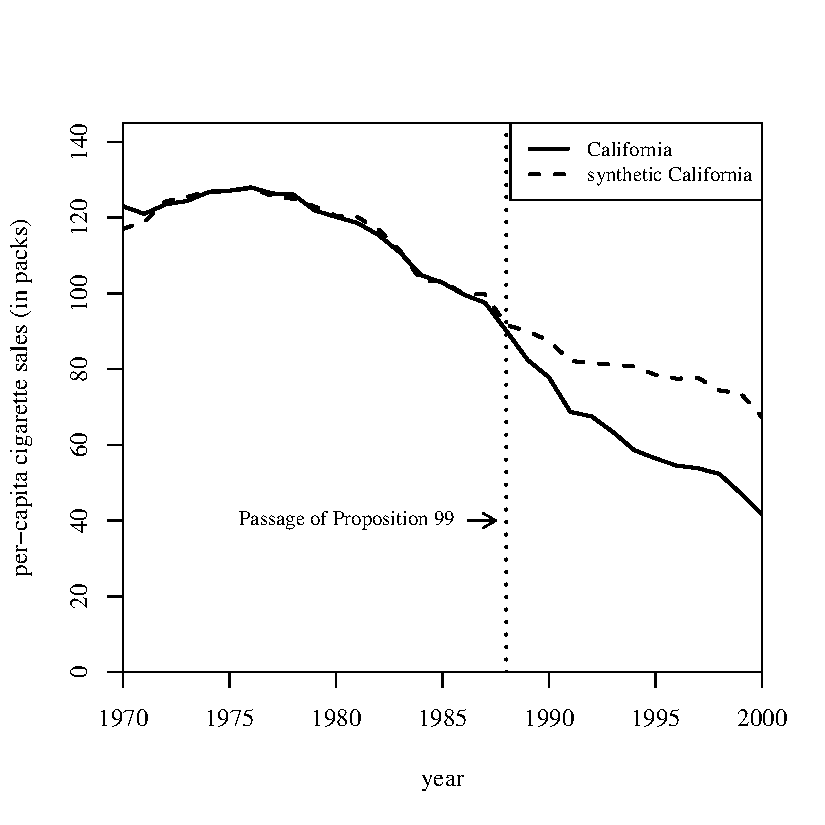
\includegraphics[width=\linewidth,height=1.5in,keepaspectratio,trim=2em 3em 2em 3em,clip]{ca2.pdf}}
  {Public policy}{California tobacco control}
\column{.32\textwidth}
\apppanel{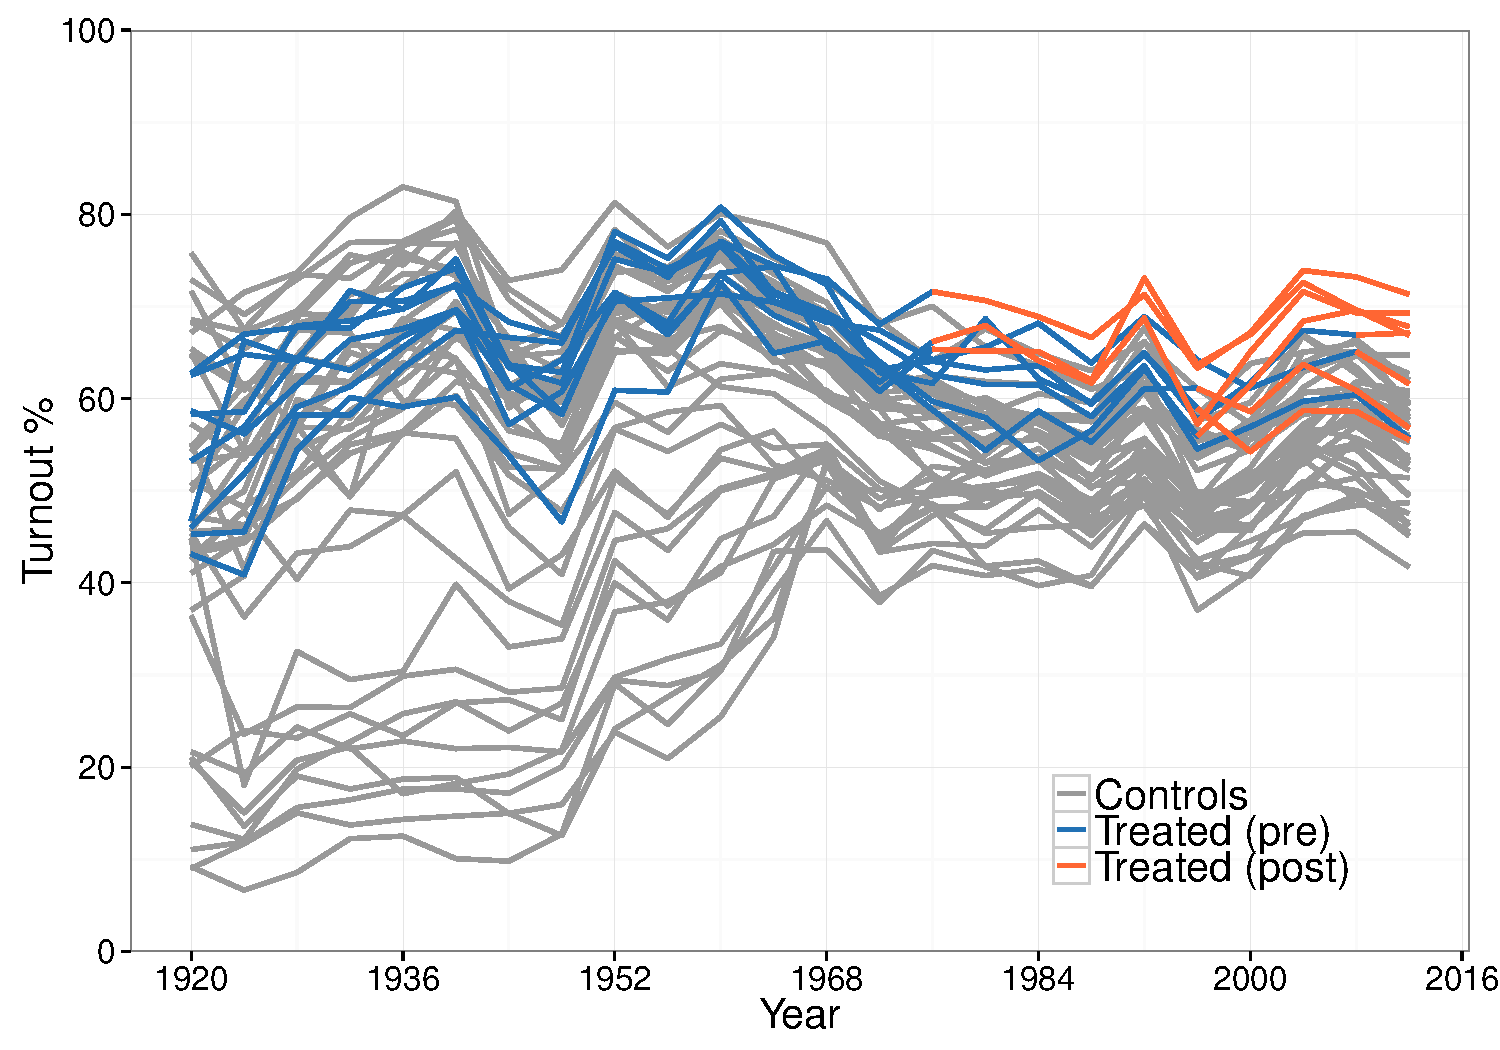
\includegraphics[width=\linewidth,height=1.5in,keepaspectratio]{edr_raw3.pdf}}
  {Political economy}{Election-day registration}
\column{.32\textwidth}
\apppanel{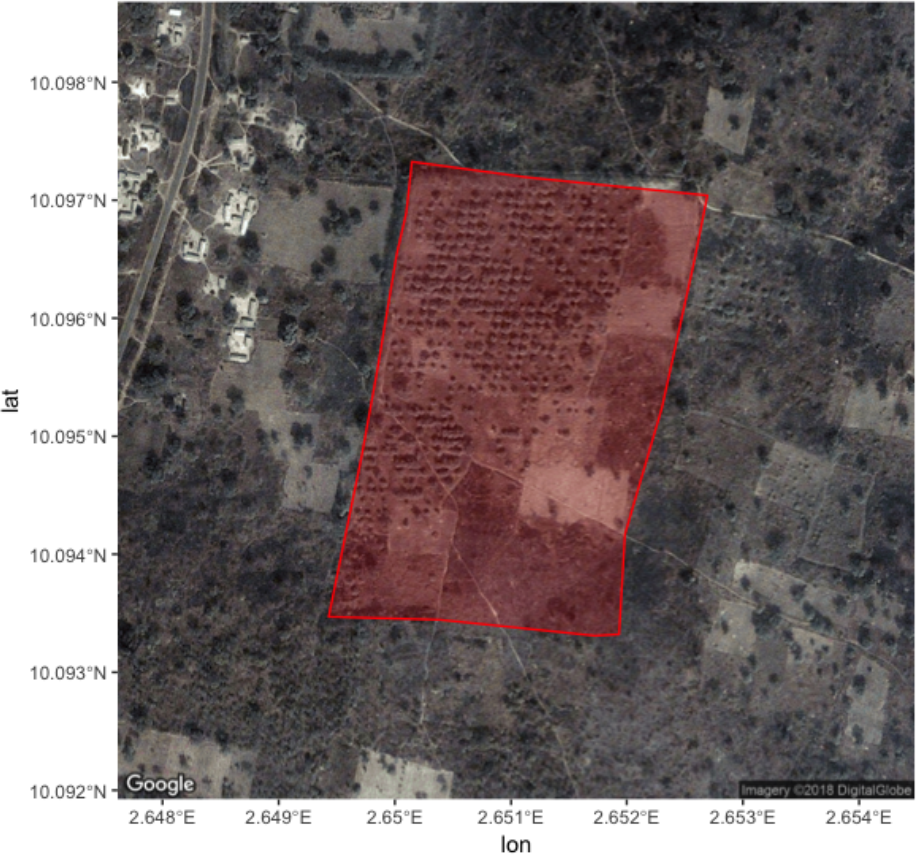
\includegraphics[width=\linewidth,height=1.5in,keepaspectratio]{benin_data2.png}}
  {Development}{Land titling in Benin}
\end{columns}
\slidesource{\textcite{abadie2010synthetic}; \textcite{xu2017generalized}; \textcite{sanford2019geospatial}.}
\end{frame}

\begin{frame}
\frametitle{The Literature in One Map}
\begin{center}
\begin{tabular}{p{.22\textwidth}p{.30\textwidth}p{.38\textwidth}}
\textbf{Family} & \textbf{What changes} & \textbf{Representative work} \\ \hline
Classic SCM & Convex donor weights & Abadie, Diamond, Hainmueller \\
Outcome models & Learn low rank structure & Xu; Athey et al. \\
Augmentation & Correct imperfect pre-fit & Ben-Michael, Feller, Rothstein \\
Synthetic DID & Weight units and time & Arkhangelsky et al. \\
\end{tabular}
\end{center}
\bigskip
\begin{block}{Common estimand}
Use outcomes from untreated units to estimate $Y_{1t}(0)$ after treatment.
\end{block}
\slidesource{\textcite{arkhangelsky2024causal}, survey of causal models for longitudinal and panel data.}
\end{frame}

\section{The Synthetic Control Method (SCM)}

\if\handout0{
\begin{frame}
\frametitle{SCM: Basic Idea}
\begin{itemize}
 \item<1-> $J+1$ units in periods $1, 2, \ldots, T$; one treated ``1'', $J$ controls
 \item<2-> Region ``1'' is exposed to the intervention after period $T_{0}$
 \item<5-> We aim to estimate the effect of the intervention on Region ``1''
\end{itemize}
\begin{center}
% yscale squeezes the coordinates without shrinking any node text; at full size
% this figure plus the three bullets overruns the 16:9 text height.
\begin{tikzpicture}[font=\small, yscale=0.74,
  donor/.style={fill=SlideBlue!16, draw=SlideBlue!55, thick, rounded corners=1.5pt},
  synth/.style={fill=SlideBlue, draw=SlideBlue, rounded corners=1.5pt},
  obs/.style={fill=SlideRed, draw=SlideRed, rounded corners=1.5pt}]
  % axes
  \draw[SlideInk!55, -{Latex[length=1.8mm]}] (0,0) -- (0,4.5);
  \draw[SlideInk!55, -{Latex[length=1.8mm]}] (0,0) -- (8.7,0);
  \node[left, text=SlideInk!75, font=\footnotesize] at (-0.12,3.68) {1};
  \node[left, text=SlideInk!75, font=\footnotesize] at (-0.12,1.52) {$J$};
  \node[below, text=SlideInk!75, font=\footnotesize] at (0.62,-0.08) {1};
  \node[below, text=SlideInk!75, font=\footnotesize] at (4.95,-0.08) {$T_0$};
  \node[below, text=SlideInk!75, font=\footnotesize] at (7.90,-0.08) {$T$};
  \node[rotate=90, text=SlideInk!55, font=\tiny] at (-0.62,2.5) {Units};
  \node[text=SlideInk!55, font=\tiny] at (4.3,-0.55) {Time};
  \draw[SlideInk!40, dashed, thick] (4.95,0) -- (4.95,4.2);
  % 3: the treated unit, observed before treatment
  \onslide<3->{\fill[obs] (0.60,3.50) rectangle (4.70,3.86);}
  % 4-5: the donor pool
  \onslide<4->{\fill[donor] (0.60,0.35) rectangle (4.70,2.72);}
  \onslide<5->{\fill[donor] (5.20,0.35) rectangle (7.90,2.72);}
  % 6-7: the cell we never observe
  \only<6-7>{\node[text=SlideRed, font=\large\bfseries] at (6.55,3.68) {?};}
  % 7: donor weights
  \onslide<7->{%
    \draw[SlideInk!70, thick, decorate,
          decoration={brace, amplitude=4pt, mirror}] (8.05,0.35) -- (8.05,2.72);
    \node[right, text=SlideInk, font=\footnotesize] at (8.22,1.52) {$w^{*}$};}
  % 8: the synthetic control
  \onslide<8->{%
    \fill[synth] (0.60,2.92) rectangle (4.70,3.28);
    \fill[synth] (5.20,2.92) rectangle (7.90,3.28);}
  % 9: match the pre-treatment path. The gap between the two bars is only ~2mm,
  % so the arrow needs a leader and a label placed in the clear space above.
  \onslide<9->{%
    \draw[{Latex[length=1.2mm]}-{Latex[length=1.2mm]}, SlideRed, thick]
      (2.65,3.50) -- (2.65,3.28);
    \draw[SlideInk!45, thin] (2.65,3.92) -- (2.65,4.12);
    \node[above, text=SlideInk!80, font=\tiny] at (2.65,4.12)
      {choose $w^{*}$ to close this gap before $T_0$};}
\end{tikzpicture}\\[0.3em]
\onslide<8->{\footnotesize\color{SlideInk!75}%
  \textcolor{SlideRed}{$\blacksquare$}~treated, observed \quad
  \textcolor{SlideBlue}{$\blacksquare$}~synthetic control \quad
  \textcolor{SlideBlue!45}{$\blacksquare$}~donor pool}
\end{center}
\end{frame}
}\else{
\begin{frame}
\frametitle{SCM: Basic Idea}
\begin{itemize}
 \item $J+1$ units in periods $1, 2, \ldots, T$; one treated ``1'', $J$ controls
 \item Region ``1'' is exposed to the intervention after period $T_{0}$
 \item We aim to estimate the effect of the intervention on Region ``1''
\end{itemize}
% Handout twin of the TikZ schematic above: same drawing with every step shown at
% once and no overlay specs. This branch previously still pulled the retired
% syn6.pdf, so the handout kept showing the old artwork while the projection
% deck showed the redraw. Keep the two in step when editing either.
\begin{center}
\begin{tikzpicture}[font=\small, yscale=0.74,
  donor/.style={fill=SlideBlue!16, draw=SlideBlue!55, thick, rounded corners=1.5pt},
  synth/.style={fill=SlideBlue, draw=SlideBlue, rounded corners=1.5pt},
  obs/.style={fill=SlideRed, draw=SlideRed, rounded corners=1.5pt}]
  \draw[SlideInk!55, -{Latex[length=1.8mm]}] (0,0) -- (0,4.5);
  \draw[SlideInk!55, -{Latex[length=1.8mm]}] (0,0) -- (8.7,0);
  \node[left, text=SlideInk!75, font=\footnotesize] at (-0.12,3.68) {1};
  \node[left, text=SlideInk!75, font=\footnotesize] at (-0.12,1.52) {$J$};
  \node[below, text=SlideInk!75, font=\footnotesize] at (0.62,-0.08) {1};
  \node[below, text=SlideInk!75, font=\footnotesize] at (4.95,-0.08) {$T_0$};
  \node[below, text=SlideInk!75, font=\footnotesize] at (7.90,-0.08) {$T$};
  \node[rotate=90, text=SlideInk!55, font=\tiny] at (-0.62,2.5) {Units};
  \node[text=SlideInk!55, font=\tiny] at (4.3,-0.55) {Time};
  \draw[SlideInk!40, dashed, thick] (4.95,0) -- (4.95,4.2);
  \fill[obs] (0.60,3.50) rectangle (4.70,3.86);
  \fill[donor] (0.60,0.35) rectangle (4.70,2.72);
  \fill[donor] (5.20,0.35) rectangle (7.90,2.72);
  \draw[SlideInk!70, thick, decorate,
        decoration={brace, amplitude=4pt, mirror}] (8.05,0.35) -- (8.05,2.72);
  \node[right, text=SlideInk, font=\footnotesize] at (8.22,1.52) {$w^{*}$};
  \fill[synth] (0.60,2.92) rectangle (4.70,3.28);
  \fill[synth] (5.20,2.92) rectangle (7.90,3.28);
  \draw[{Latex[length=1.2mm]}-{Latex[length=1.2mm]}, SlideRed, thick]
    (2.65,3.50) -- (2.65,3.28);
  \draw[SlideInk!45, thin] (2.65,3.92) -- (2.65,4.12);
  \node[above, text=SlideInk!80, font=\tiny] at (2.65,4.12)
    {choose $w^{*}$ to close this gap before $T_0$};
\end{tikzpicture}\\[0.3em]
{\footnotesize\color{SlideInk!75}%
  \textcolor{SlideRed}{$\blacksquare$}~treated, observed \quad
  \textcolor{SlideBlue}{$\blacksquare$}~synthetic control \quad
  \textcolor{SlideBlue!45}{$\blacksquare$}~donor pool}
\end{center}
\end{frame}
}
\fi


\begin{frame}
\frametitle{SCM: Insights}
\begin{itemize}\itemsep1em
\item \blue{\textcite{athey2017state}}: ``[a]rguably the most important innovation in the policy evaluation literature in the last 15 years.''\pause
\item A combo of many innovations\pause\medskip
\begin{itemize}\itemsep0.5em
	\item Take advantage of pre-treatment outcomes\pause
	\item Use cross-sectional instead of temporal correlations in data\pause
	\item Construct a convex combination of donors to construct a counterfactual\pause
	\item Reserve some pre-treatment periods for testing
\end{itemize}
\end{itemize}
\end{frame}

\if\handout0{
\begin{frame}[c]
\only<1-4>{\frametitle{Intuition}}
\only<5>{\frametitle{Difference-in-Differences (DID)}}
\only<6>{\frametitle{DID vs.\ Synthetic Control}}
\vspace{1em}
\begin{center}
\only<1>{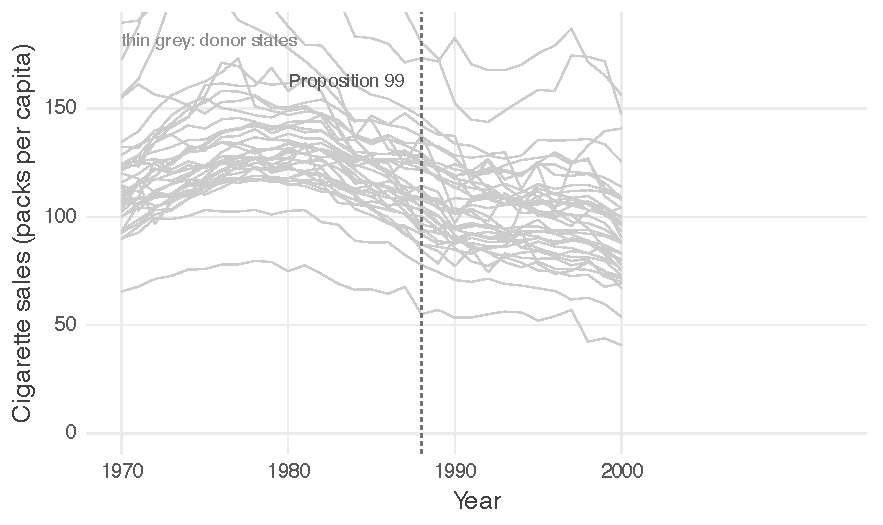
\includegraphics[width=0.70\textwidth]{scm_intuition1.pdf}}%
\only<2>{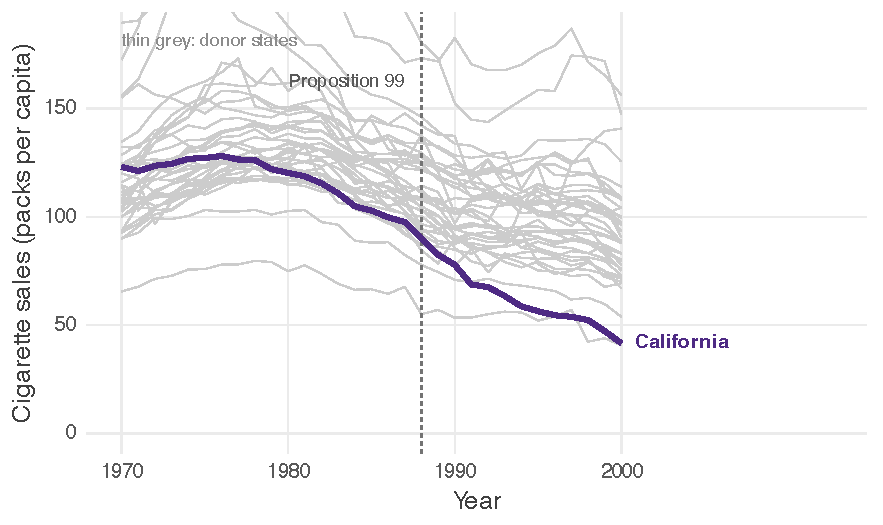
\includegraphics[width=0.70\textwidth]{scm_intuition2.pdf}}%
\only<3>{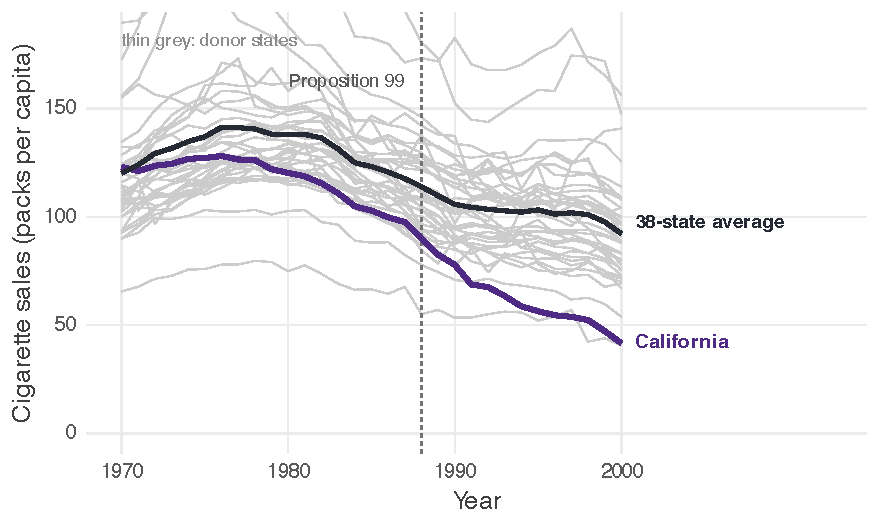
\includegraphics[width=0.70\textwidth]{scm_intuition3.pdf}}%
\only<4>{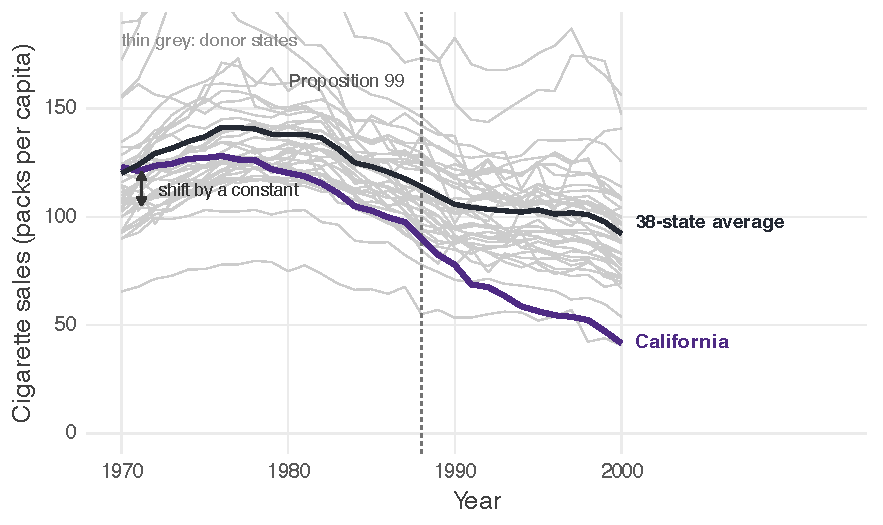
\includegraphics[width=0.70\textwidth]{scm_intuition4.pdf}}%
\only<5>{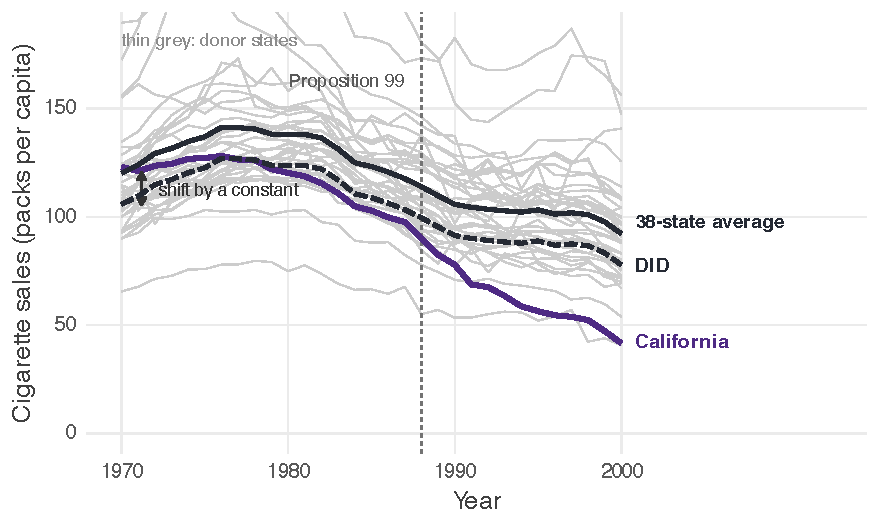
\includegraphics[width=0.70\textwidth]{scm_intuition5.pdf}}%
\only<6>{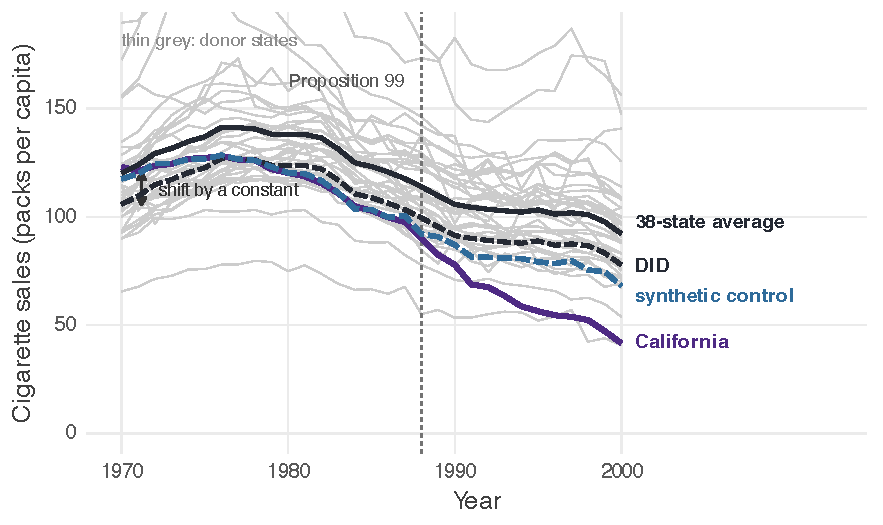
\includegraphics[width=0.70\textwidth]{scm_intuition6.pdf}}%
\end{center}
\end{frame}
}
\fi

\if\handout1{
\begin{frame}[c]
\frametitle{DID vs.\ Synthetic Control}
\vspace{1em}
\begin{center}
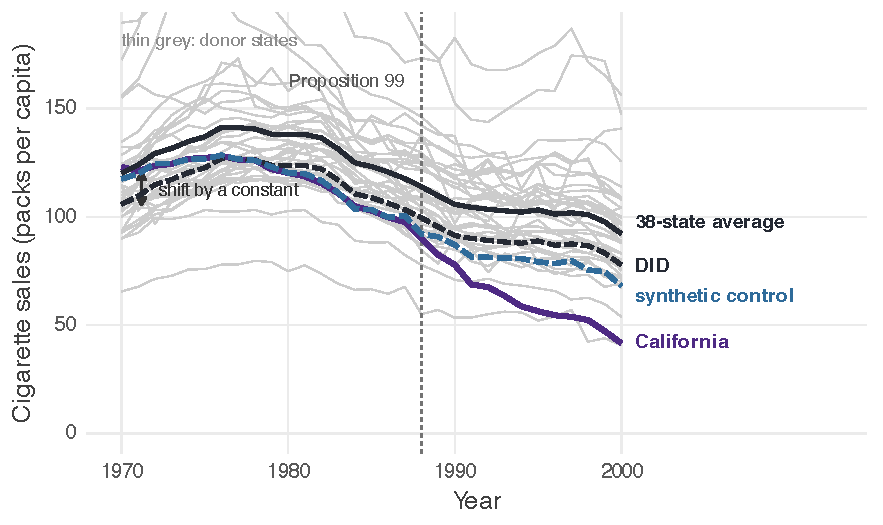
\includegraphics[width=0.70\textwidth]{scm_intuition6.pdf}
\end{center}
\end{frame}
}
\fi


\begin{frame}
\frametitle{Theoretical Justification}
\[
Y_{it} = \tau_{it}D_{it} + \theta_{t}'Z_{i} + \xi_{t} + \red{\lambda_{i}'f_{t}} + \varepsilon_{it}
\]\pause
\hspace{11.5em}\blue{or}
\[
  \hspace{-4em}\left\{
  \begin{array}{ll}
  Y_{it}(0) &=\ \theta_{t}'Z_{i} + \xi_{t} + \red{\lambda_{i}'f_{t}} + \varepsilon_{it}\\
  Y_{it}(1) &=\ Y_{it}(0) + \tau_{it} 
  \end{array}
  \right.
\]\pause
\begin{itemize}\itemsep0.5em
\item Suppose there are $R$ time-varying signals \red{$f_t$} out there\pause
\item Each unit (e.g. country, participant) picks up a fixed linear
  combination of these signals based on factor loadings \red{$\lambda_i$}\pause
\item Since these ``confounders'' are evidenced in the pre-treatment outcomes for both treated and controls, we can try to
  use this information to \blue{``balance on''} these confounders\pause
\item We will discuss the model-based approach later
\end{itemize}
\end{frame}

\begin{frame}
\frametitle{Theoretical Justification}
\[
\hspace{0em}\left\{
  \begin{array}{ll}
  Y_{it}(0) &=\ \theta_{t}'Z_{i} + \xi_{t} + \red{\lambda_{i}'f_{t}} + \varepsilon_{it}\\
  Y_{it}(1) &=\ Y_{it}(0) + \tau_{it} 
  \end{array}
  \right.
\]  
\begin{itemize}\itemsep0.5em
\item Let
$W=(w_2,\ldots,w_{J+1})'$ with $w_j\geq 0$ and
$w_2+\cdots +w_{J+1}=1$.
\item Let $\bar Y_i^{K_1},\ldots, \bar Y_i^{K_M}$ be \blue{$M>R$} linear
 functions of pre-intervention outcomes\pause
\item Suppose that we can choose $W^*$ such that:\medskip
\begin{center}
$Z_1 = \sum_{j=2}^{J+1} w^*_j Z_j,\quad
\bar Y_1^{k} = \sum_{j=2}^{J+1} w^*_j \bar
Y_j^{k},\ k \in \{K_{1},\ldots,K_M\}$
\end{center}\medskip
 \item When $T_{0}$ is large, an \red{approximately} unbiased estimator of $\tau_{1t}$ is:\medskip
\begin{center}
$\widehat \tau_{1t}=Y_{1t} - \sum_{j=2}^{J+1} w^*_j Y_{jt},\quad t\in\{T_0+1,\ldots ,T\}$
\end{center}
\end{itemize}
\end{frame}

\begin{frame}
\frametitle{Implementation}
\begin{itemize}\itemsep1em
\item Let $X_1=(Z_1, \bar Y^{K_1}_1, \ldots, \bar Y^{K_M}_1)'$ be a
$(k\times 1)$ vector of pre-intervention characteristics for the treated and $X_{0}$, a $(k\times J)$ matrix, for the controls.\pause
\item The vector $W^*$ is chosen to minimize $\|X_1-X_0 W\|$, subject to our weight
constraints.\pause\medskip
\begin{itemize}
\item We consider \blue{$\|X_1-X_0 W\|_V=\sqrt{(X_1-X_0 W)'V(X_1-X_0 W)}$},
     where $V$ is some $(k\times k)$ symmetric and positive
     semidefinite matrix.\medskip
\item Various ways to choose $V$ (subjective assessment of predictive
power of $X$, regression, minimize MSPE, cross-validation, etc.).
\end{itemize}
\end{itemize}
\end{frame}


\begin{frame}
\frametitle{Example: Proposition 99 on Cigarette Consumption}
\begin{itemize}
\item In 1988, California first passed comprehensive tobacco control legislation (cigarette tax, media campaign etc.)
\item Using 38 states that had never passed such programs as controls
\end{itemize}
  \begin{center}
  \hspace{-2em}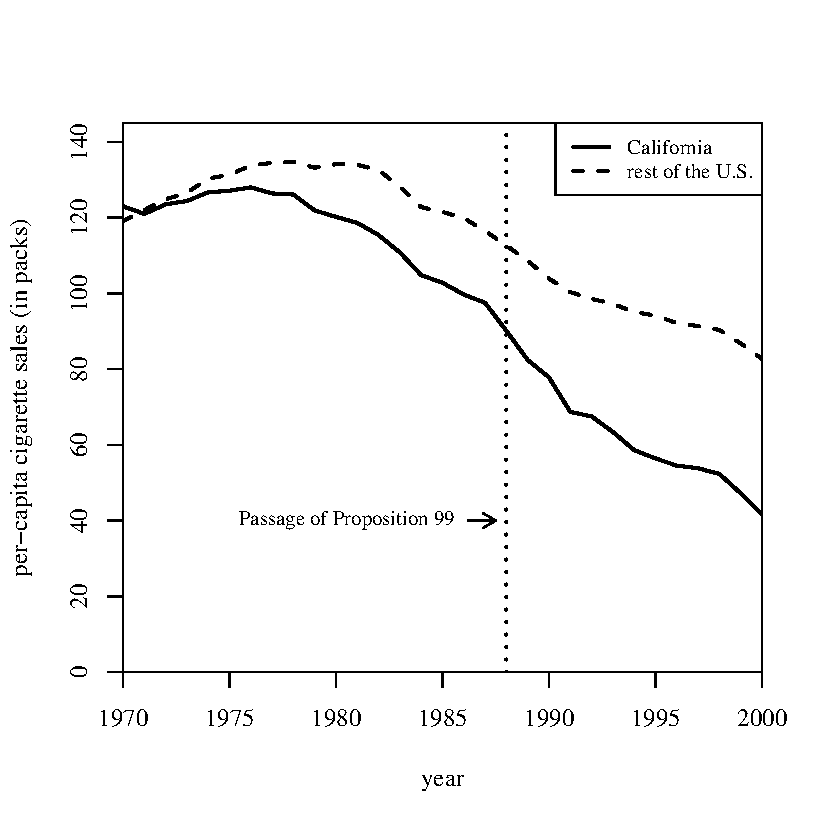
\includegraphics[height=2in,trim = 2em 3em 2em 3em, clip]{ca1.pdf}\\
  Cigarette Consumption: CA and the Rest of the U.S.
  \end{center}
\end{frame}

\begin{frame}
\frametitle{Example: Proposition 99 on Cigarette Consumption}
\begin{itemize}
\item In 1988, California first passed comprehensive tobacco control legislation (cigarette tax, media campaign etc.)
\item Using 38 states that had never passed such programs as controls
\end{itemize}
  \begin{center}
  \hspace{-2em}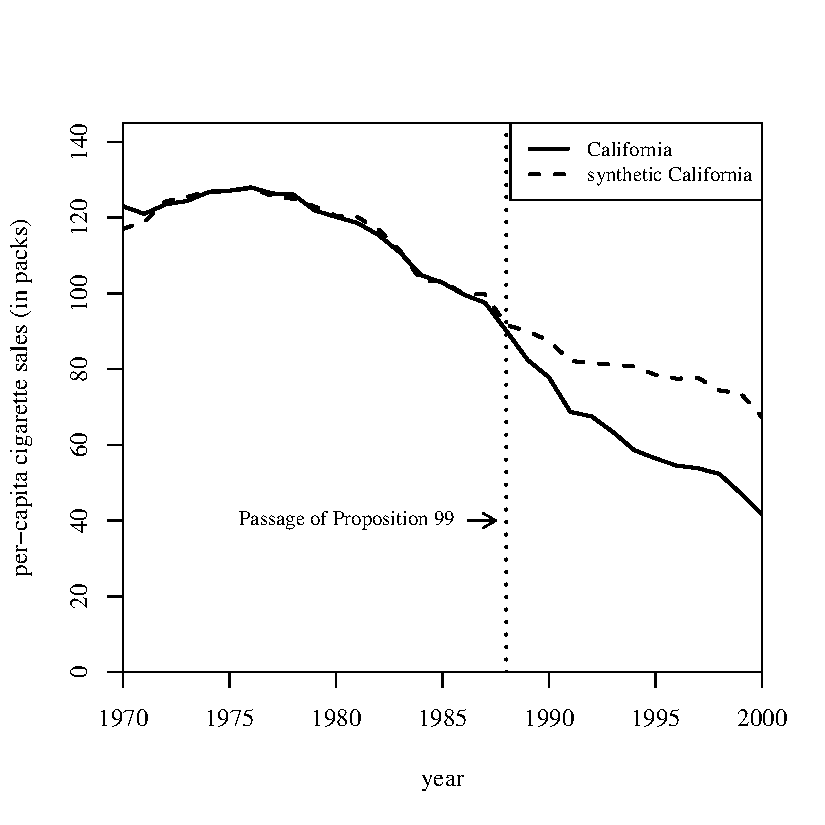
\includegraphics[height=2in,trim = 2em 3em 2em 3em, clip]{ca2.pdf}\\
  Cigarette Consumption: CA and Synthetic CA
  \end{center}
\end{frame}


\begin{frame}
\frametitle{Proposition 99: Gap, Placebos, and Inference}
\vspace{0.3em}
\begin{columns}[T,onlytextwidth]
\column{.32\textwidth}
\apppanel{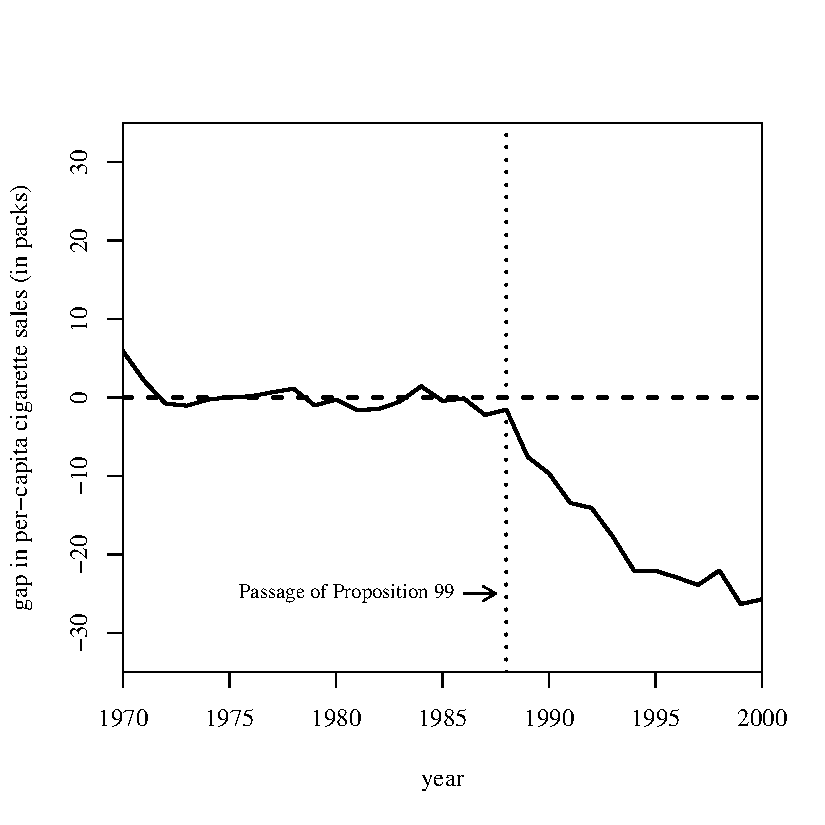
\includegraphics[width=\linewidth,height=1.5in,keepaspectratio]{ca3.pdf}}
  {1. The gap}{California minus synthetic California}
\column{.32\textwidth}
\apppanel{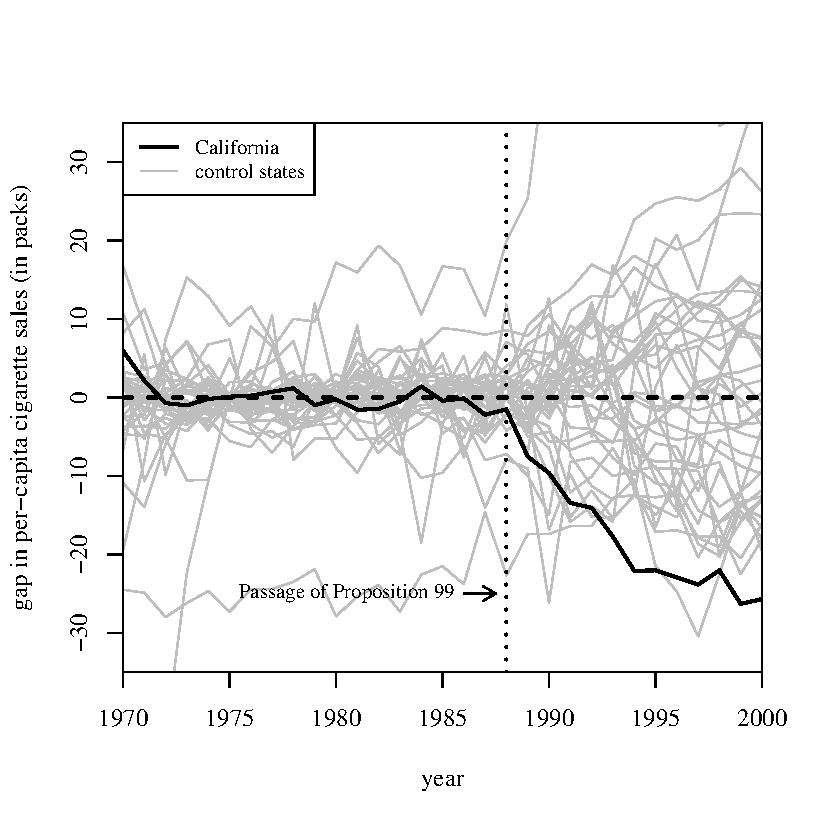
\includegraphics[width=\linewidth,height=1.5in,keepaspectratio]{ca4.pdf}}
  {2. Placebos}{Same gap computed for all 38 donor states}
\column{.32\textwidth}
\apppanel{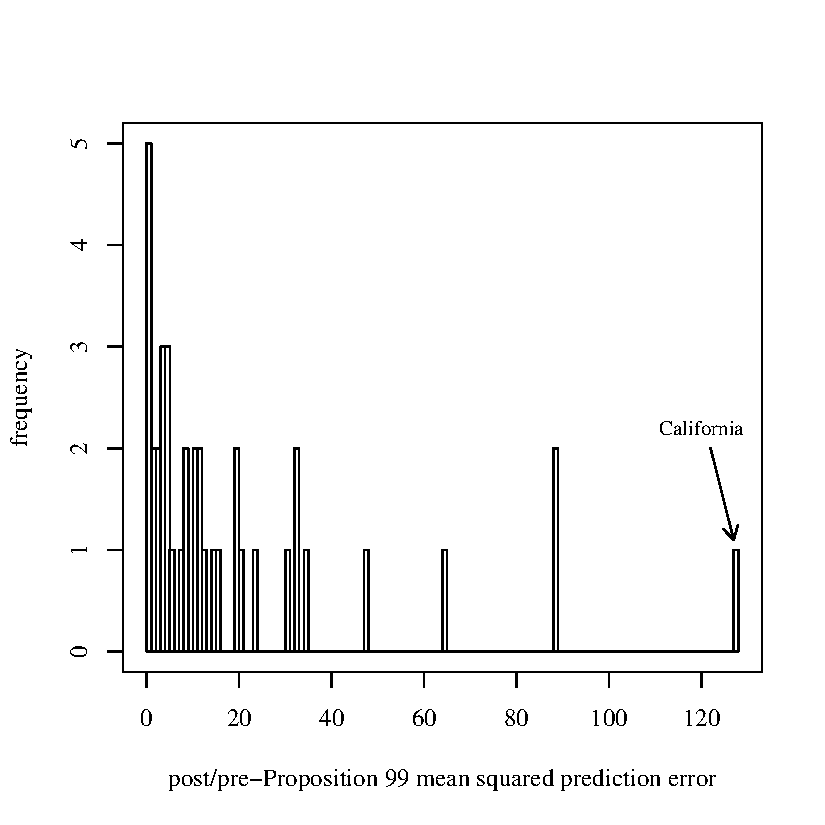
\includegraphics[width=\linewidth,height=1.5in,keepaspectratio]{ca8.pdf}}
  {3. Inference}{Ratio of post- to pre-treatment MSPE}
\end{columns}
\slidesource{\textcite{abadie2010synthetic}.}
\end{frame}


% Folded into the merged "Gap, Placebos, and Inference" slide above.

\begin{frame}
\frametitle{An Applied SCM Workflow}
\vspace{1.4em}
\begin{columns}[T]
\column{.23\textwidth}
\begin{block}{1. Fit}
Can donors reproduce the treated unit before treatment?
\end{block}
\column{.23\textwidth}
\begin{block}{2. Gap}
How does the treated-synthetic difference evolve after treatment?
\end{block}
\column{.23\textwidth}
\begin{block}{3. Placebo}
Would the method find similar gaps for untreated units?
\end{block}
\column{.23\textwidth}
\begin{block}{4. Stress test}
Do results survive donor and specification choices?
\end{block}
\end{columns}
\bigskip
For every application, show pre-treatment fit, the post-treatment gap, and the placebo distribution.
\slidesource{Cunningham, \emph{Causal Inference: The Mixtape}, synthetic control chapter.}
\end{frame}


\begin{frame}
 \frametitle{Limitations}
\begin{itemize}\itemsep1em
\item Algorithmic
\begin{itemize}
\item Deal with one treated unit at a time
\item Deal with one outcome at a time
\item Slow to implement and sometimes difficult to find a solution \pause
\item Allow too much user discretion, e.g. cherry-picking $\bar Y_{i}^{k}$ results in over-rejection (\blue{\citeshort{ferman2020cherry}})\pause
\end{itemize}
\item Inference
\begin{itemize}
\item Permutation inference and sensitivity analysis (e.g. {\blue{\cite{hahn2017synthetic}; \cite{firpo2018synthetic}; \citeshort{chernozhukov2021exact}}}) \pause
\item Inflated precision with nonstationary data (\blue{\citeshort{cattaneo2021prediction}})\pause
\end{itemize}
\item Identification
\begin{itemize}
\item My opinion: intrinsically, a method based on strict exogeneity (fixed timing)
\end{itemize}
\end{itemize}
\end{frame}


%%%%%%%%%%%%%%%%%%%%%%%%%%%%%%%%%%%%%%%%%%%%%%%%%%%%%%%%%%%%
%%%%%%%%%%%%%%%%%%%%%%%%%%%%%%%%%%%%%%%%%%%%%%%%%%%%%%%%%%%%%
%%%%%%%%%%%%%%%%%%%%%%%%%%%%%%%%%%%%%%%%%%%%%%%%%%%%%%%%%%%%%
%%%%%%%%%%%%%%%%%%%%%%%%%%%%%%%%%%%%%%%%%%%%%%%%%%%%%%%%%%%%%


\section{The Latent Factor Approach}

\begin{frame}
\frametitle{Link with Synthetic Control}
\begin{itemize}\itemsep0.5em 
\item Recall that ADH (\citeyear{abadie2010synthetic}) use a factor-augmented model to motivate the synthetic control method: 
\begin{center}
$Y_{it}(0) = \theta_{t}'Z_{i} + \xi_{t} + \red{\lambda_{i}'f_{t}} + \varepsilon_{it}$
\end{center}\pause
\item What if we actually estimate the model using observations under the control condition only? \pause 
\item \blue{\textcite{xu2017generalized}} imports the so-called interactive fixed effects (IFE) model into a DID setting
\begin{center}
$Y_{it}(0) = X_{it}'\beta + \alpha_{i} + \xi_{t} + \red{\lambda_{i}'f_{t}} + \varepsilon_{it}$
\end{center}\pause
\item \blue{\textcite{athey2021matrix}} extend it and introduce the matrix completion method
\item \blue{\textcite{liu2024practical}} put these methods in a general framework --- ``the counterfactual estimators'' \pause
\item \red{No negative weighting!}\pause
\item Limitations: needs large $T$ and $N$; model dependency
\end{itemize}
\end{frame}


\if\handout0{
\frame{
\frametitle{Basic Idea}
\begin{itemize}
  \item In a panel setting, treat the treated observations' $Y(0)$ as \red{missing data}
  \item<3-> Predict $Y(0)$ based on an \red{outcome model}
  \item[]<4-> (Use pre-treatment data for model selection)
  \item<5> Estimate ATT by averaging differences between $Y(1)$ and $\hat{Y}(0)$
\end{itemize}
\centering
\only<1,5>{
\includegraphics[width = 0.6\textwidth,height=1.55in,keepaspectratio]{sim_treat1.pdf}}%
\only<2-3>{
\includegraphics[width = 0.6\textwidth,height=1.55in,keepaspectratio]{sim_treat2.pdf}}%
\only<4>{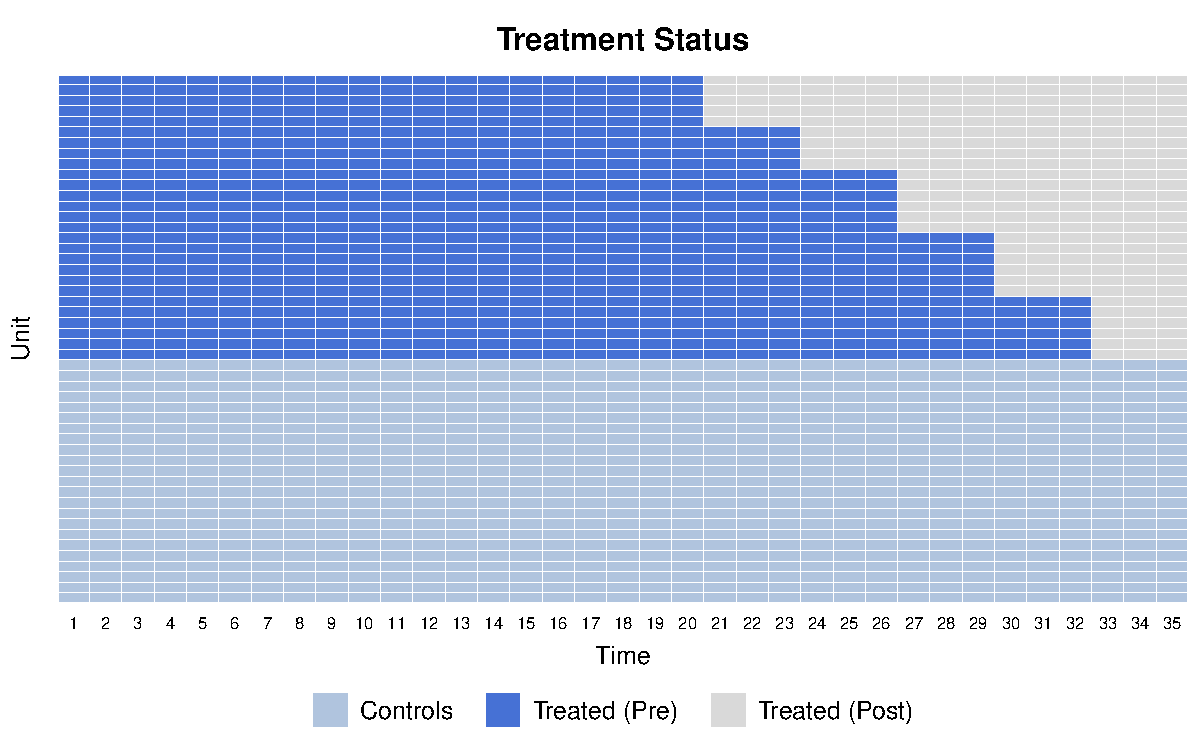
\includegraphics[width = 0.6\textwidth,height=1.55in,keepaspectratio]{sim_treat3.pdf}}%
}
}\else{
\frame{
\frametitle{Basic Idea}
\begin{itemize}
  \item In a panel setting, treat the treated observations' $Y(0)$ as \red{missing data}
  \item Predict $Y(0)$ based on an \red{outcome model}
  \item[] (Use pre-treatment data for model selection)
  \item Estimate ATT by averaging differences between $Y(1)$ and $\hat{Y}(0)$
\end{itemize}
\centering

\includegraphics[width = 0.6\textwidth,height=1.55in,keepaspectratio]{sim_treat1.pdf}%
}
}\fi


\frame{
\frametitle{Model-based Counterfactual Estimators}
A \underline{model-based} counterfactual estimator proceeds in the following steps:
\pause
\begin{itemize}\itemsep1em
\item Step 1. Train the model using observations under the control condition ($D_{it} = 0$). \pause
\item Step 2. Predict the counterfactual outcome $\hat{Y}_{it}(0)$ for each observation under the treatment condition ($D_{it} = 1$) and obtain an estimate of the individual treatment effect: $\hat{\tau}_{it} = Y_{it} - \hat{Y}_{it}(0).$\pause
\item Step 3. Generate estimates for the causal quantities of interest
 \[
 ATT = \E[\tau_{it}|D_{it}=1, \forall i\in\T, \forall t],\qquad\text{or}
 \]
 \[ATT_{s} = \E[\tau_{it}| D_{i,t-s}=0, \underbrace{D_{i,t-s+1} = D_{i,t-s+2} = \cdots =
  D_{it} = 1}_{s \text{ periods}}, \forall i\in\T].
 \]
\item[] {\footnotesize Indexing: $s$ counts periods under treatment, so $s = 1$ is the first treated period and $s = 0$ the last untreated one (the \texttt{fect} convention). Lecture 4's event-study specification indexed the same two periods as $s = 0$ and $s = -1$.}
\end{itemize}
}

\begin{frame}
\frametitle{Relative Time: Re-Indexing the Panel}
\begin{center}
\only<1| handout:0>{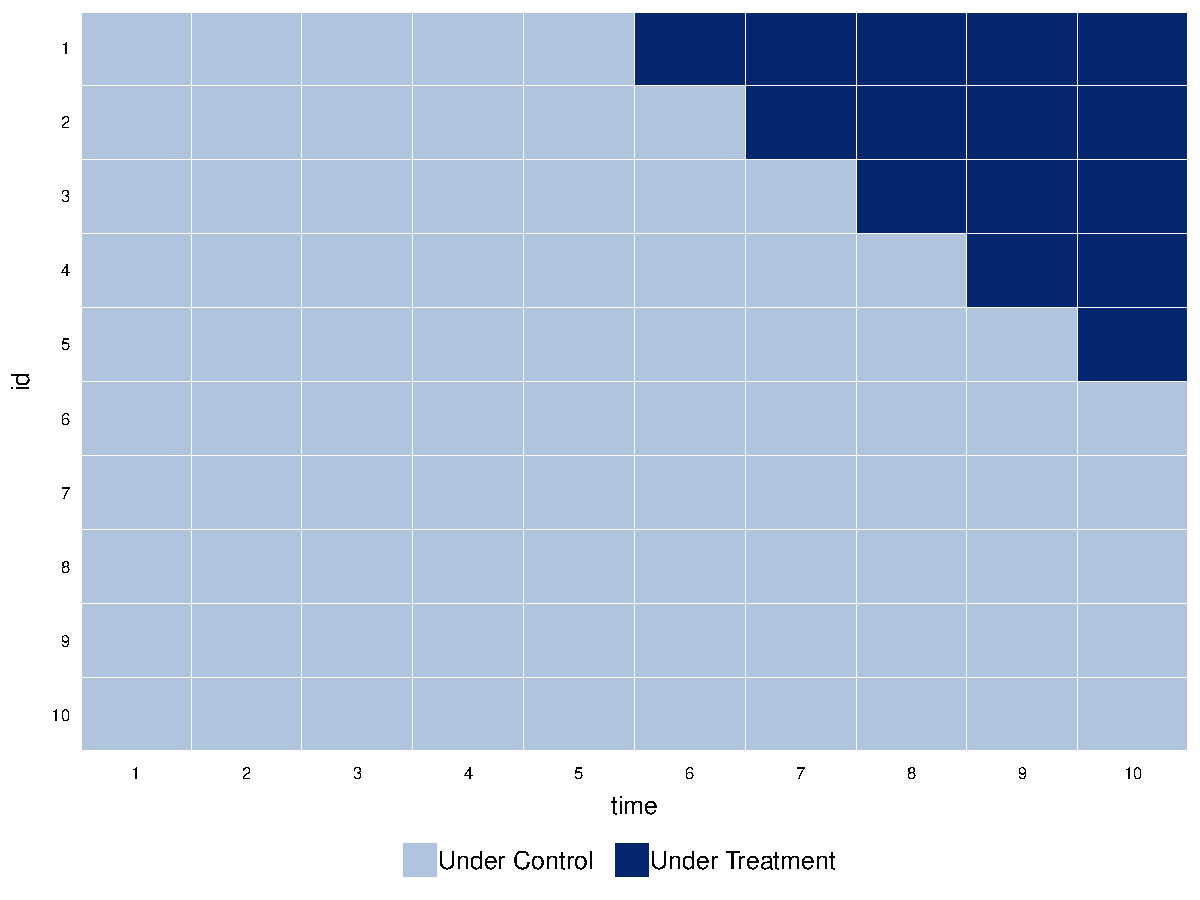
\includegraphics[height=0.66\textheight,keepaspectratio]{toy_default.pdf}}%
\only<2| handout:0>{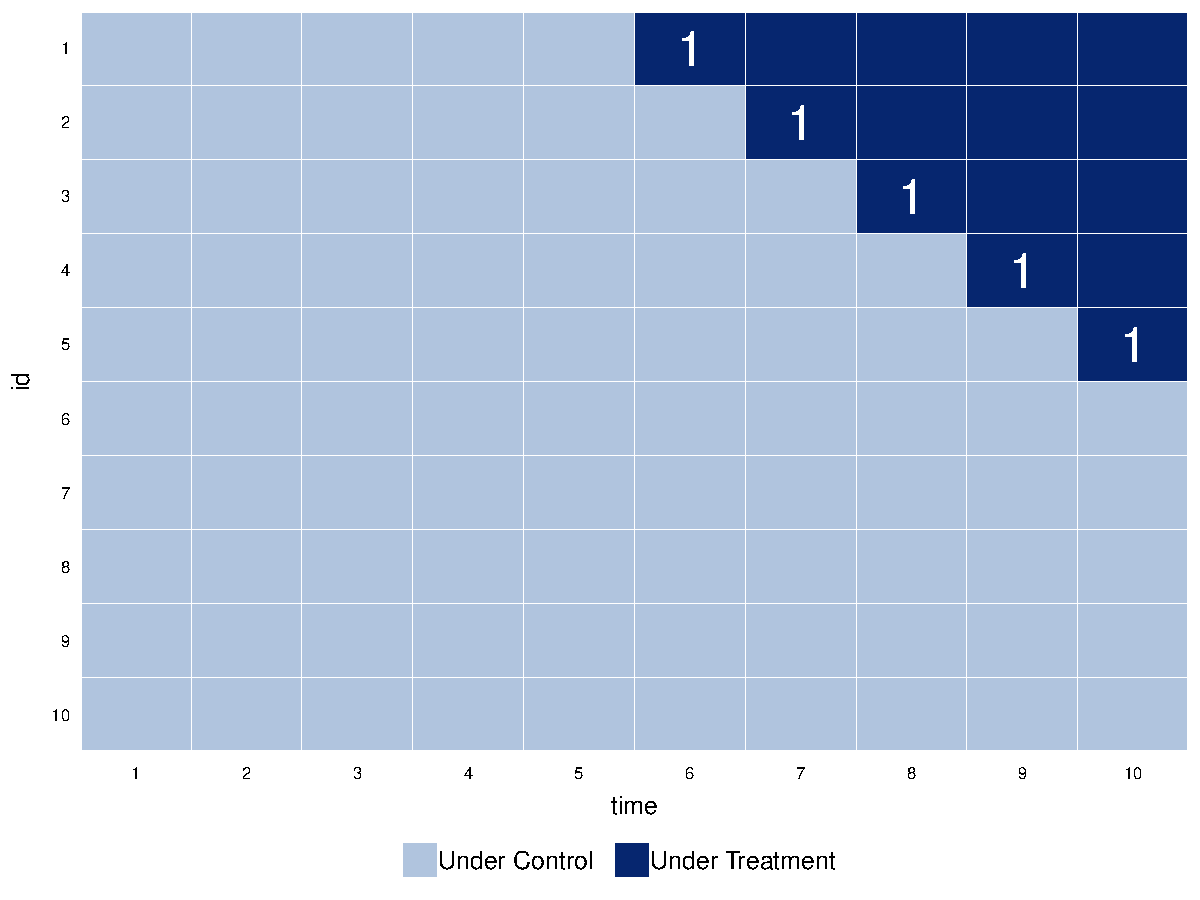
\includegraphics[height=0.66\textheight,keepaspectratio]{toy_1.pdf}}%
\only<3| handout:0>{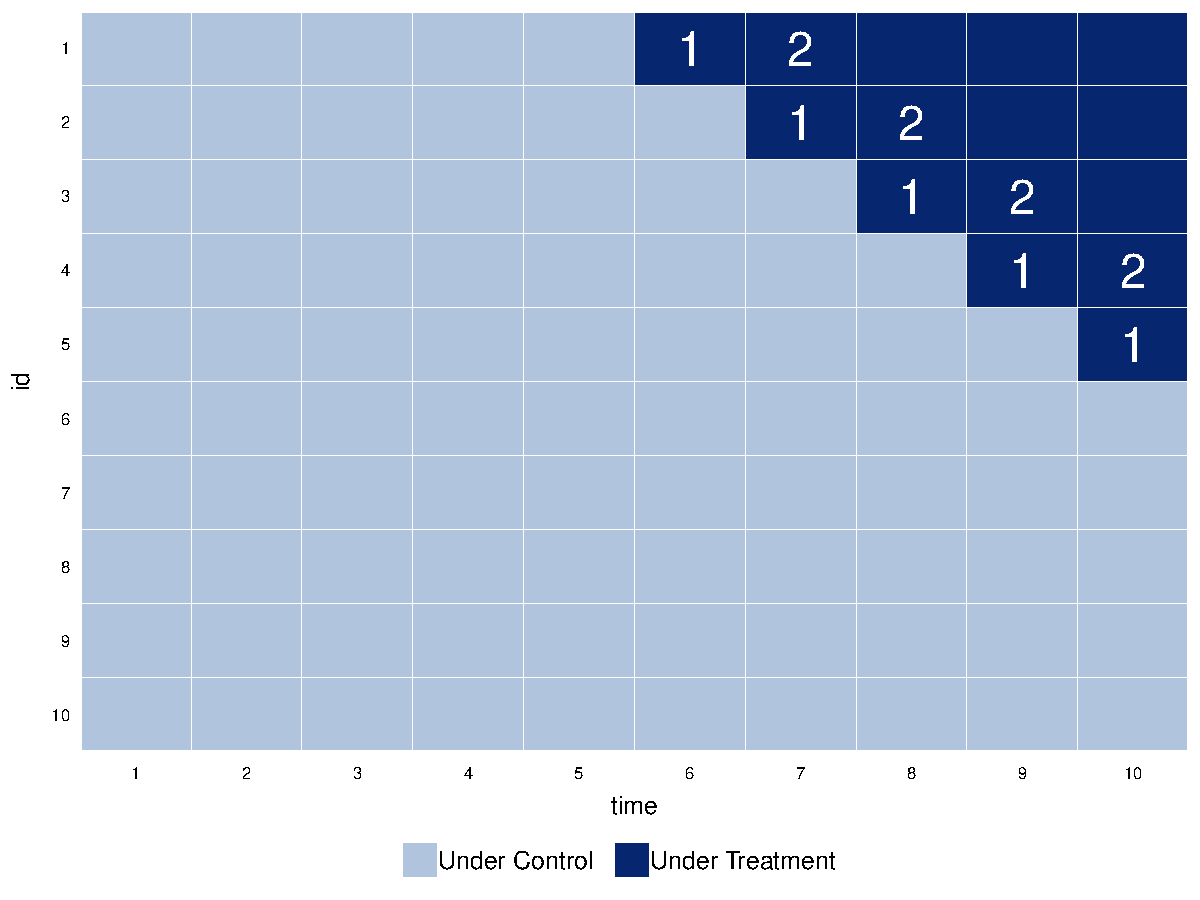
\includegraphics[height=0.66\textheight,keepaspectratio]{toy_2.pdf}}%
\only<4| handout:0>{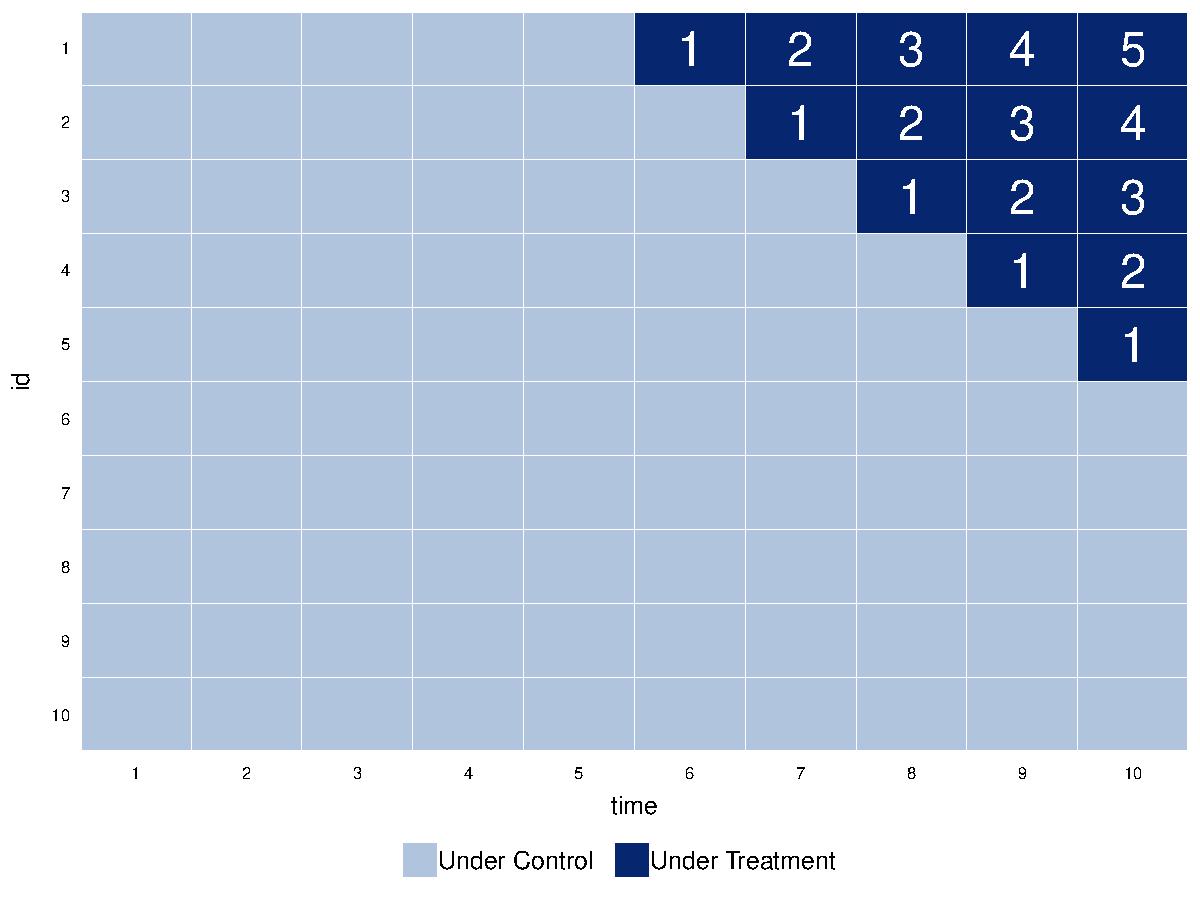
\includegraphics[height=0.66\textheight,keepaspectratio]{toy_3.pdf}}%
\only<5| handout:0>{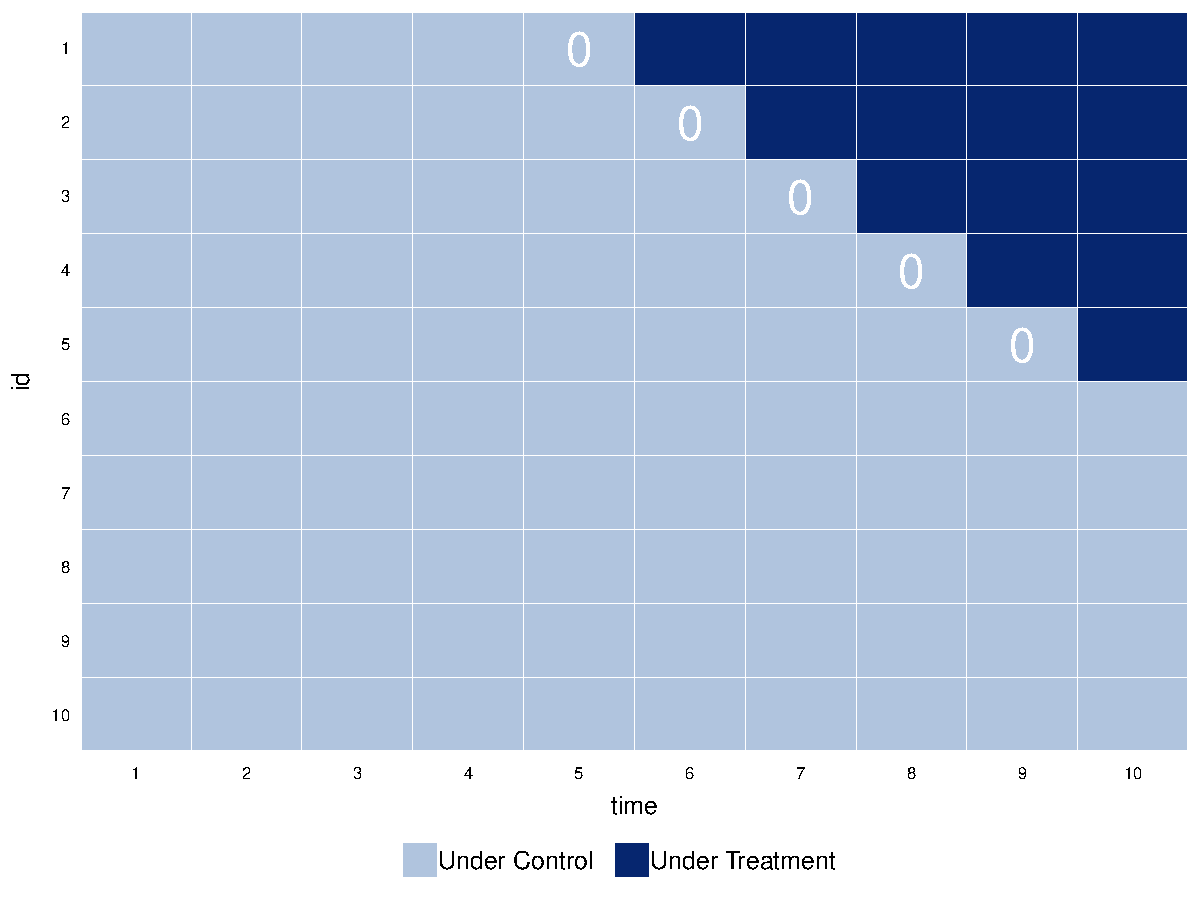
\includegraphics[height=0.66\textheight,keepaspectratio]{toy_4.pdf}}%
\only<6| handout:0>{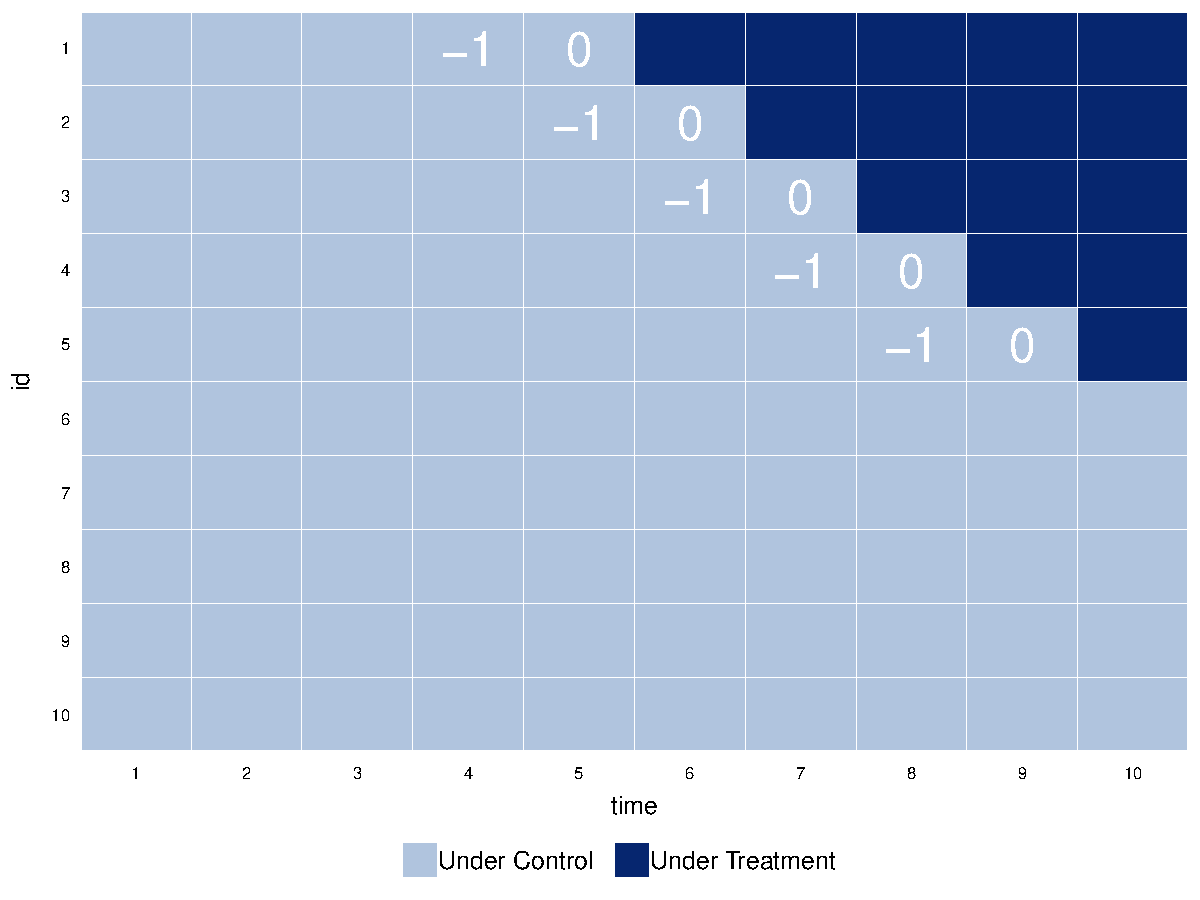
\includegraphics[height=0.66\textheight,keepaspectratio]{toy_5.pdf}}%
\only<7| handout:0>{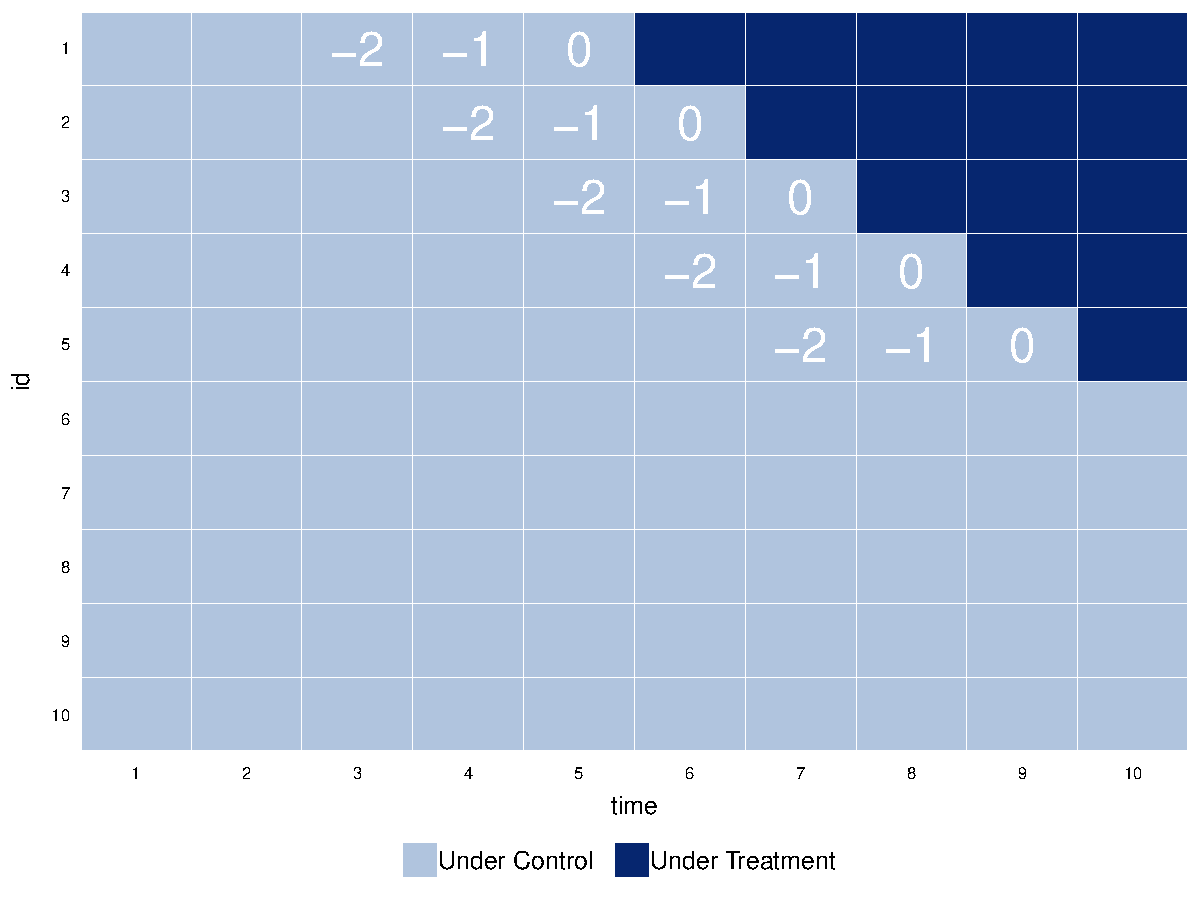
\includegraphics[height=0.66\textheight,keepaspectratio]{toy_6.pdf}}%
\only<8| handout:0>{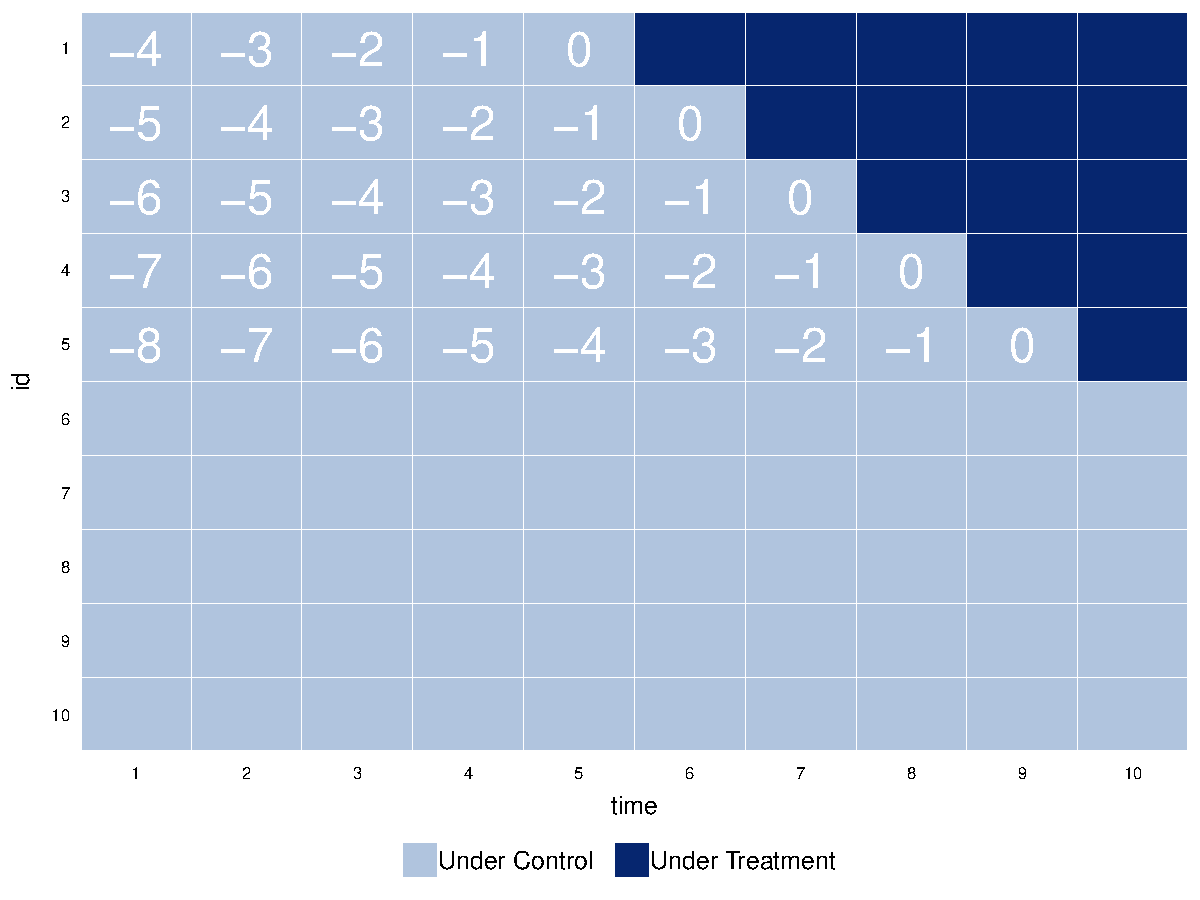
\includegraphics[height=0.66\textheight,keepaspectratio]{toy_7.pdf}}%
\only<9| handout:1>{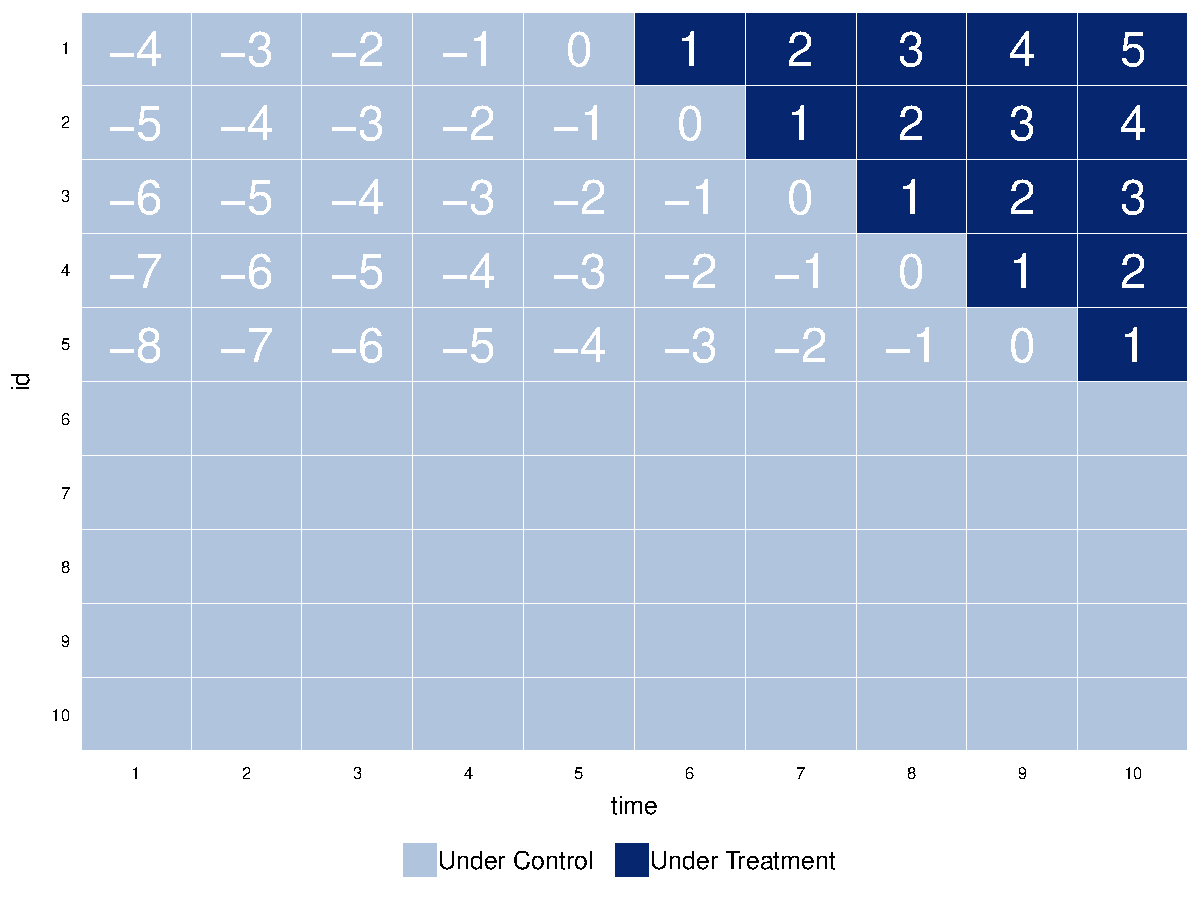
\includegraphics[height=0.66\textheight,keepaspectratio]{toy_8.pdf}}%
\end{center}
\begin{itemize}
\item<9-| handout:1> Each treated observation is re-indexed by its distance to the adoption date, with $s = 1$ the first treated period and $s = 0$ the last untreated one; $\widehat{ATT}_s$ averages within a diagonal
\end{itemize}
\end{frame}

\begin{frame}
\frametitle{Reading a Dynamic Treatment Effects Plot}
\begin{center}
\only<1| handout:0>{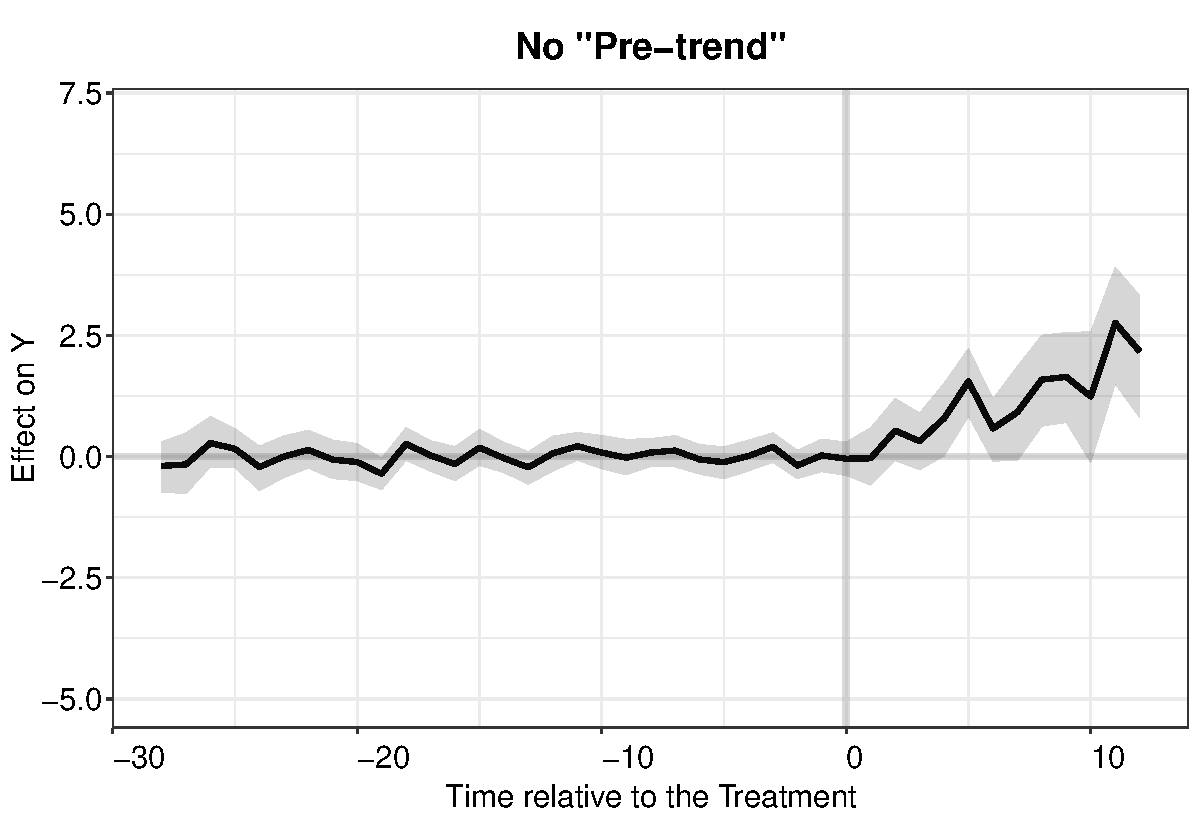
\includegraphics[height=0.62\textheight,keepaspectratio]{sim_dyn_1.pdf}}%
\only<2| handout:1>{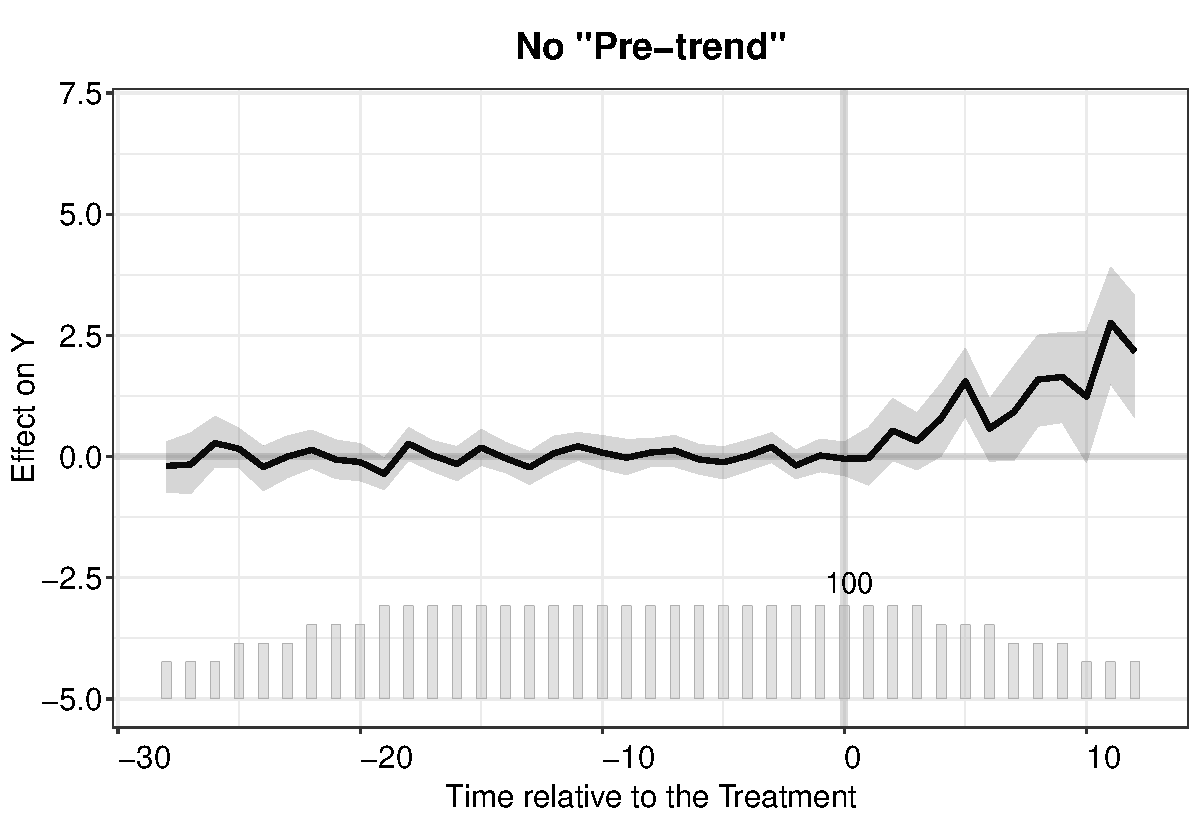
\includegraphics[height=0.62\textheight,keepaspectratio]{sim_dyn_2.pdf}}%
\end{center}
\begin{itemize}
\item<2-| handout:1> Pre-treatment averages are close to zero; post-treatment averages step up: no visible pre-trend
\item<2-| handout:1> The gray bars at the bottom show how many observations each average uses; distant leads and lags rest on few observations
\end{itemize}
\end{frame}

\begin{frame}
\frametitle{The Warning Sign: A Pre-Trend}
\begin{center}
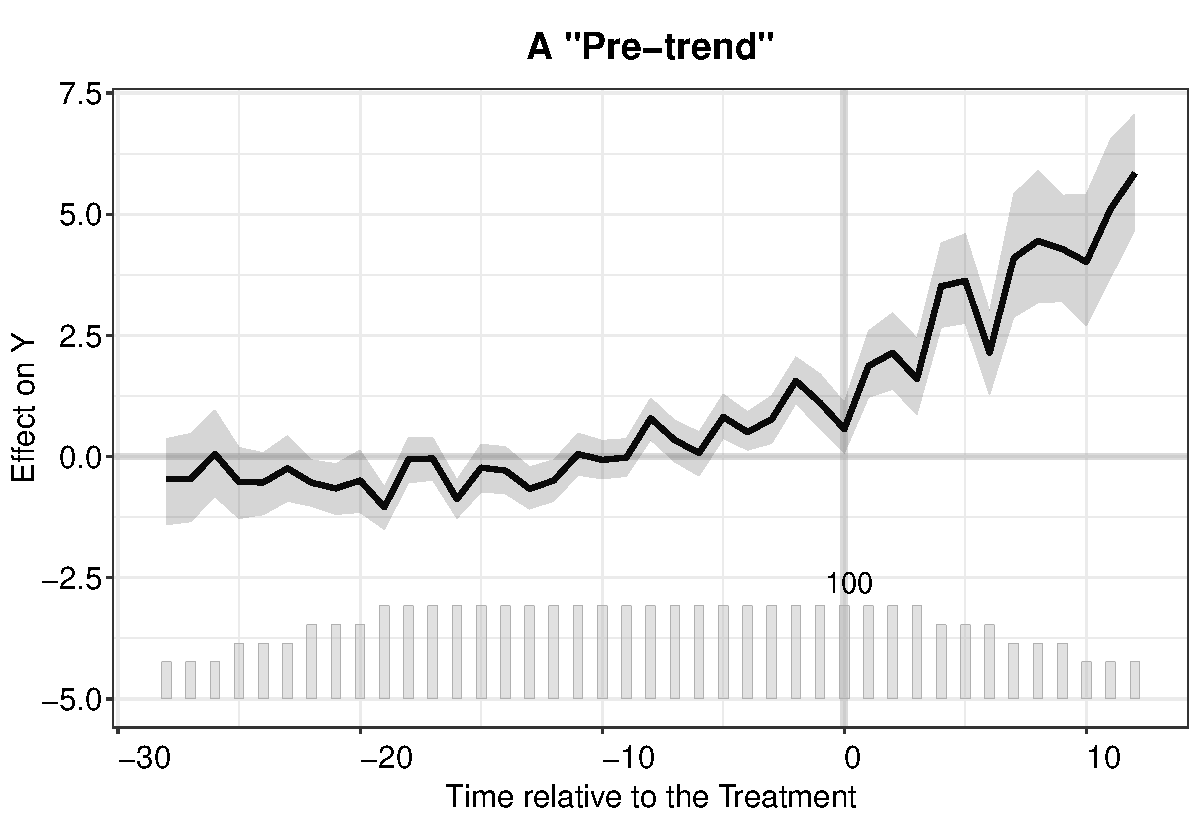
\includegraphics[height=0.62\textheight,keepaspectratio]{sim_dyn_3.pdf}
\end{center}
\begin{itemize}
\item<2-> Pre-treatment averages drift away from zero: the comparison units were already on a different path, and the post-treatment estimates inherit that drift
\end{itemize}
\end{frame}

\frame{
\frametitle{Review of Three Estimators}

We review three estimation strategies:
\begin{itemize}\itemsep0.5em
\item FEct:\\
 \begin{center}
 $\hat{Y}_{it}(0) = X_{it}\hat{\beta} + \hat{\alpha}_i + \hat{\xi}_t$
 \end{center}\pause
\item IFEct {\small \blue{\parencite{gobillon2016regional,xu2017generalized}}}:\\
 \begin{center}
 $\hat{Y}_{it}(0) = X_{it}\hat{\beta} + \hat{\lambda}_i^{\prime} \hat{f}_t$
 \end{center}
\pause
\item Matrix Completion (MC) {\small \blue{\parencite{athey2021matrix}}}:\\
 \begin{center}$\hat{Y}_{it}(0) = X_{it}\hat{\beta} + \hat{L}_{it},$
 \end{center}
 where matrix $\{L_{it}\}_{N \times T}$
  is a lower-rank matrix approximation of $\{Y(0)\}_{N \times T}$ with missing values 
\end{itemize}
\pause
\vspace{4pt}

{\bf Remarks}:
\begin{itemize}
\item DID is a special case of FEct\pause
\item Both IFEct and MC are estimated via iterative algorithms\pause
\item Cross-validation to choose the tuning parameter
\end{itemize}
}

\if\handout0{
\begin{frame}
 \frametitle{IFEct}
\vspace{1em}
\textcite{xu2017generalized} proposes a three-step approach based on a latent factor model:\vspace{-0.5em}
\only<1>{ 
\begin{eqnarray*}
\mbox{\blue{Control }}\quad Y_{it}(0) &=&  X_{it}'\beta + \alpha_{i}  + \xi_{t} + \lambda_{i}^{\prime} f_{t} + \varepsilon_{it} \phantom{\hspace{5.7em}}
\end{eqnarray*}\vspace{4.2em}
}%
\only<2,11->{ 
\begin{eqnarray*}
\mbox{\blue{Control }}\quad Y_{it}(0) &=& X_{it}'\beta + \alpha_{i}  + \xi_{t} + \lambda_{i}^{\prime} f_{t} + \varepsilon_{it} \\
\mbox{\blue{Treated}}\ \quad Y_{it}(0) &=& X_{it}'\beta + \alpha_{i}  + \xi_{t} + \lambda_{i}^{\prime} f_{t} + \varepsilon_{it}  \phantom{\hspace{3.2em}}\mbox{\blue{(pre)}} \\
Y_{it}(1) &=& X_{it}'\beta + \alpha_{i}  + \xi_{t} + \lambda_{i}^{\prime} f_{t} + \varepsilon_{it} + \tau_{it} \quad\mbox{\blue{(post)}}
\end{eqnarray*}\vspace{1em}
}%
\only<3-5>{ 
\begin{eqnarray*}
\mbox{\blue{Control }}\quad Y_{it}(0) &=& \lambda_{i}^{\prime} f_{t} + \varepsilon_{it} \\
\mbox{\blue{Treated }}\quad Y_{it}(0) &=& \lambda_{i}^{\prime} f_{t} + \varepsilon_{it} \phantom{\hspace{3.2em}}\mbox{\blue{(pre)}}\\
                           Y_{it}(1) &=& \lambda_{i}^{\prime} f_{t} + \varepsilon_{it} + \tau_{it}\quad\mbox{\blue{(post)}} \phantom{\hspace{7.3em}}
\end{eqnarray*}\vspace{1em}
}%
\only<6-7>{ 
\begin{eqnarray*}
\mbox{\blue{Control }}\quad Y_{it}(0) &=& \red{\lambda_{i}^{\prime} f_{t}} + \varepsilon_{it} \\
\mbox{\blue{Treated }}\quad Y_{it}(0) &=& \lambda_{i}^{\prime} f_{t} + \varepsilon_{it} \phantom{\hspace{3.2em}}\mbox{\blue{(pre)}}\\
                           Y_{it}(1) &=& \lambda_{i}^{\prime} f_{t} + \varepsilon_{it} + \tau_{it} \quad\mbox{\blue{(post)}} \phantom{\hspace{7.3em}}
\end{eqnarray*}\vspace{1em}
}%
\only<8>{ 
\begin{eqnarray*}
\mbox{\blue{ Control }}\quad Y_{it}(0) &=& \red{\lambda_{i}^{\prime} f_{t}} + \varepsilon_{it} \\
\mbox{\blue{Treated }}\quad Y_{it}(0) &=& \lambda_{i}^{\prime} \red{f_{t}} + \varepsilon_{it} \phantom{\hspace{3.2em}}\mbox{\blue{(pre)}}\\
                           Y_{it}(1) &=& \lambda_{i}^{\prime} f_{t} + \varepsilon_{it} + \tau_{it} \quad\mbox{\blue{(post)}} \phantom{\hspace{7.3em}}
\end{eqnarray*}\vspace{1em}
}%
\only<9>{ 
\begin{eqnarray*}
\mbox{\blue{Control }}\quad Y_{it}(0) &=& \red{\lambda_{i}^{\prime} f_{t}} + \varepsilon_{it} \\
\mbox{\blue{Treated }}\quad Y_{it}(0) &=& \red{\lambda_{i}^{\prime} f_{t}} + \varepsilon_{it} \phantom{\hspace{3.2em}}\mbox{\blue{(pre)}}\\
                           Y_{it}(1) &=& \lambda_{i}^{\prime} f_{t} + \varepsilon_{it} + \tau_{it} \quad\mbox{\blue{(post)}} \phantom{\hspace{7.3em}}
\end{eqnarray*}\vspace{1em}
}%
\only<10>{ 
\begin{eqnarray*}
\mbox{\blue{Control }}\quad Y_{it}(0) &=& \red{\lambda_{i}^{\prime} f_{t}} + \varepsilon_{it} \\
\mbox{\blue{Treated }}\quad Y_{it}(0) &=& \red{\lambda_{i}^{\prime} f_{t}} + \varepsilon_{it} \phantom{\hspace{3.2em}}\mbox{\blue{(pre)}}\\
                           Y_{it}(1) &=& \lambda_{i}^{\prime} f_{t} + \varepsilon_{it} + \red{\tau_{it}} \quad\mbox{\blue{(post)}} \phantom{\hspace{7.3em}}
\end{eqnarray*}
}%
\vspace{-1em}
\begin{columns}[c]
% left column
\begin{column}{.45\textwidth}
\vspace{-2em}
\begin{enumerate}
\item<6-> Estimate using controls
\item<8-> Predict on treated $\widehat{Y}_{it}(0)$
\item<9-> Calculate the ATT
\item<10-> Expectation-Maximization\\{\footnotesize\blue{\parencite{gobillon2016regional}}}
\end{enumerate}
\end{column}
% right column
\begin{column}{.55\textwidth}
\vspace{-1em}
\only<4>{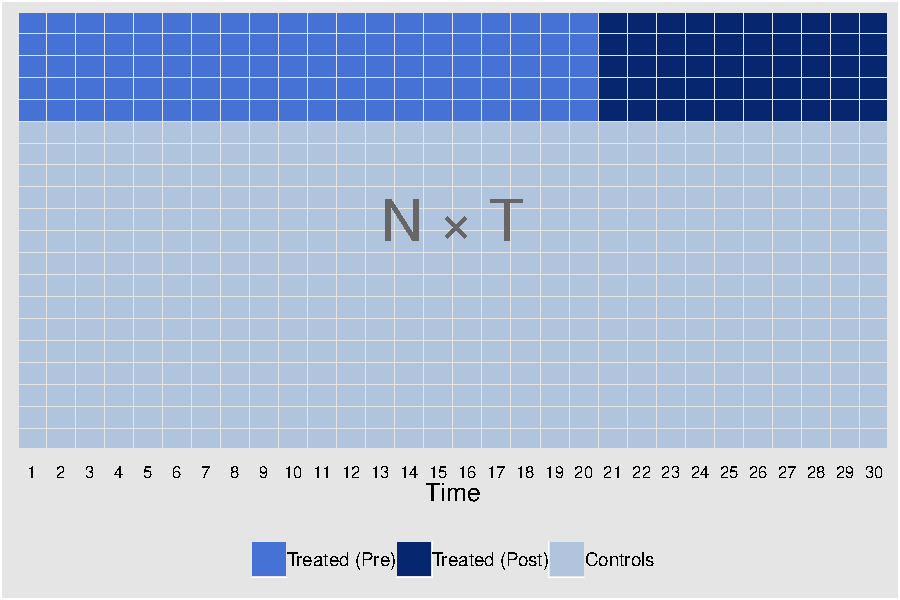
\includegraphics[width=\textwidth,height=1.75in,keepaspectratio]{sim_status1a.pdf}}%
\only<5>{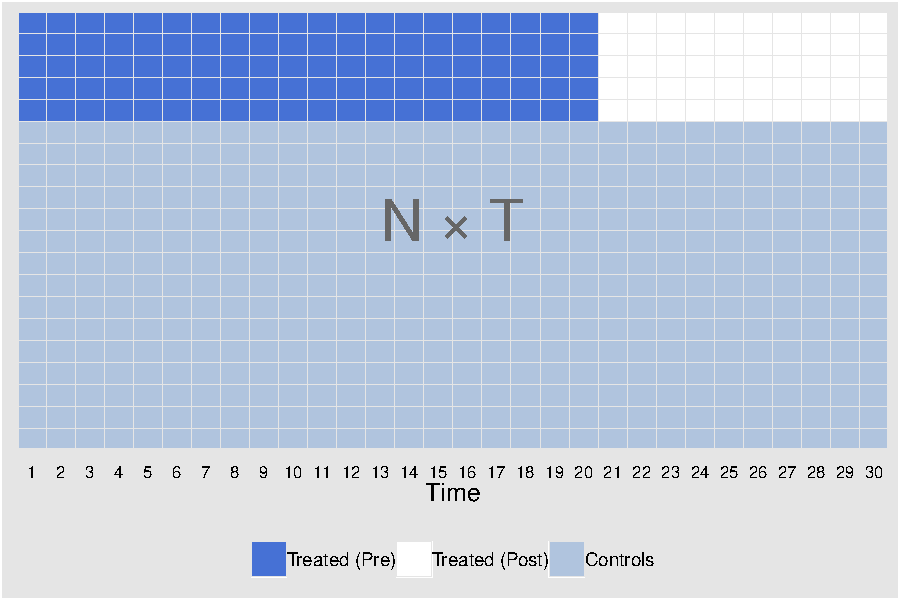
\includegraphics[width=\textwidth,height=1.75in,keepaspectratio]{sim_status2a.pdf}}%
\only<6>{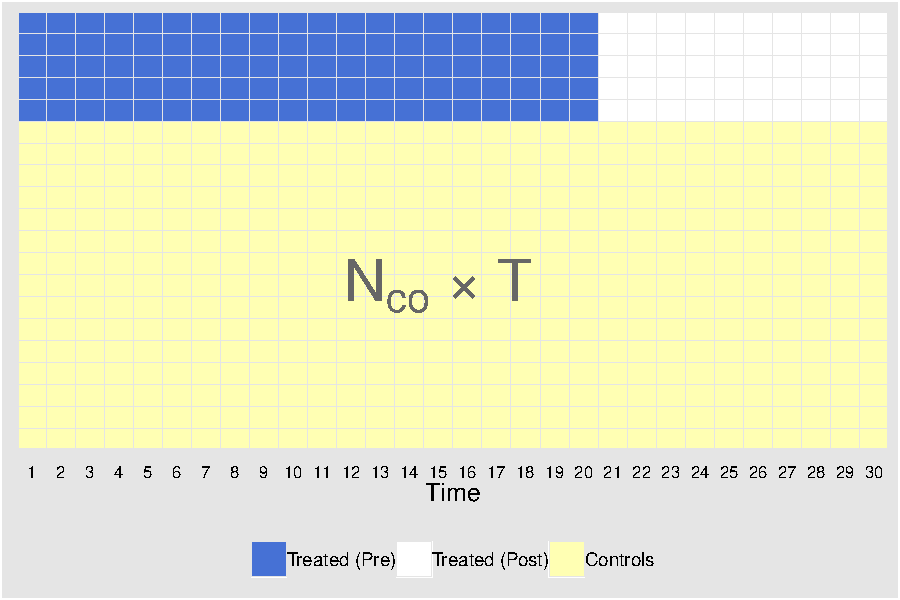
\includegraphics[width=\textwidth,height=1.75in,keepaspectratio]{sim_status3a.pdf}}%
\only<7>{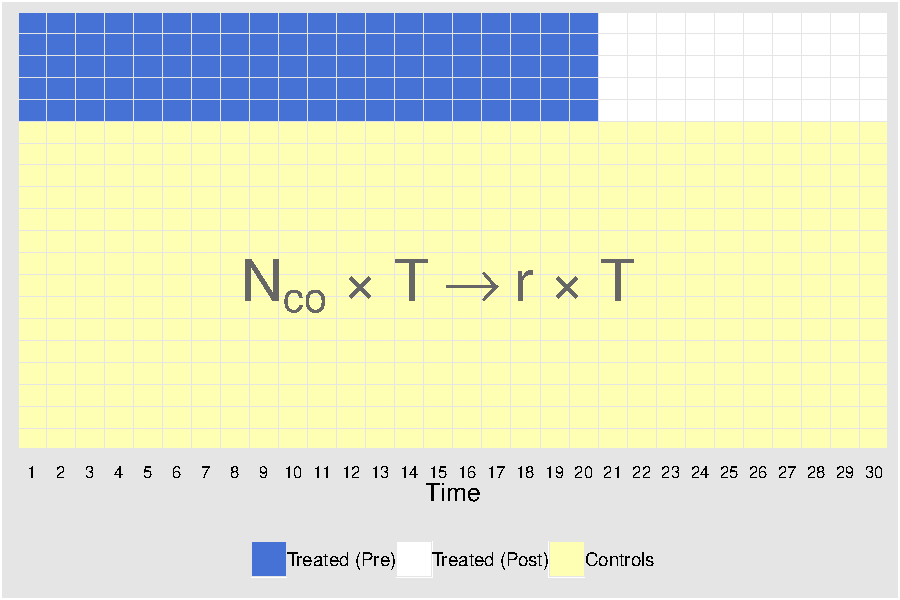
\includegraphics[width=\textwidth,height=1.75in,keepaspectratio]{sim_status3b.pdf}}%
\only<8>{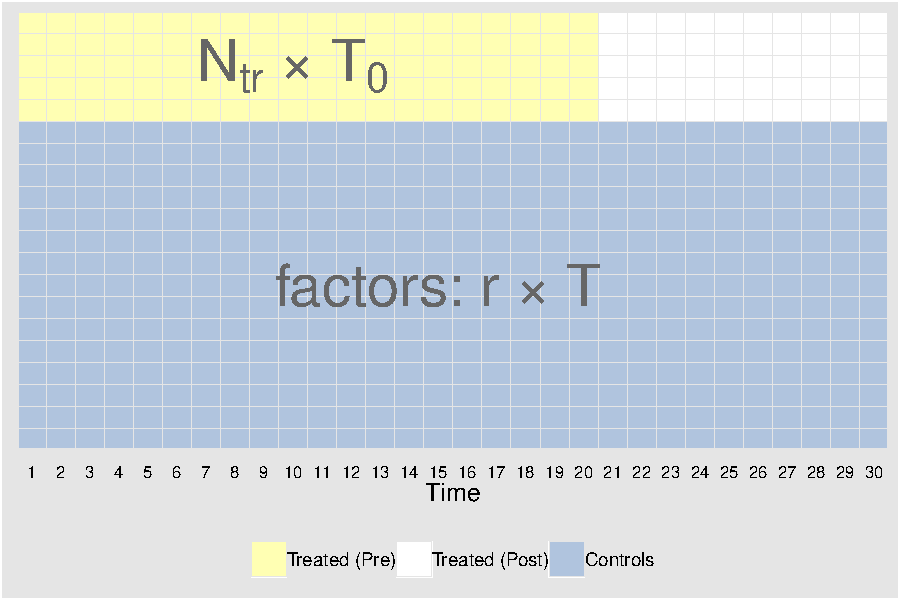
\includegraphics[width=\textwidth,height=1.75in,keepaspectratio]{sim_status4b.pdf}}%
\only<9>{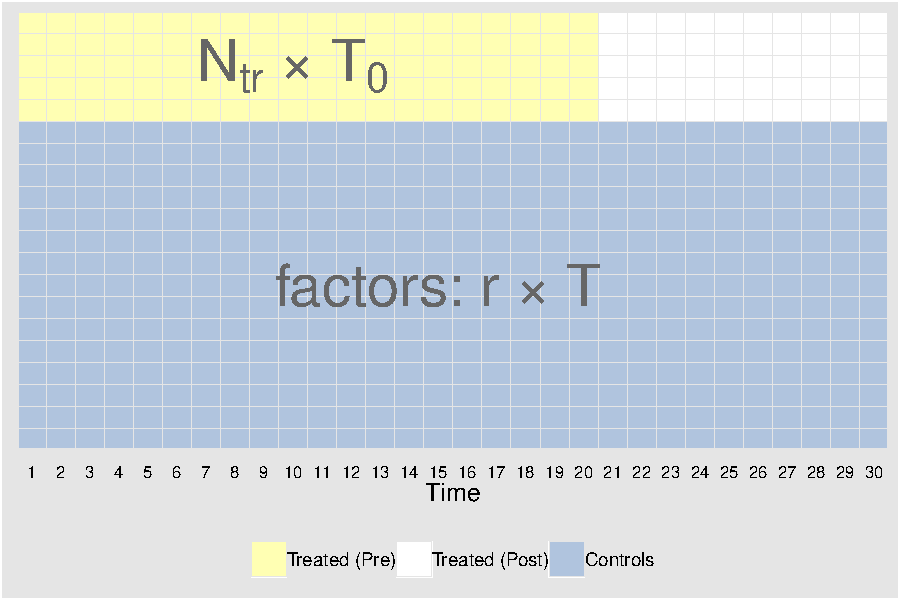
\includegraphics[width=\textwidth,height=1.75in,keepaspectratio]{sim_status4b.pdf}}%
\only<10->{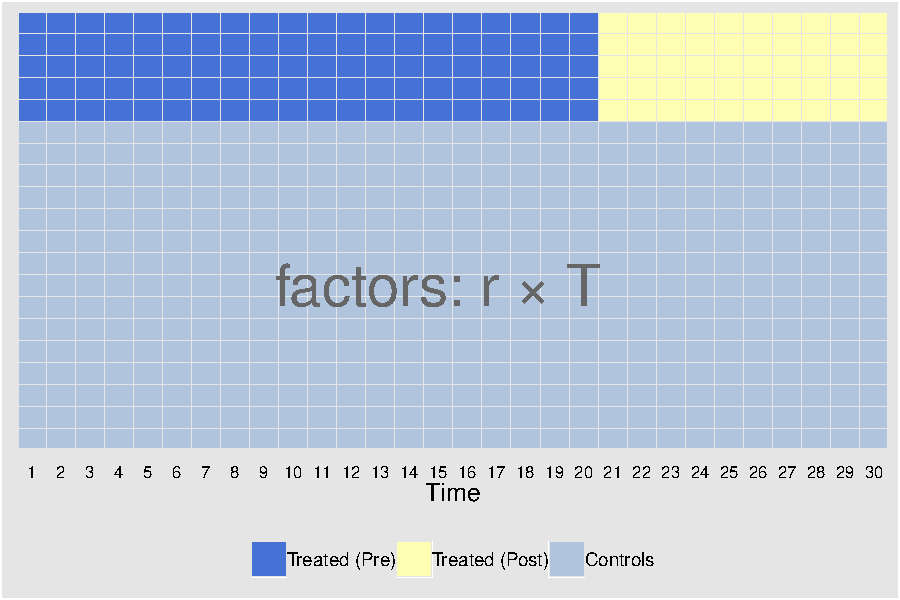
\includegraphics[width=\textwidth,height=1.75in,keepaspectratio]{sim_status5.pdf}}%
\end{column}
\end{columns}
\end{frame}
}
\else
{
\begin{frame}
 \frametitle{IFEct}
\vspace{1em}
\textcite{xu2017generalized} proposes a three-step approach based on a latent factor model:\vspace{-0.5em}
\begin{eqnarray*}
\mbox{\blue{Control }}\quad Y_{it}(0) &=& X_{it}'\beta + \alpha_{i}  + \xi_{t} + \lambda_{i}^{\prime} f_{t} + \varepsilon_{it} \\
\mbox{\blue{Treated}}\ \quad Y_{it}(0) &=& X_{it}'\beta + \alpha_{i}  + \xi_{t} + \lambda_{i}^{\prime} f_{t} + \varepsilon_{it}  \phantom{\hspace{3.2em}}\mbox{\blue{(pre)}} \\
Y_{it}(1) &=& X_{it}'\beta + \alpha_{i}  + \xi_{t} + \lambda_{i}^{\prime} f_{t} + \varepsilon_{it} + \tau_{it} \quad\mbox{\blue{(post)}}
\end{eqnarray*}\vspace{1em}
\vspace{-1em}
\begin{columns}[c]
% left column
\begin{column}{.45\textwidth}
\vspace{-2em}
\begin{enumerate}
\item Estimate using controls
\item Predict on treated $\widehat{Y}_{it}(0)$
\item Calculate the ATT
\item Expectation-Maximization\\{\footnotesize\blue{\parencite{gobillon2016regional}}}
\end{enumerate}
\end{column}
% right column
\begin{column}{.55\textwidth}
\vspace{-1em}
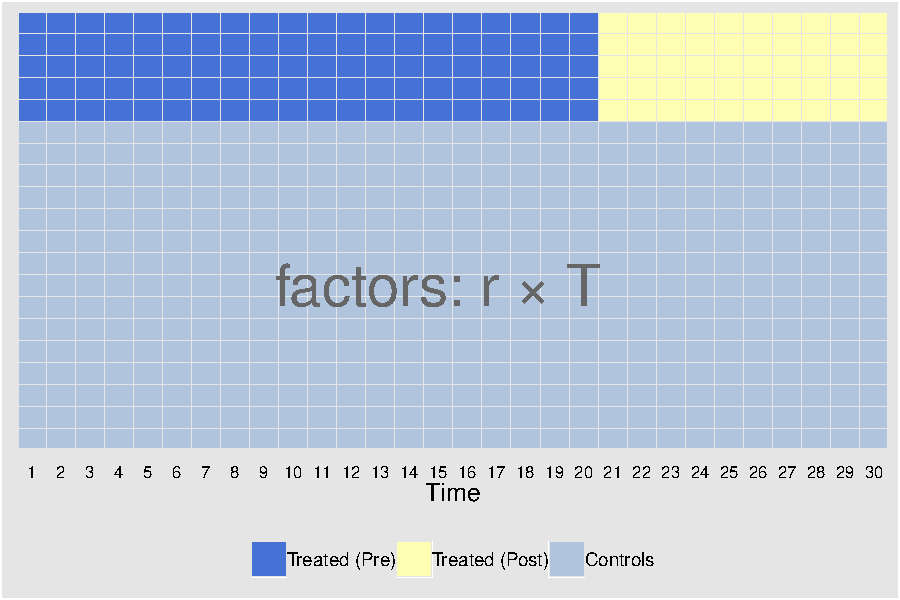
\includegraphics[width=\textwidth,height=1.75in,keepaspectratio]{sim_status5.pdf}%
\end{column}
\end{columns}
\end{frame}
}\fi

\if\handout0{
\begin{frame}
 \frametitle{Election Day Registration (EDR) and Voter Turnout}
\visible<4>{\vspace{-0.5em}
\begin{center}
\it\red{Causal inference is a missing data problem.}
\end{center}\vspace{-1em}
}
\only<1>{
\vspace{-2em}
\begin{center}
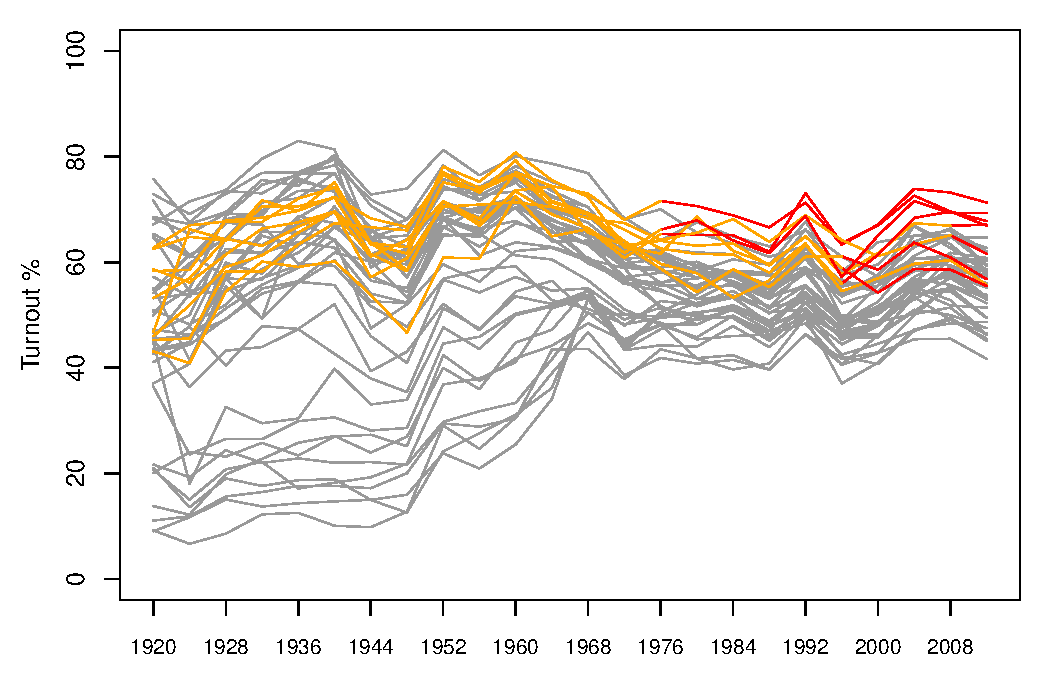
\includegraphics[width=.9\textwidth,height=2.45in,keepaspectratio]{edr_rawdata.pdf}
\end{center}
}%
\only<2>{
\vspace{-2em}
\begin{center}
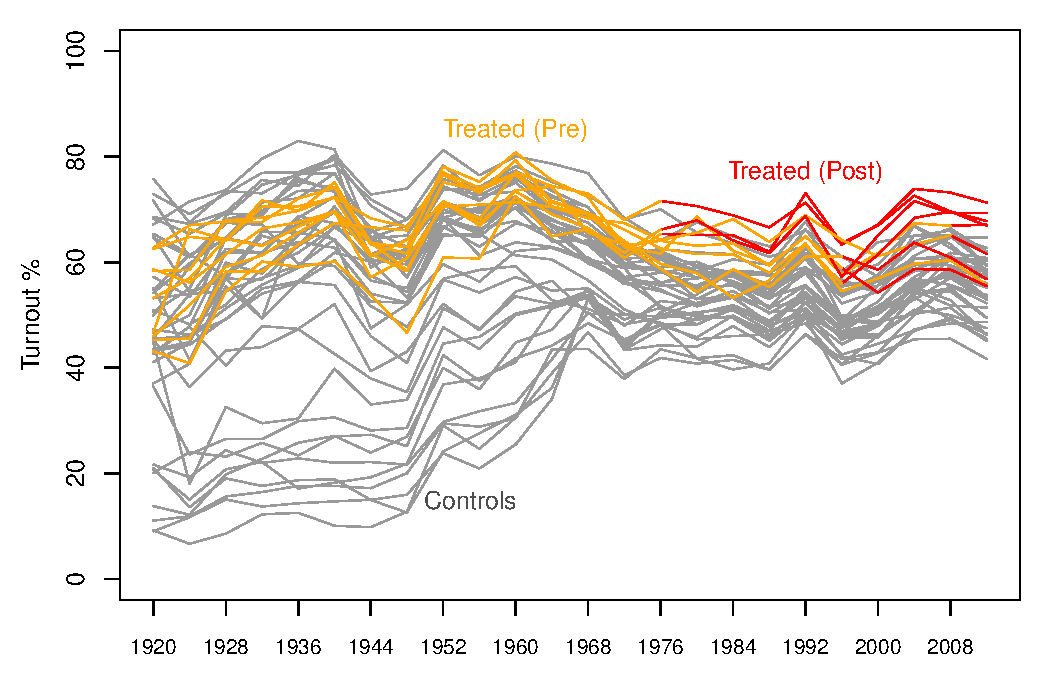
\includegraphics[width=.9\textwidth,height=2.45in,keepaspectratio]{edr_rawdata2.pdf}
\end{center}
\vspace{-1em}
}%
\only<3>{\centering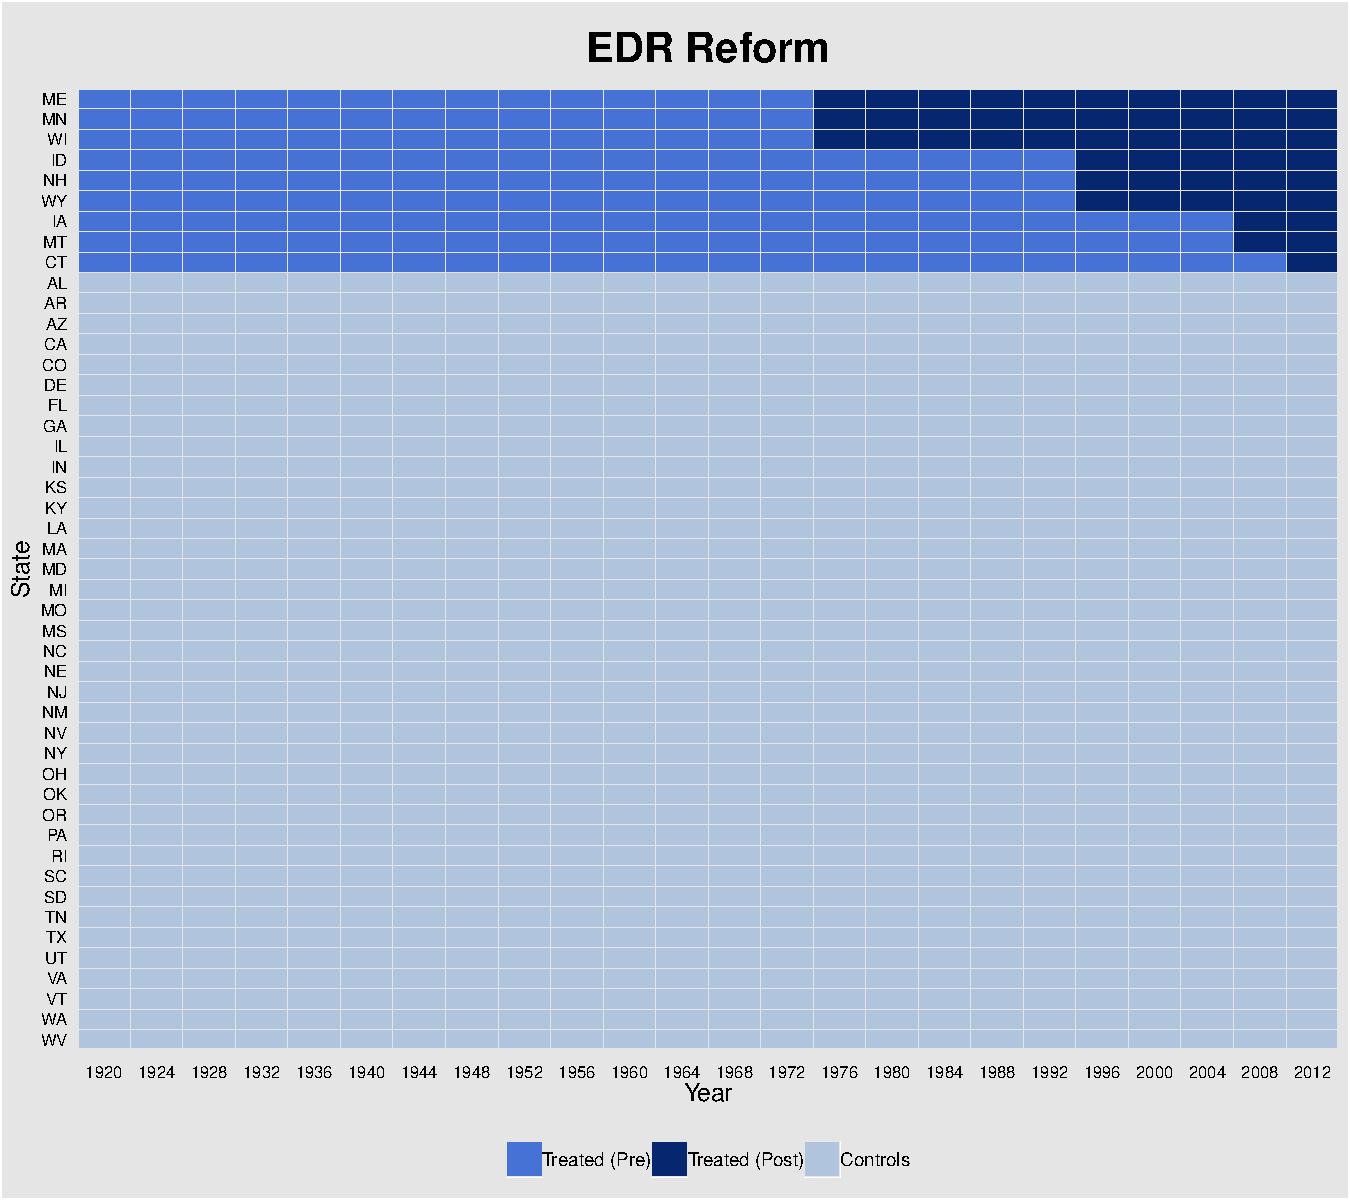
\includegraphics[height=2.45in,keepaspectratio]{edr_status.pdf}}%
\only<4->{\centering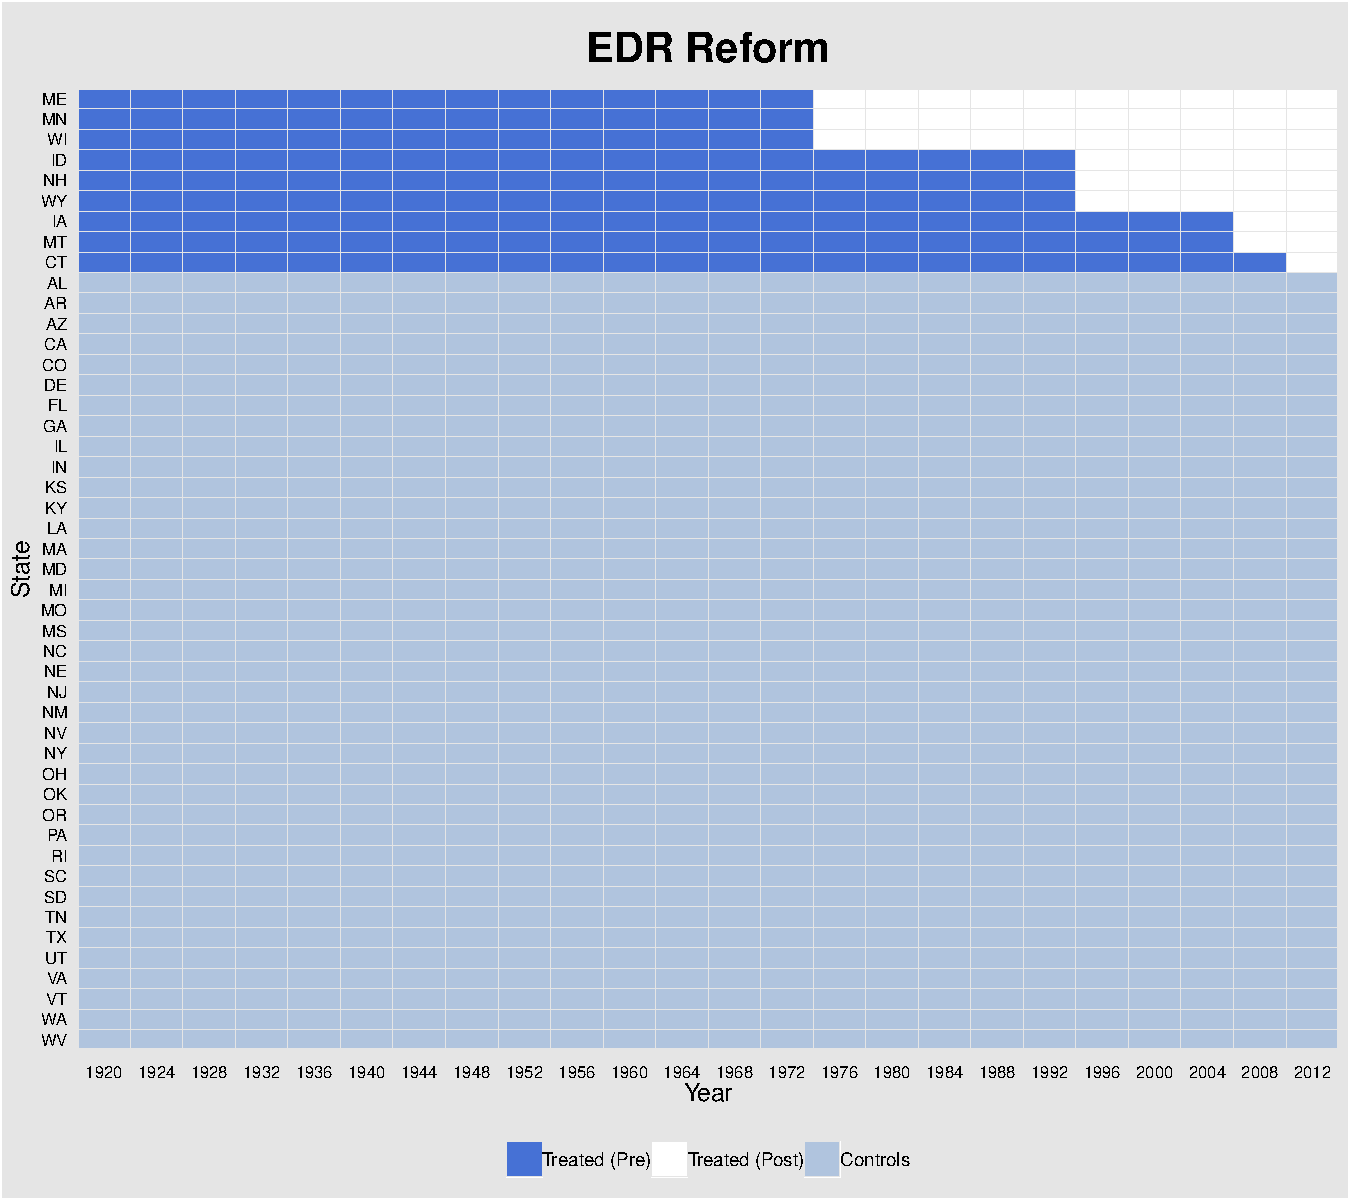
\includegraphics[height=2.45in,keepaspectratio]{edr_status2.pdf}}%
\end{frame}
}\else{
\begin{frame}
 \frametitle{Election Day Registration (EDR) and Voter Turnout}
\vspace{-0.5em}
\begin{center}
\it\red{Causal inference is a missing data problem.}
\end{center}\vspace{-1em}
\centering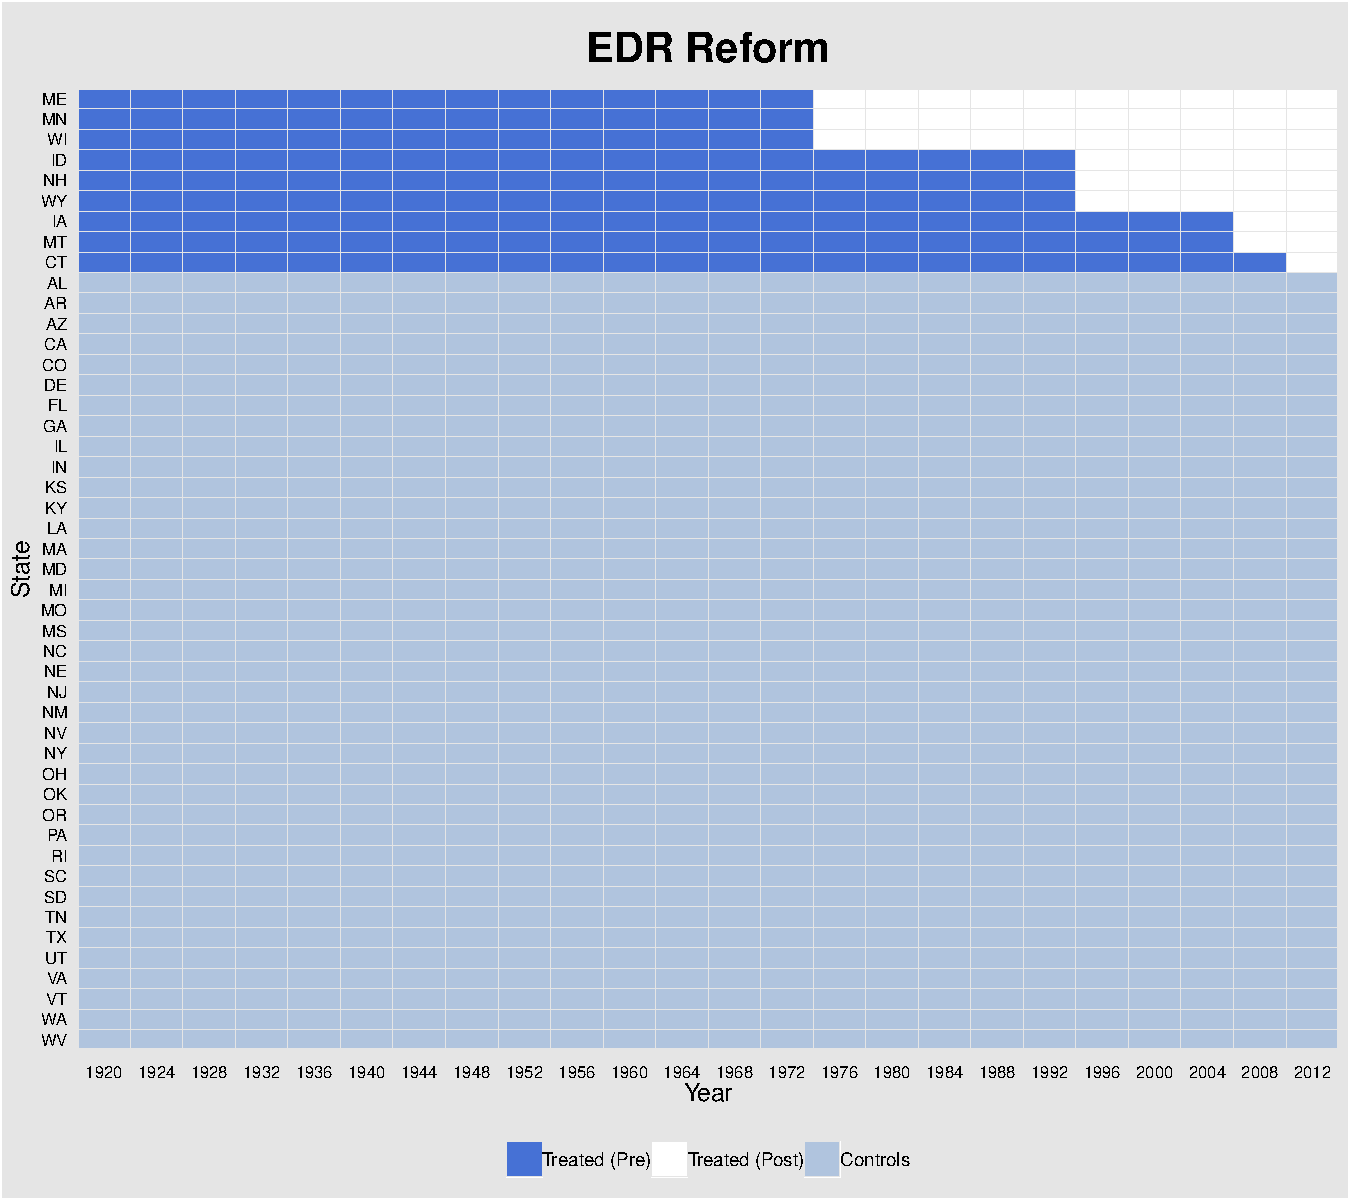
\includegraphics[height=2.45in,keepaspectratio]{edr_status2.pdf}%
\end{frame}
}\fi

\if\handout0{
\begin{frame}
\only<1-2>{\frametitle{The Case of Connecticut}}%
\only<3-4>{\frametitle{The Case of New Hampshire}}%
\only<5->{\frametitle{Main Results}}%
% Connecticut
\only<1>{
\centering%
Difference-in-Differences\\\vspace{0.2em}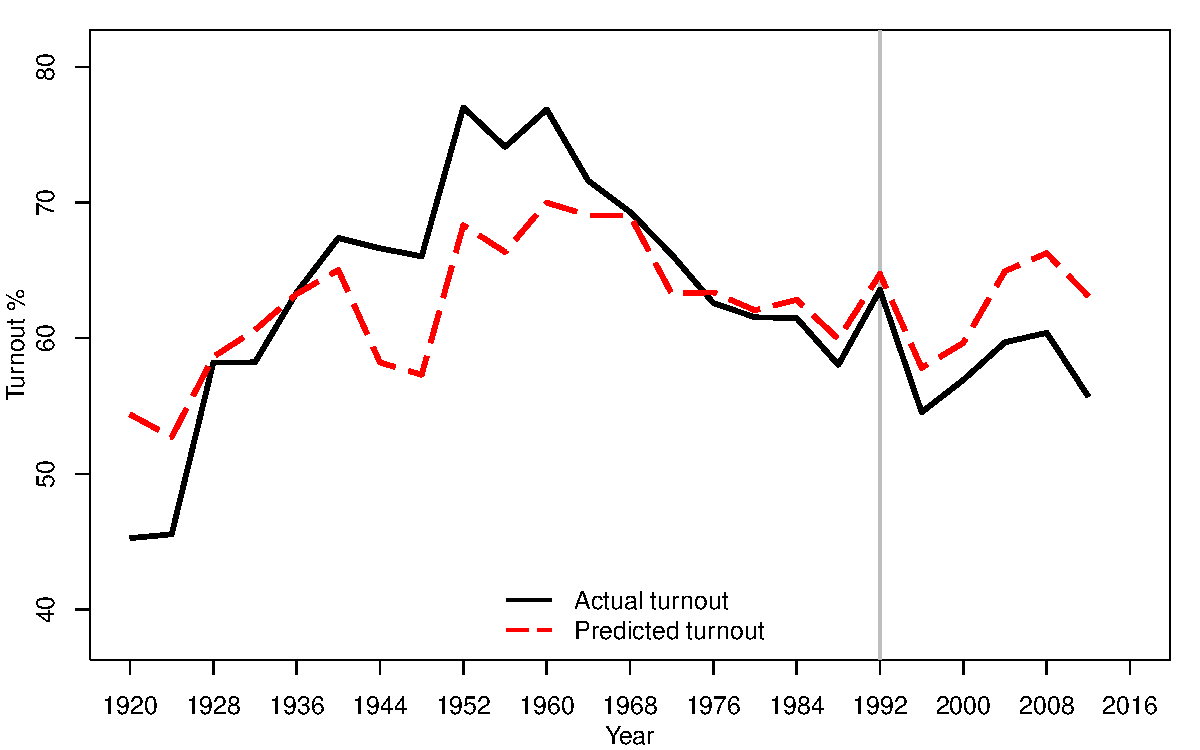
\includegraphics[height=2.25in,keepaspectratio]{edr_case_ct1.pdf}%
}%
\only<2>{
\centering%
\blue{IFEct} with Two Factors\\\vspace{0.2em}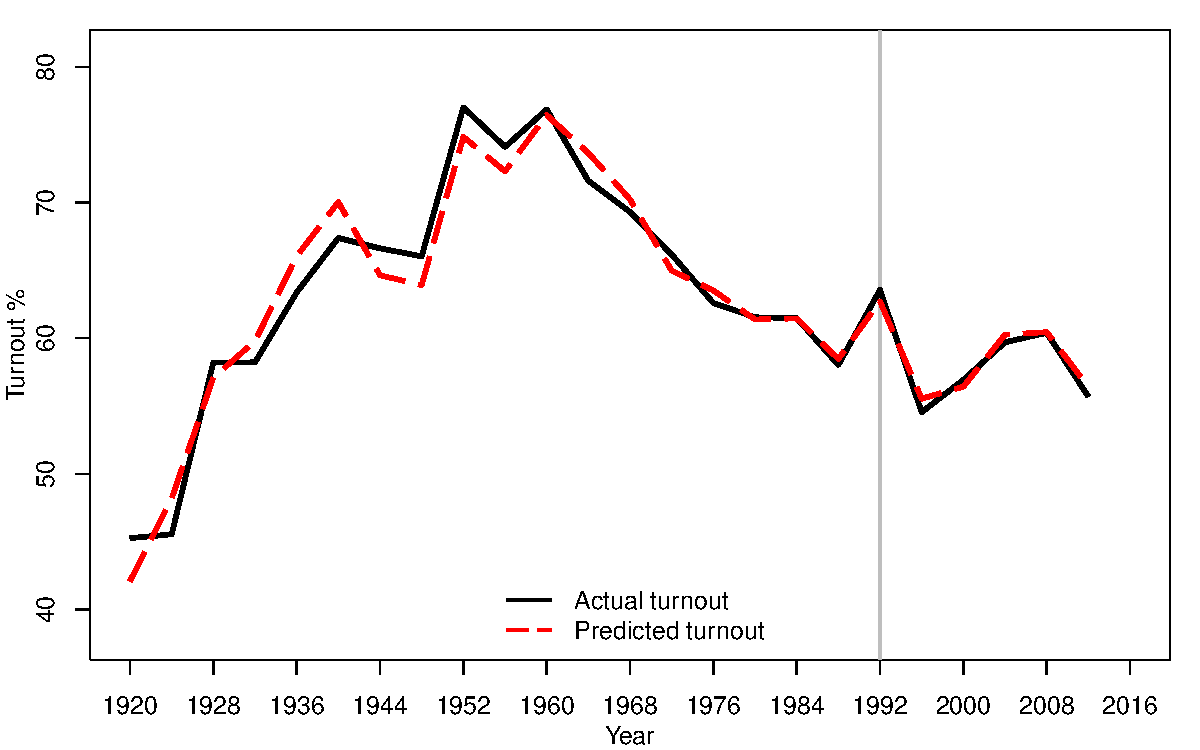
\includegraphics[height=2.25in,keepaspectratio]{edr_case_ct2.pdf}%
}%
% new Hampshire
\only<3>{
\centering%
Difference-in-Differences\\\vspace{0.2em}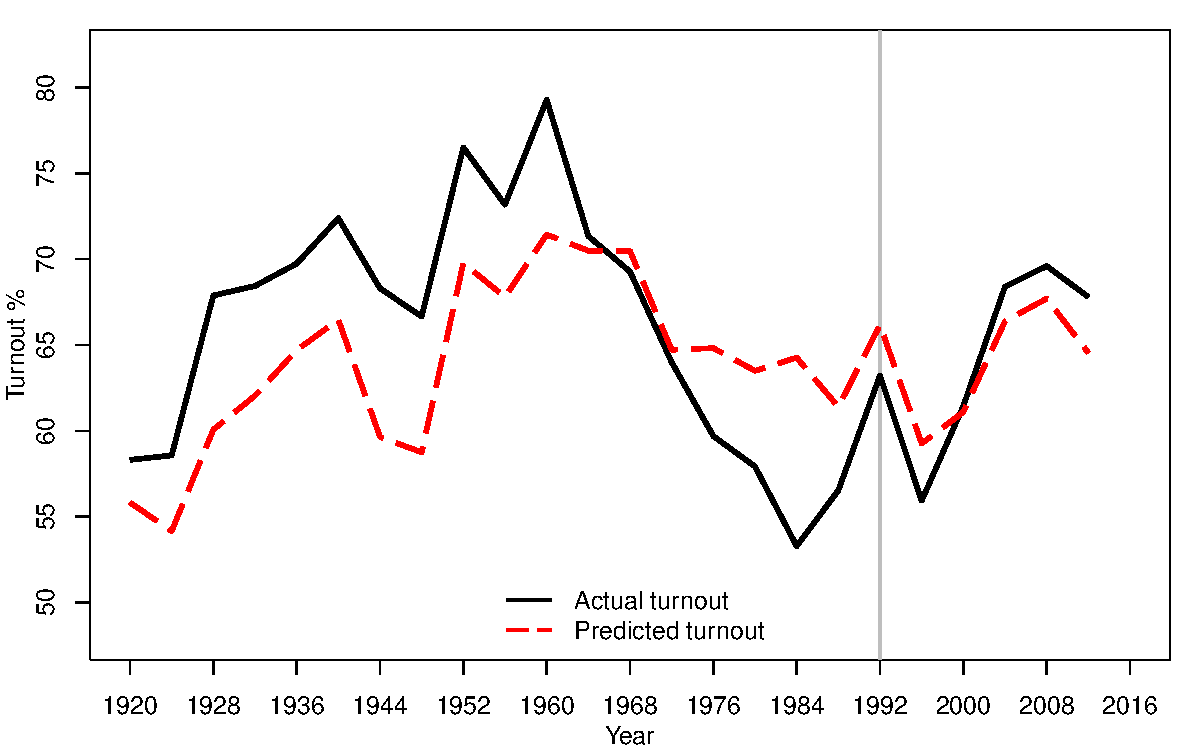
\includegraphics[height=2.25in,keepaspectratio]{edr_case_nh1.pdf}%
}%
\only<4>{
\centering%
\blue{IFEct} with Two Factors\\\vspace{0.2em}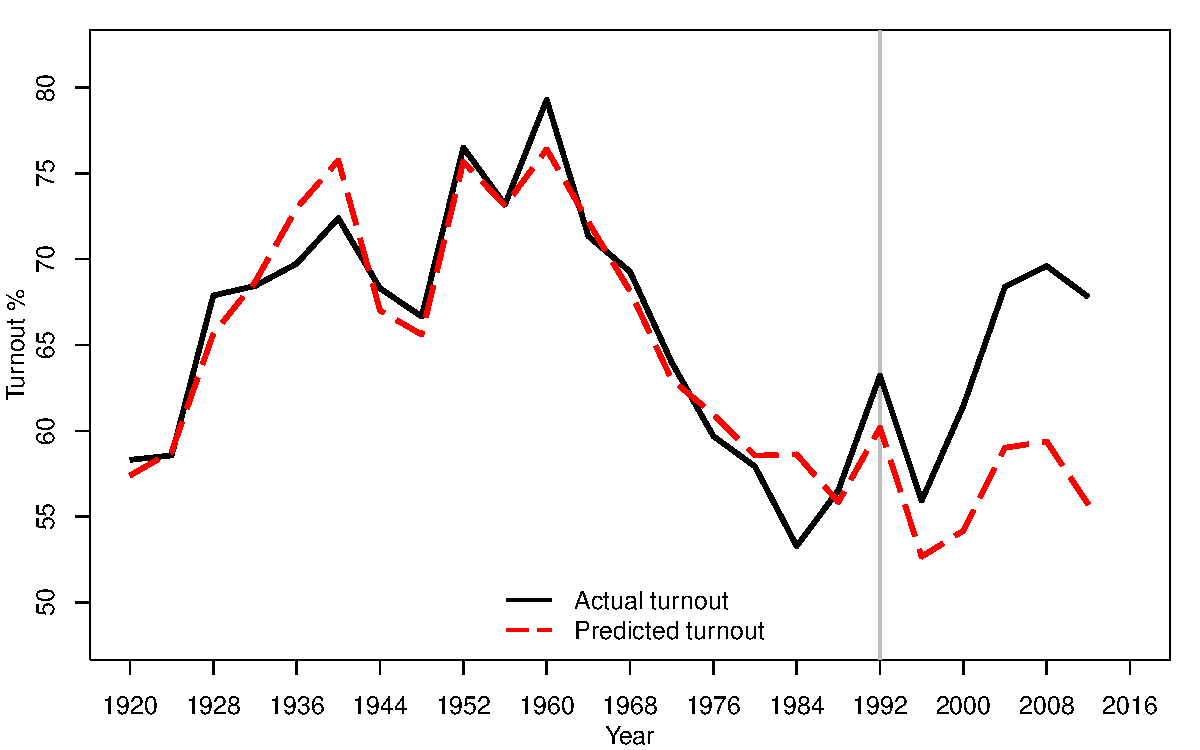
\includegraphics[height=2.25in,keepaspectratio]{edr_case_nh2.pdf}%
}%
% average. Was \only<6->, while the frametitle above switches at <5->, so overlay 5
% rendered as a titled blank slide. Now both fire together.
\only<5->{
\begin{adjustwidth}{-2em}{-2em}
\vspace{1em}
\begin{center}
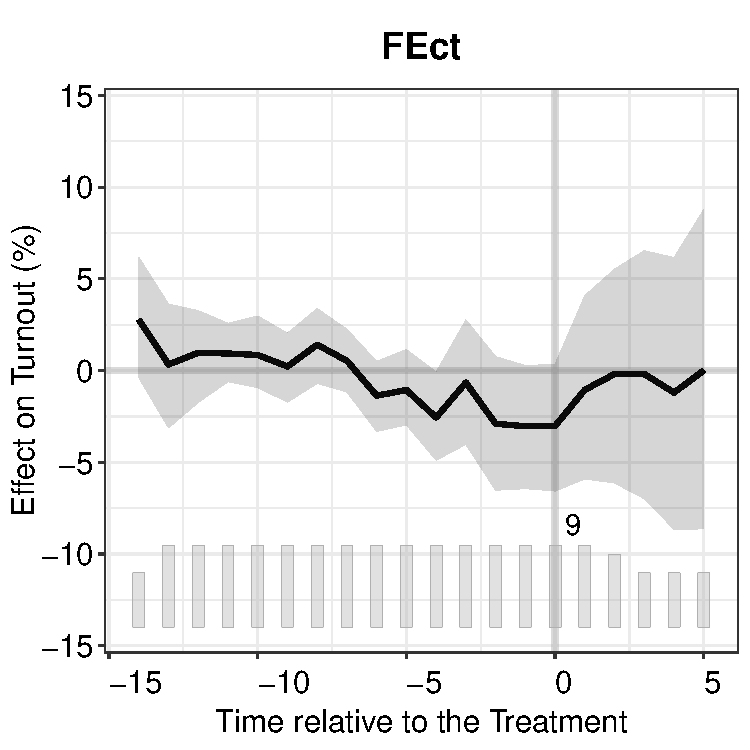
\includegraphics[width=0.48\textwidth,height=2.3in,keepaspectratio]{xu2017_fect.pdf}\hspace{1em}
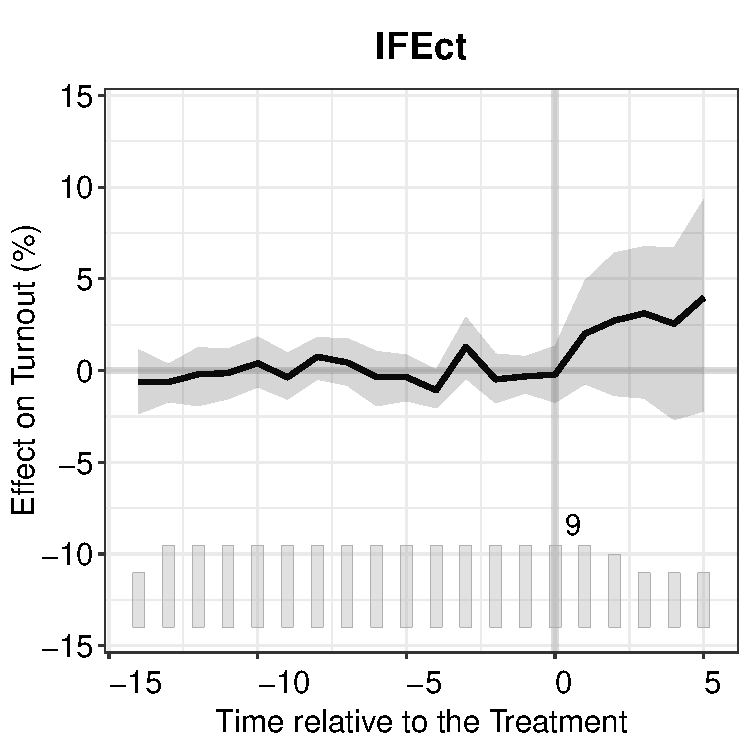
\includegraphics[width=0.48\textwidth,height=2.3in,keepaspectratio]{xu2017_ifect.pdf}
\end{center}
\end{adjustwidth}
}
\end{frame}
}
\else{
\begin{frame}
\frametitle{Main Results}%
\begin{adjustwidth}{-2em}{-2em}
\vspace{1em}
\begin{center}
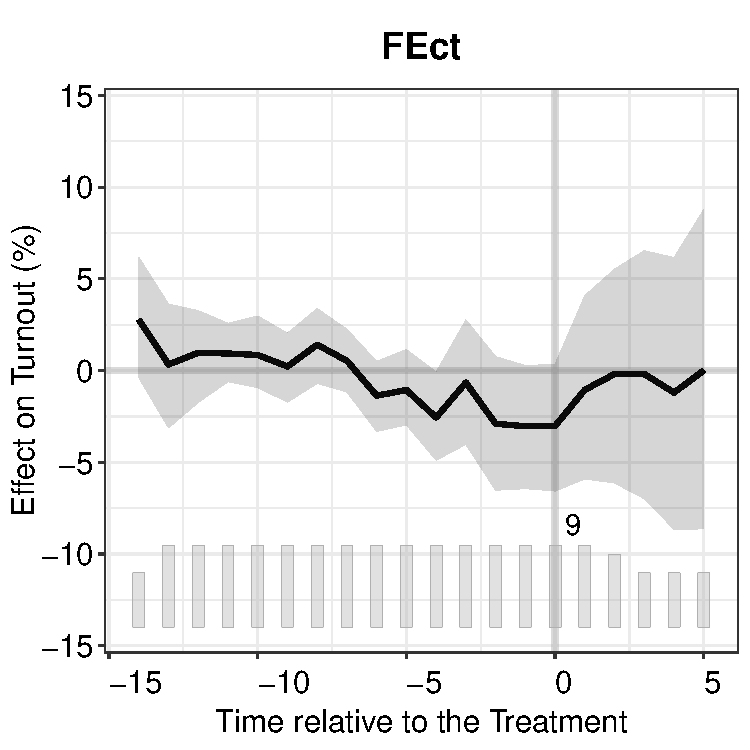
\includegraphics[width=0.48\textwidth,height=2.3in,keepaspectratio]{xu2017_fect.pdf}\hspace{1em}
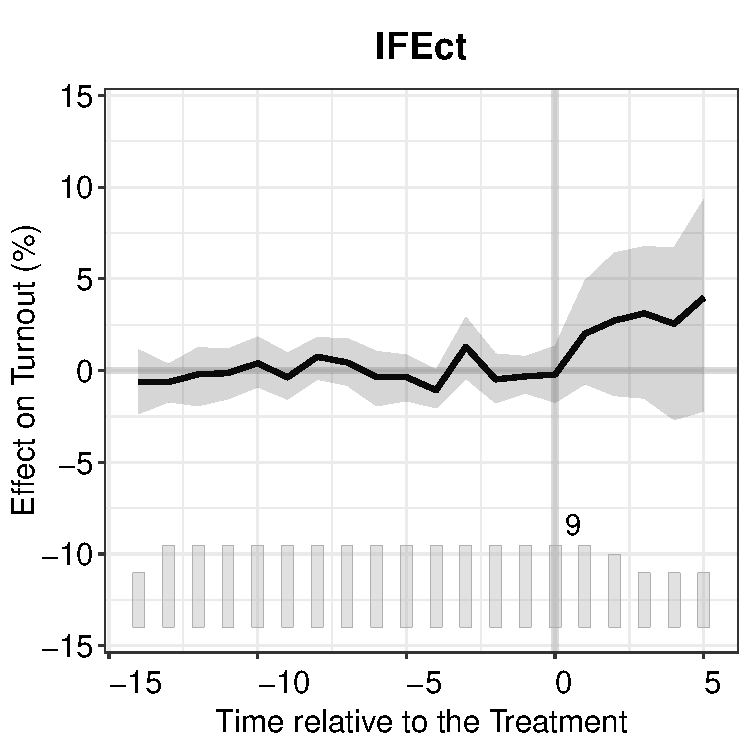
\includegraphics[width=0.48\textwidth,height=2.3in,keepaspectratio]{xu2017_ifect.pdf}
\end{center}
\end{adjustwidth}
\end{frame}
}\fi

\if\handout0{
\begin{frame}[c]
 \frametitle{Factors and Factor Loadings}
\begin{center}
\only<1,3>{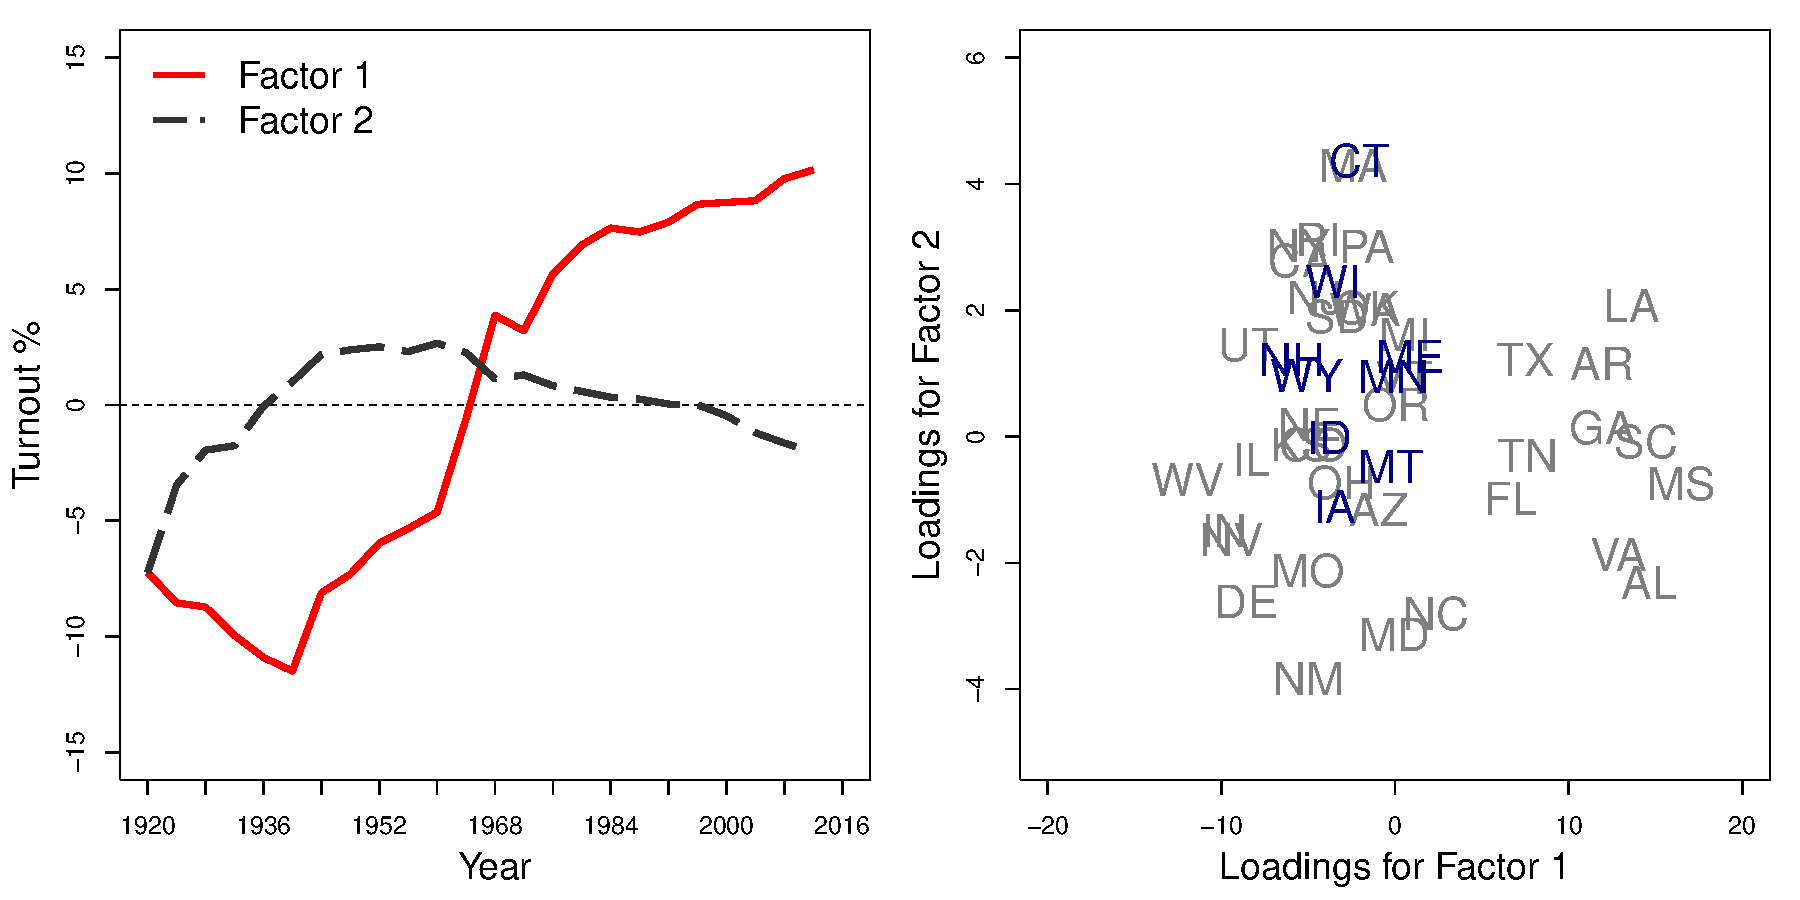
\includegraphics[width=\textwidth,height=2.45in,keepaspectratio]{edr_FL.pdf}}%
\only<2>{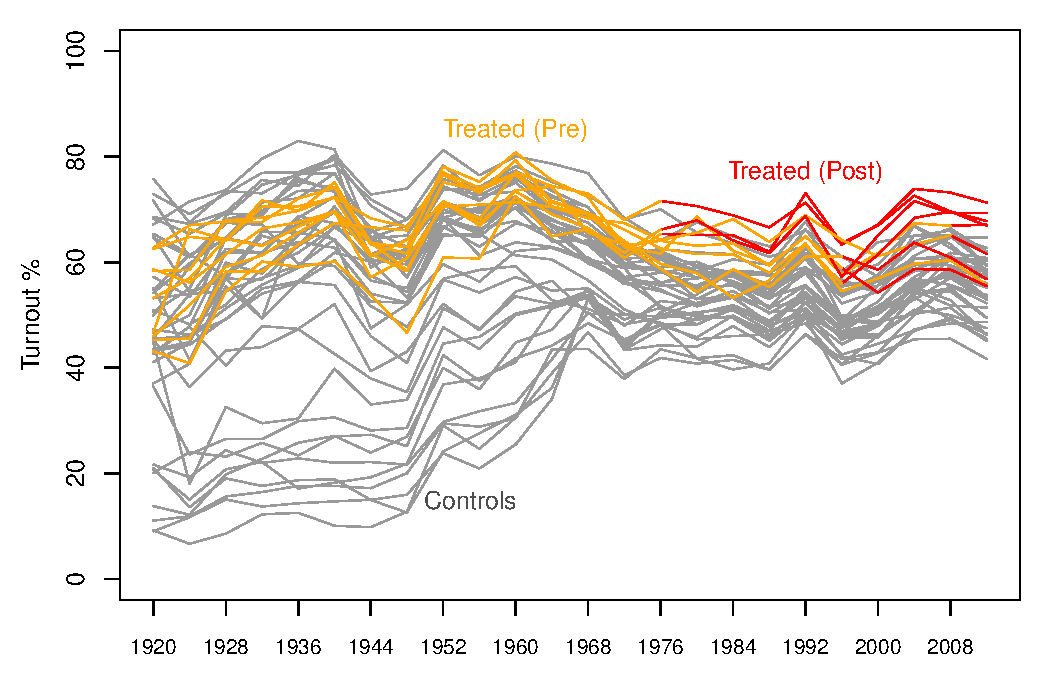
\includegraphics[width=.9\textwidth,height=2.45in,keepaspectratio]{edr_rawdata2.pdf}}%
\only<4>{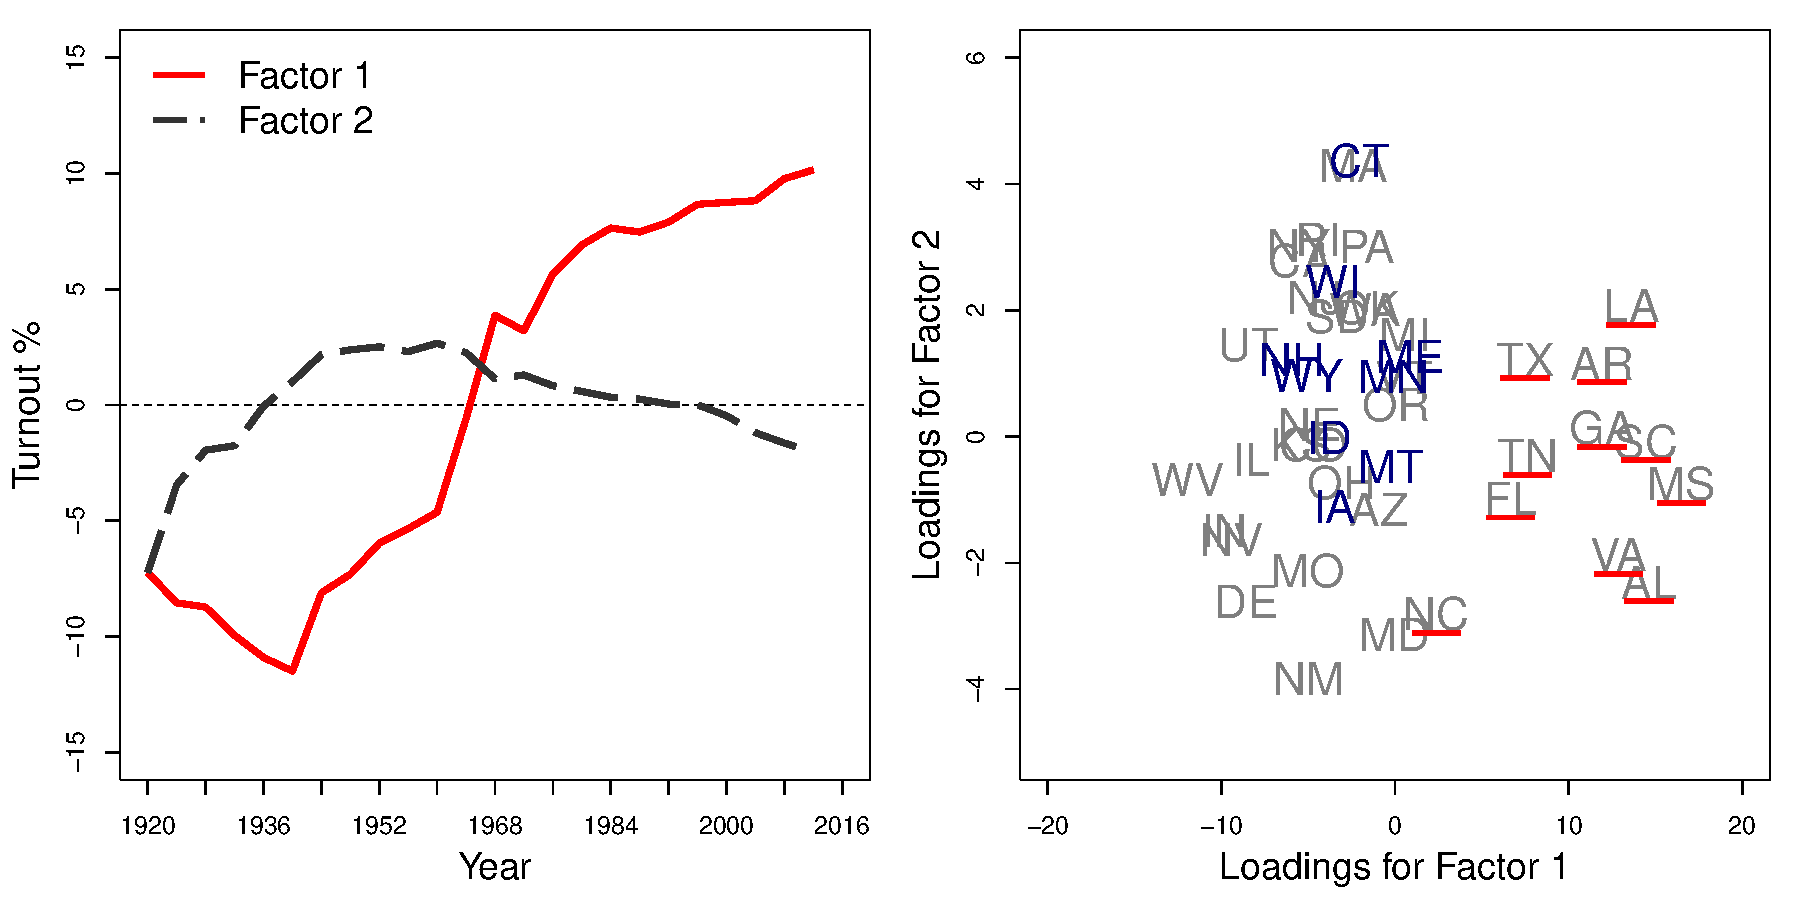
\includegraphics[width=\textwidth,height=2.45in,keepaspectratio]{edr_FL2.pdf}}%
\end{center}
\end{frame}
}\else{
\begin{frame}[c]
 \frametitle{Factors and Factor Loadings}
\begin{center}
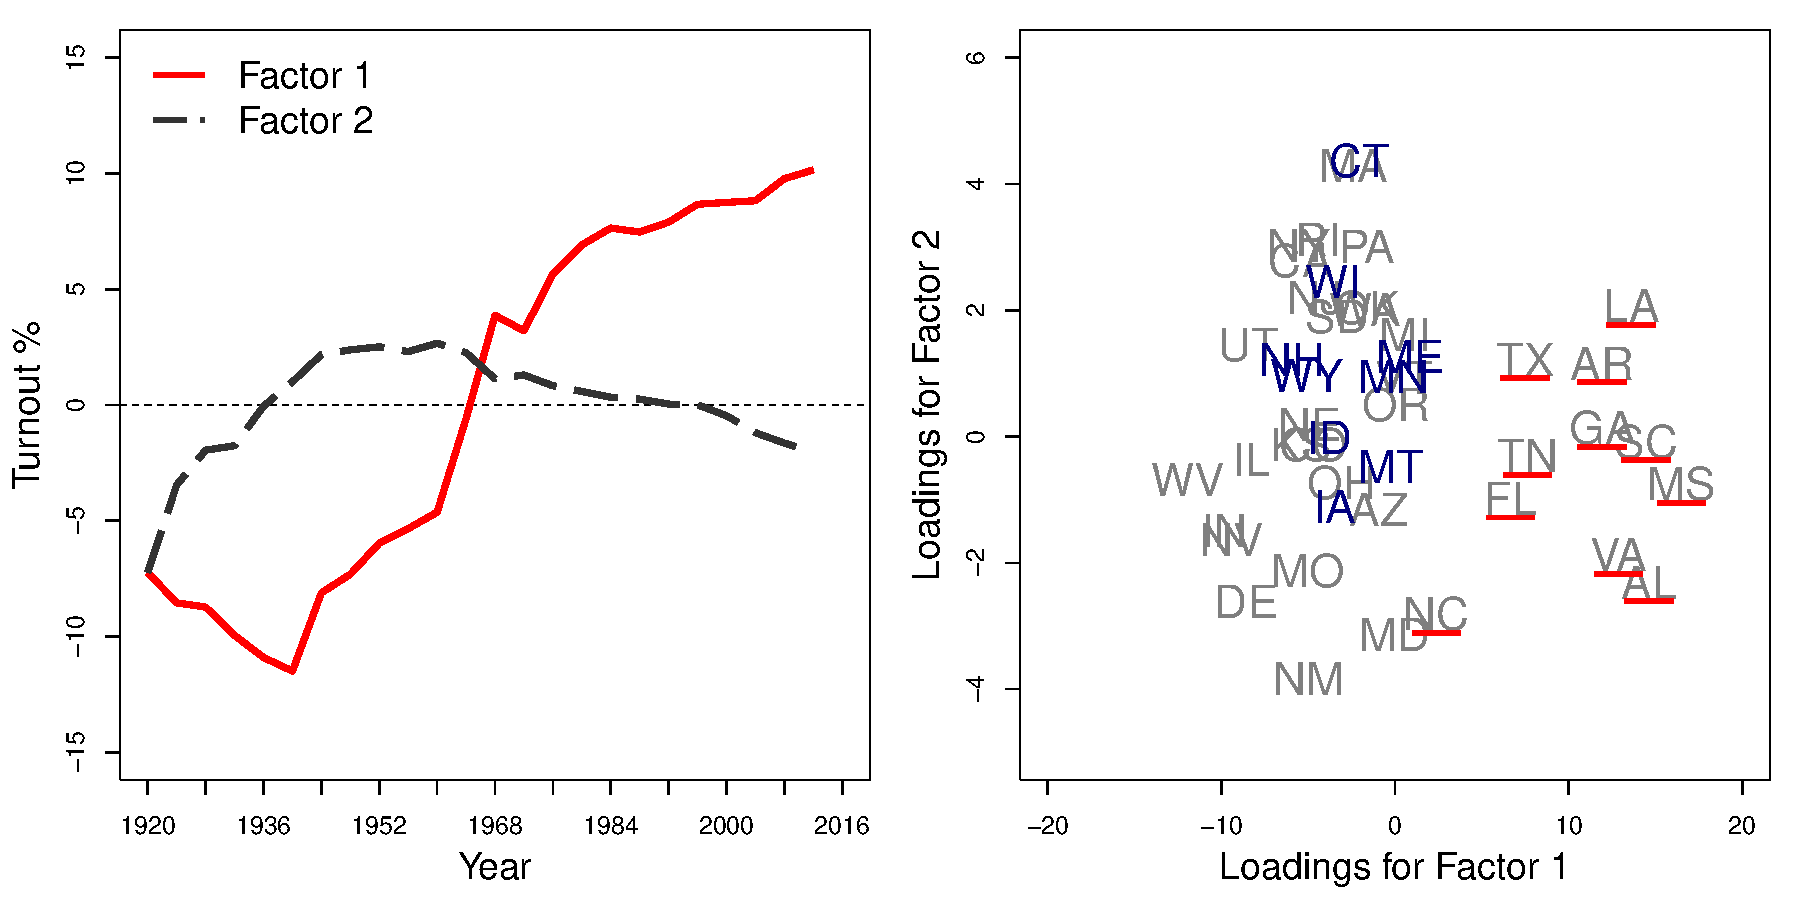
\includegraphics[width=\textwidth,height=2.45in,keepaspectratio]{edr_FL2.pdf}%
\end{center}
\end{frame} 
}\fi

\begin{frame}[c]
 \frametitle{Placebo Test}
\begin{center}
\visible<1->{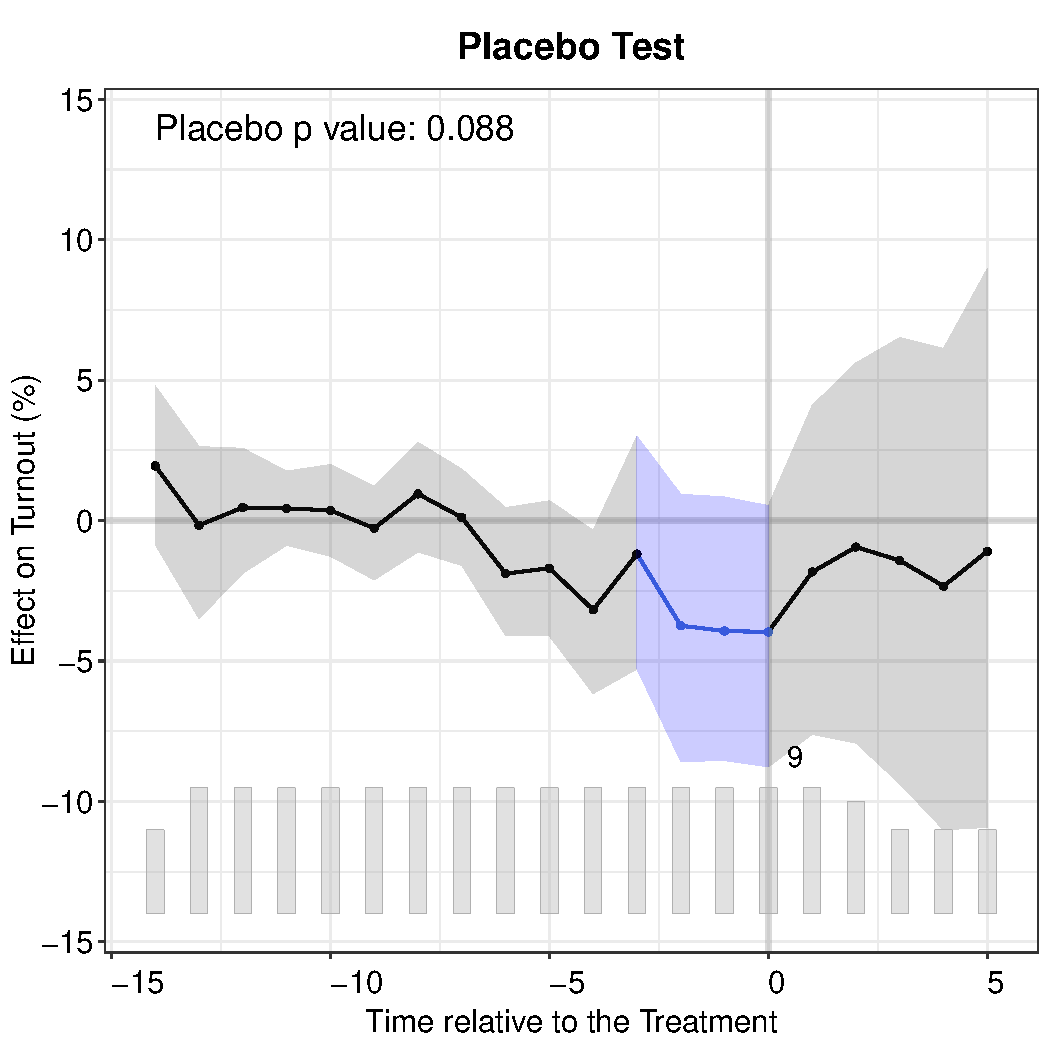
\includegraphics[width=0.45\textwidth]{ex_Xu2017_fect_3.pdf}}%
\hspace{2em}
\visible<2->{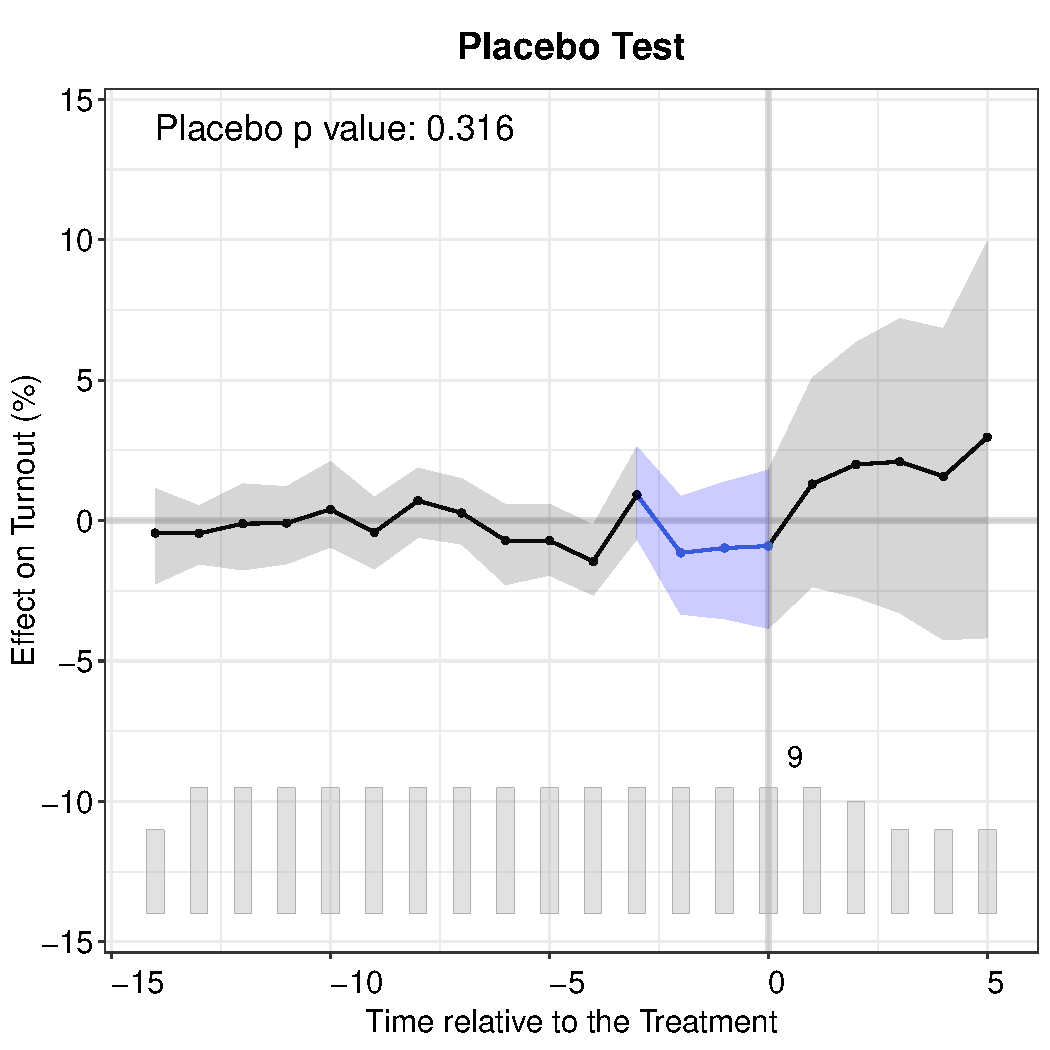
\includegraphics[width=0.45\textwidth]{ex_Xu2017_ife_2.pdf}}%
\end{center}
\end{frame}


\begin{frame}
\frametitle{Example: Property Rights and Land Improvement}
\blue{\small \textcite{sanford2019geospatial}}
\begin{itemize}
\item Do property rights lead to improved land quality? \pause
\item ``Experiment'': giving peasants in Borgou, Benin land titles\pause
\item Use satellite (remote sensing) data to measure land improvement, i.e., switch from annual crops to perennial crops (bushes and trees)\pause
\item Use IFEct to construct counterfactuals\pause
\end{itemize}
\begin{center}
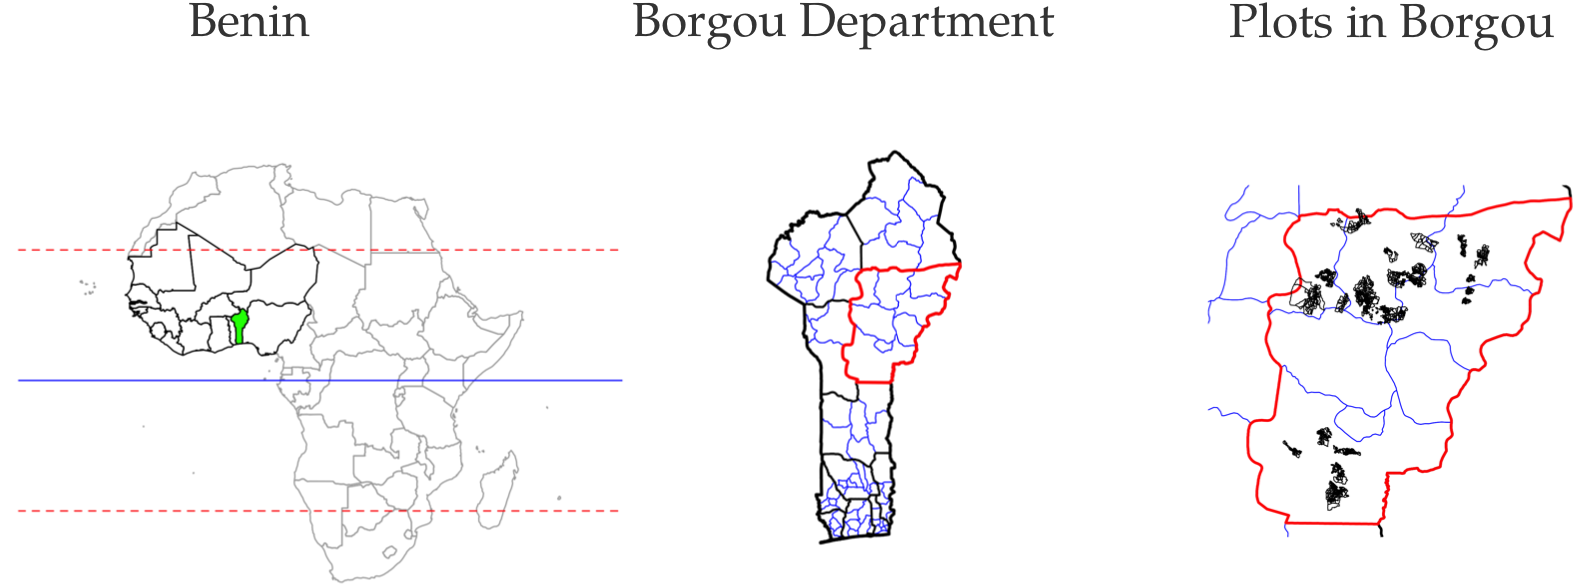
\includegraphics[width=0.6\textwidth]{benin_smp.png}
\end{center}
\end{frame}

\begin{frame}[c]
\frametitle{Original Satellite Images}
\begin{center}
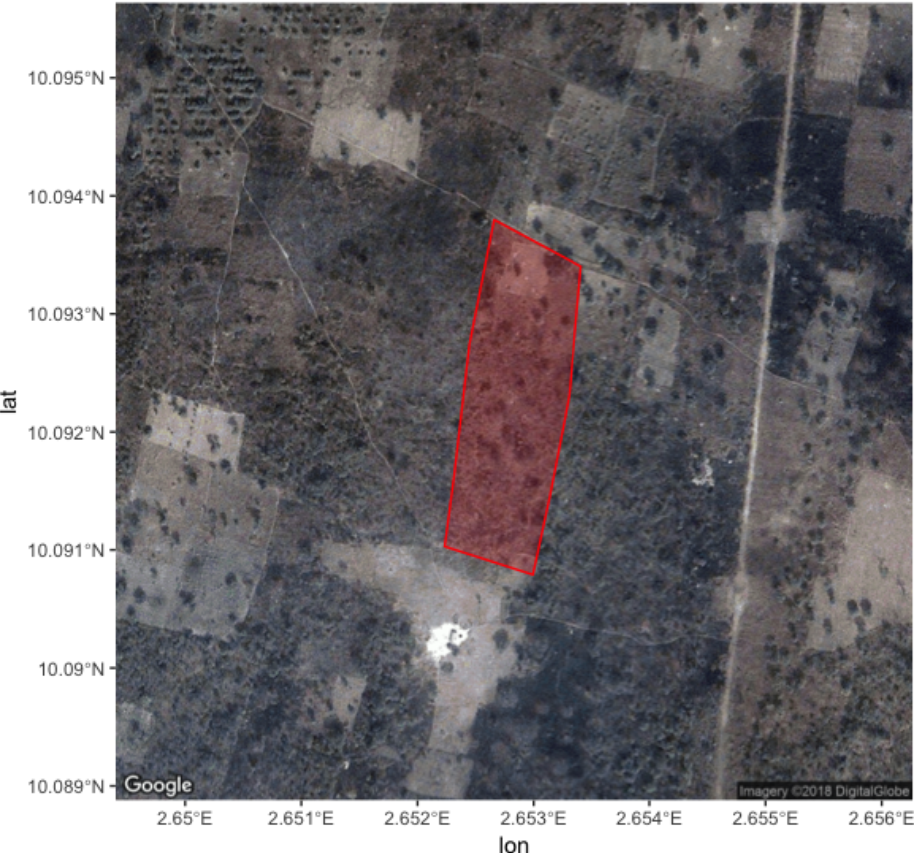
\includegraphics[width=0.45\textwidth]{benin_data1.png}\hspace{2em}
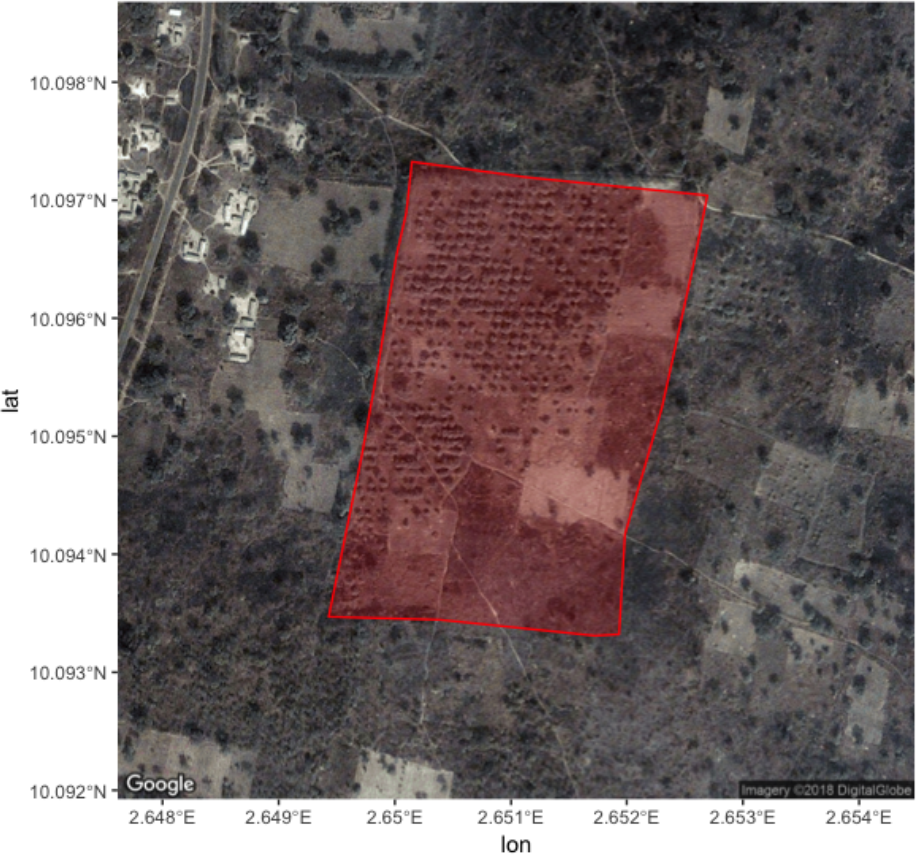
\includegraphics[width=0.45\textwidth]{benin_data2.png}
\end{center}
\end{frame}

\begin{frame}[c]
\frametitle{Treated and Counterfactual Averages}
\begin{center}
Pre-treatment Outcome\\ 
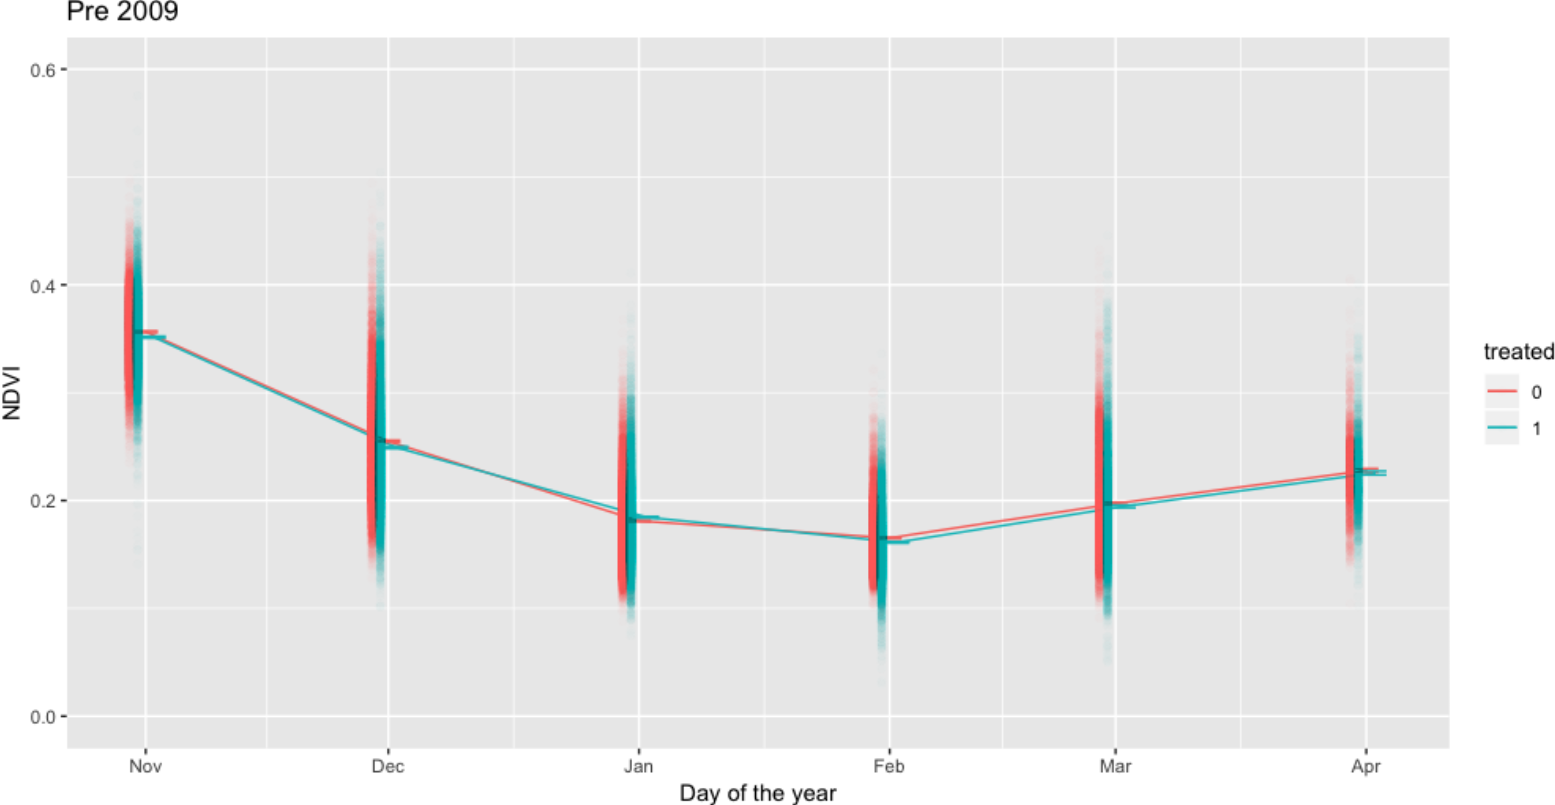
\includegraphics[width=0.8\textwidth]{benin_2009.png}
\end{center}
\end{frame}


\begin{frame}[c]
\frametitle{Treated and Counterfactual Averages}
\begin{center}
Post-treatment Outcome (4 Years)\\ 
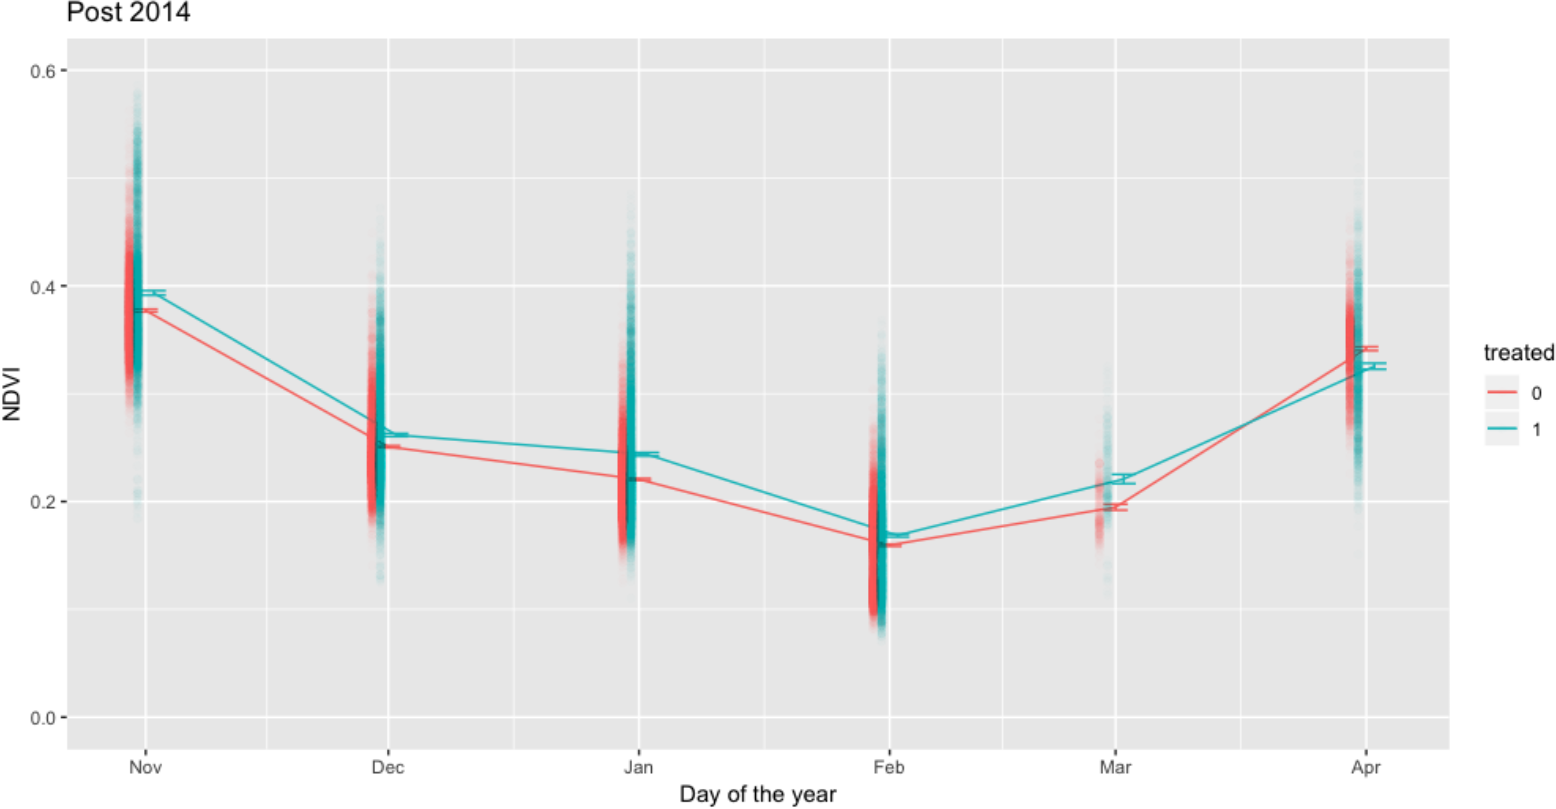
\includegraphics[width=0.8\textwidth]{benin_2014.png}
\end{center}
\end{frame}


\if\handout0{
\begin{frame}[c]
\frametitle{Matrix Completion Methods}
\begin{columns}
\begin{column}{0.5\textwidth}
  \vspace{-1em}
  \begin{center}
  \only<1,2>{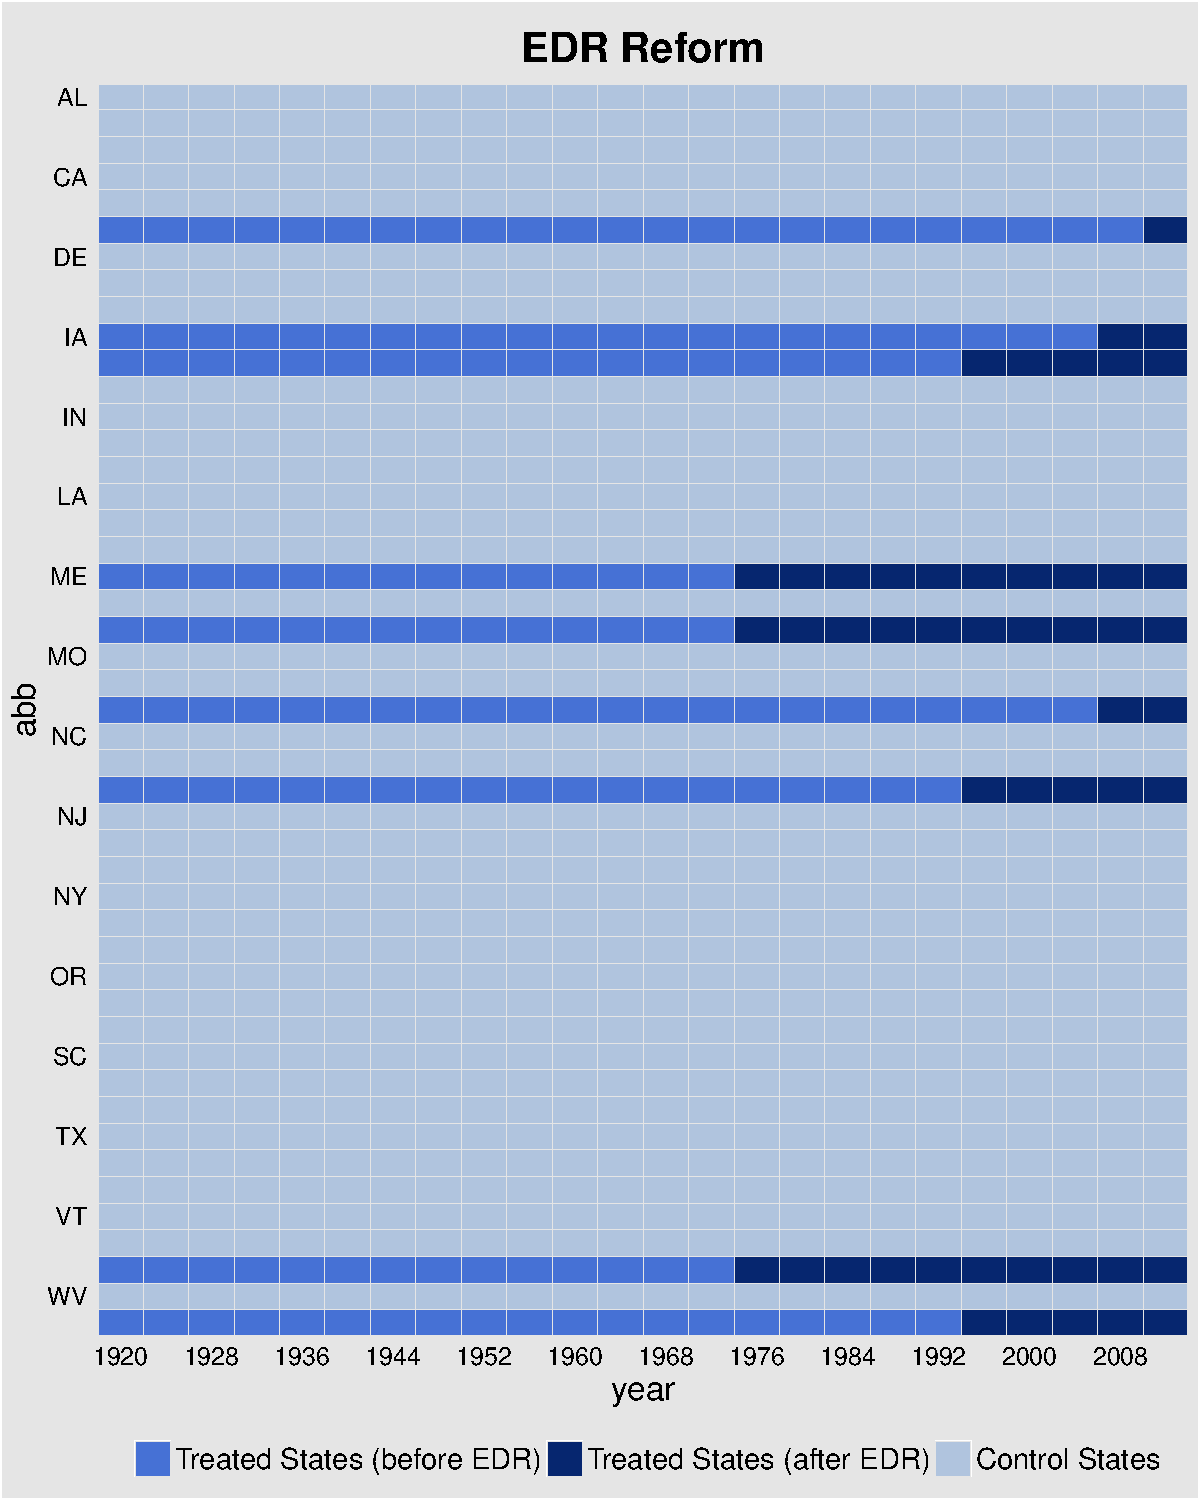
\includegraphics[height=0.8\textheight]{edr_missing0.pdf}}%
  \only<3-4>{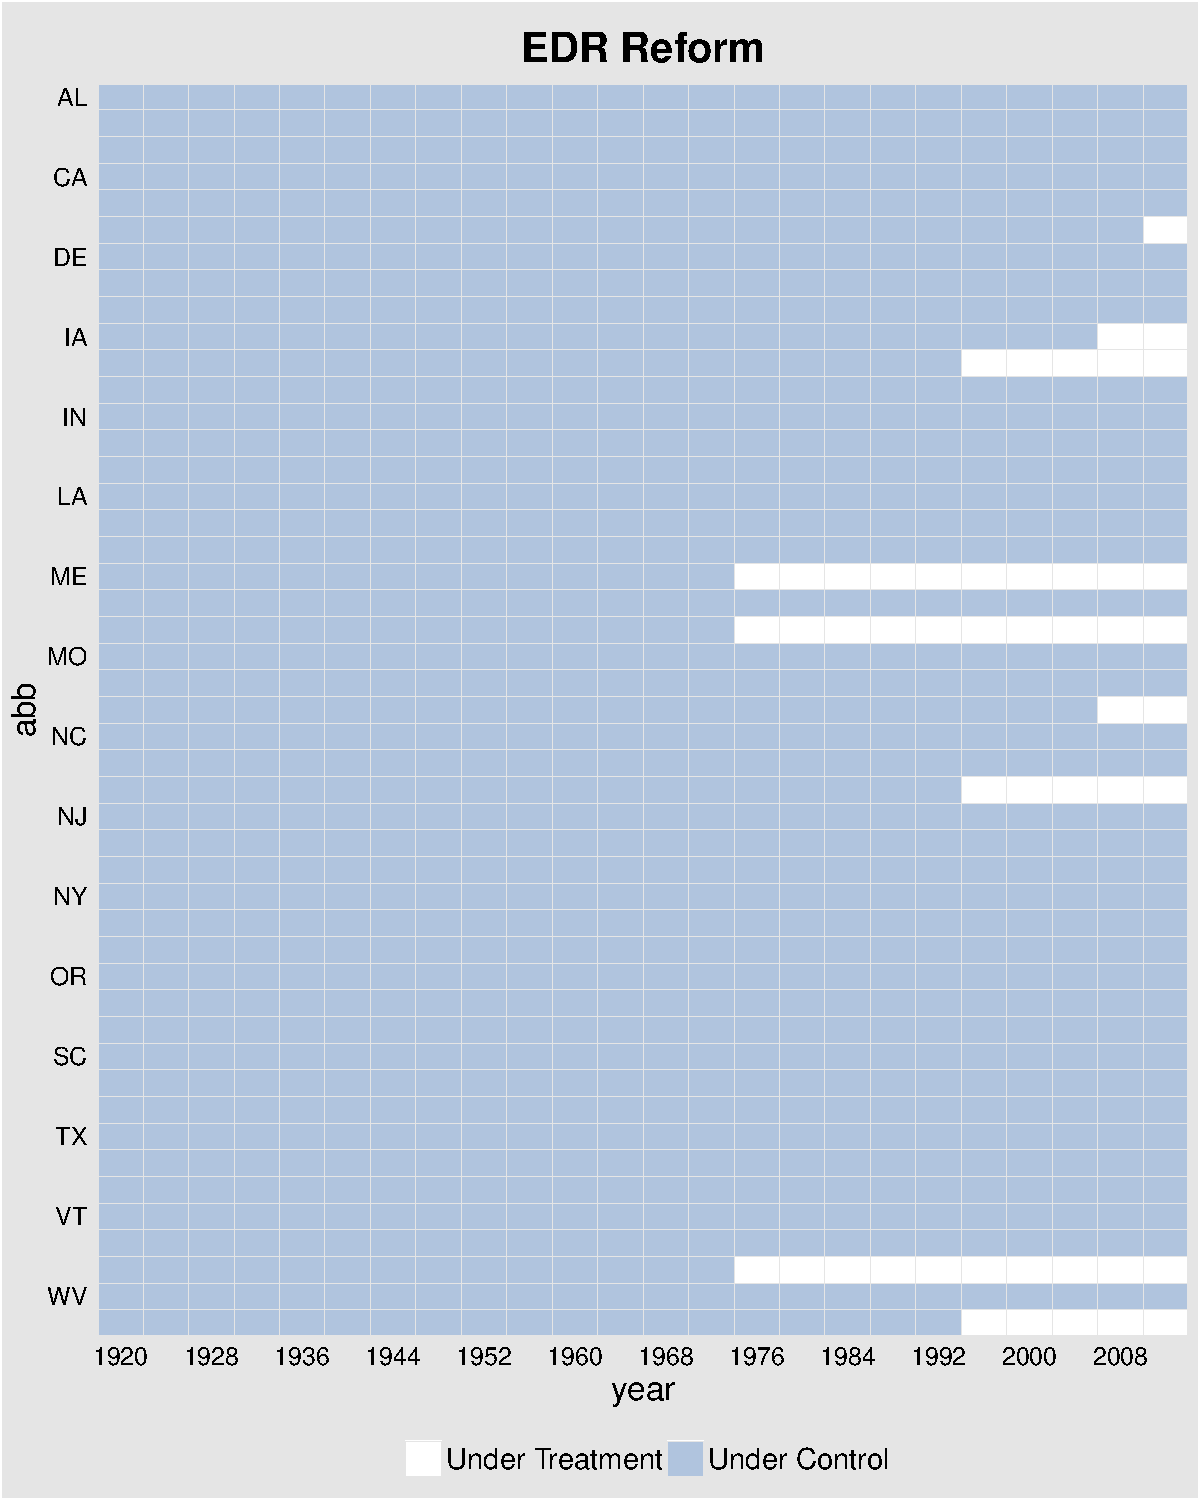
\includegraphics[height=0.8\textheight]{edr_missing2.pdf}}%
  \only<5->{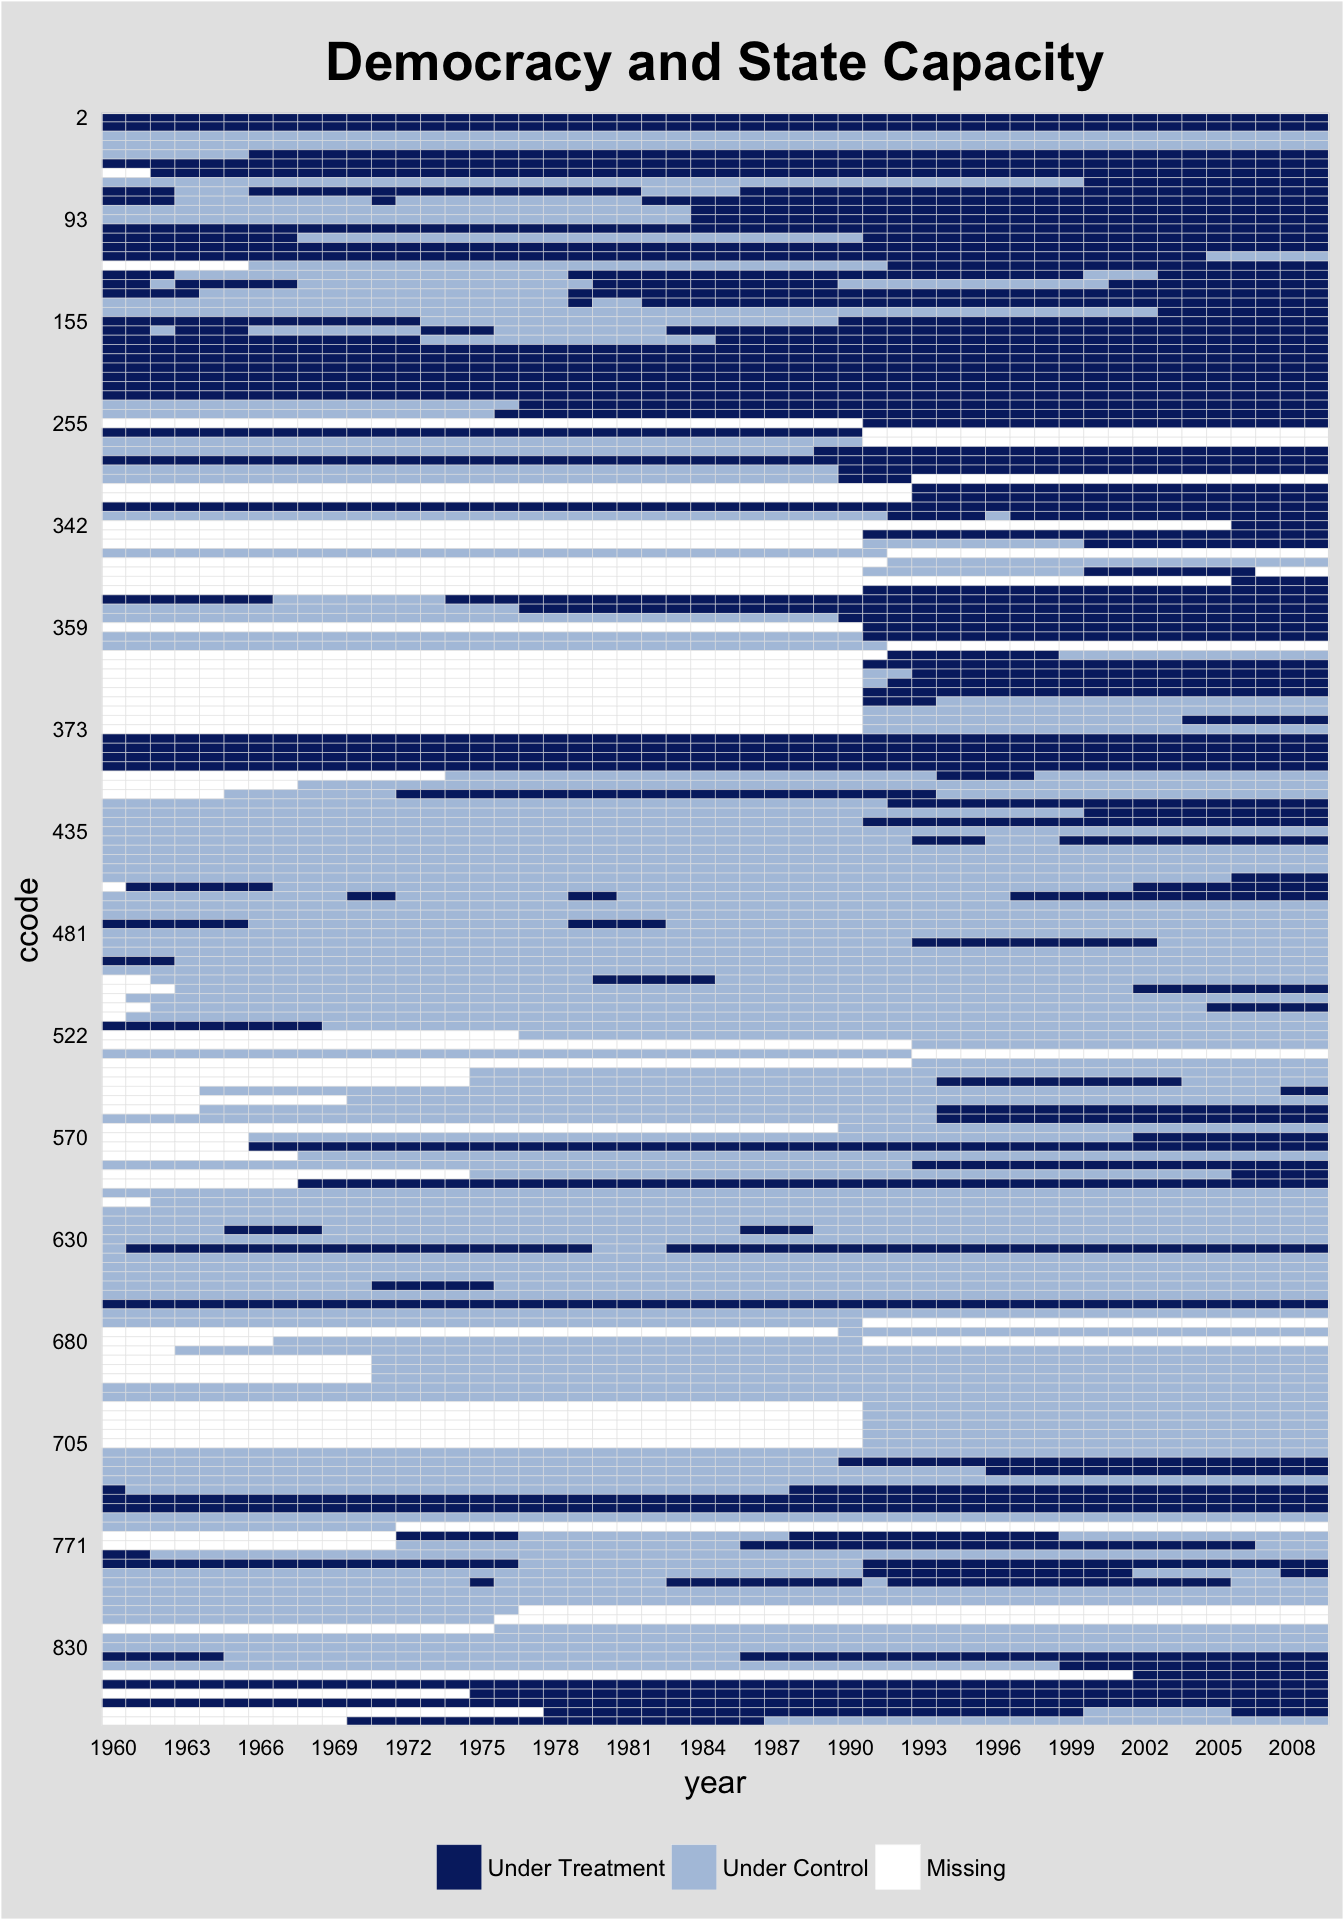
\includegraphics[height=0.8\textheight]{state_capacity.png}}%
  \end{center}
\end{column}
\begin{column}{0.5\textwidth}
\begin{itemize}\itemsep1em 
  \item Recall that our main goal is to predict treated counterfactuals\pause
  \item Taking advantage of the matrix structure, \blue{matrix completion methods} use non-treated data to achieve this goal\pause
  \item The basic idea to find a lower-rank representation of the matrix to impute the \red{``missing data''}\pause 
  \item \textcite{xu2017generalized} is a special case of this approach
\end{itemize}     
\end{column}
\end{columns}
\end{frame}
}
\else {
\begin{frame}[c]
\frametitle{Matrix Completion Methods}
\begin{columns}
\begin{column}{0.5\textwidth}
  \vspace{-1em}
  \begin{center}
  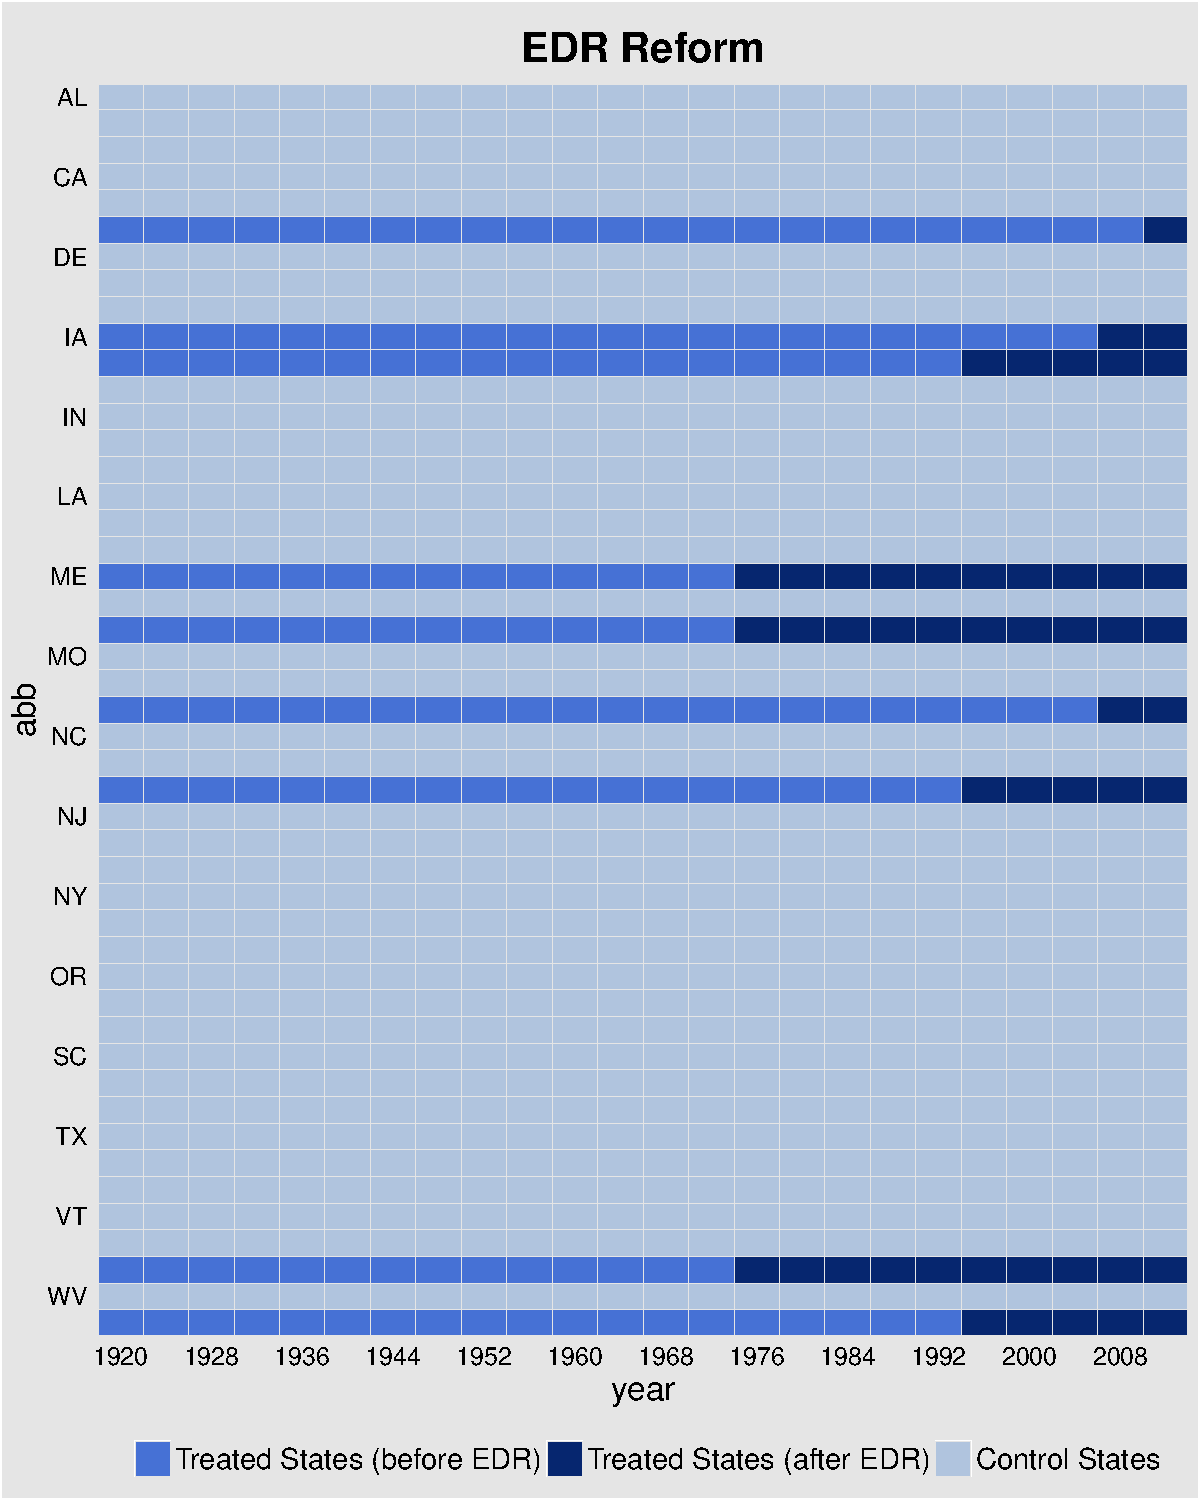
\includegraphics[height=0.8\textheight]{edr_missing0.pdf}
  \end{center}
\end{column}
\begin{column}{0.5\textwidth}
\begin{itemize}\itemsep1em 
  \item Recall that our main goal is to predict treated counterfactuals\pause
  \item Taking advantage of the matrix structure, \underline{matrix completion methods} use non-treated data to achieve this goal\pause
  \item The basic idea to find a lower-rank representation of the matrix to impute the ``missing data''\pause 
  \item \textcite{xu2017generalized} is a special case of this approach
\end{itemize}     
\end{column}
\end{columns}
\end{frame}
}
\fi 

\frame{
\frametitle{Inferential Methods and Diagnostics}
\begin{itemize}\itemsep2em
  \item Non-parametric block bootstrap\medskip
  \begin{itemize}\itemsep0.5em
    \item sample with replacement \underline{across units}\pause
    \item valid when $N$ is large, $\frac{N_{tr}}{N}$ is fixed
  \end{itemize}\pause

  \item A permutation-based test for Sharp Nulls {\small \blue{\parenciteshort{chernozhukov2021exact}}}\medskip
  \begin{itemize}\itemsep0.5em
    \item e.g. $Y_{it}(1) = Y_{it}(0), \forall i\in\T, t>T_{0i}$\pause
    \item randomization \underline{over time} (by blocks) instead of across units\pause
    \item valid if $T$ is large, errors are stationary, weakly dependent, and estimators are consistent or stable
    \item exact if errors are i.i.d.
  \end{itemize}
  \item \textcite{liu2024practical} propose a set of diagnostic tests
\end{itemize}
}


%%%%%%%%%% FM 2015 %%%%%%%%%%%


%%%%%%%%%%%%%%%%%%%%%%%%%%%%%%%%%%%%%%%%%%%%%%%%%%%%%%%%%%%%%
%%%%%%%%%%%%%%%%%%%%%%%%%%%%%%%%%%%%%%%%%%%%%%%%%%%%%%%%%%%%%
%%%%%%%%%%%%%%%%%%%%%%%%%%%%%%%%%%%%%%%%%%%%%%%%%%%%%%%%%%%%%
%%%%%%%%%%%%%%%%%%%%%%%%%%%%%%%%%%%%%%%%%%%%%%%%%%%%%%%%%%%%%

\if\handout0{
\begin{frame}
\frametitle{What We Have Covered So Far}
\addtocounter{framenumber}{-1}
\begin{itemize}\itemsep0.5em
  \item The synthetic control method: a review
  \item The latent factor approach
  \begin{itemize}
    \item The interactive fixed effects model
    \item The matrix completion method
    \item Diagnostics
  \end{itemize}
  \item Next: doubly robust methods --- augmented SCM and synthetic DID
\end{itemize}
\end{frame}
}\fi


\section{Doubly and Triply Robust Methods}

\begin{frame}{Doubly and Triply Robust Methods}
\begin{itemize}\itemsep1em
  \item So far, we've surveyed two groups of methods: (1) those constructing balancing weights; (2) those modeling the conditional outcomes\pause
  \item Combining the two approaches will likely produce doubly robust estimators\pause
  \item Some methods we discussed, including semi-parametric DID and panel matching, are already doing a simple version of it (balancing plus regression)\pause
  \item We review three methods that formally adopt this idea\pause
  \begin{itemize}\itemsep0.5em
    \item Augmented synthetic control {\small\blue{\parenciteshort{benmichael2021augmented}}}: modeling first
    \item Synthetic DID {\small\blue{\parencite{arkhangelsky2021synthetic}}}: weighting first
    \item Triply robust panel estimator {\small\blue{\parenciteall{athey2026triply}}}: unit weights, time weights, and the factor model of the previous section, tuned together
  \end{itemize}
\end{itemize}
\end{frame}


\begin{frame}{Augmented Synthetic Control {\parenciteshort{benmichael2021augmented}}}
\begin{adjustwidth}{-1.5em}{-1.5em}
\begin{itemize}\itemsep1em
  \item Assuming unit $1$ being treated ($D_{1}=1; D_{-1} = 0$), pretreatment covariates $X_{i}$
  \item \textbf{Basic Idea}
  \begin{enumerate}\itemsep0.5em
    \item Run an outcome model (e.g. Ridge, FEct, IFEct, MC, etc.) and obtain model fit $\hat{m}(X_{i})$\pause
    \item Balance on the residual averages, obtaining weights $\hat\gamma_{i}$ for the controls\pause
    \item Treated average is constructed using:
    \begin{align*}
    \hat{Y}^{aug}_{1}(0) = & \underbrace{\sum_{i\in\C}\hat\gamma_{i} Y_{i}}_{SCM}  + 
    \underbrace{\hat{m}(X_{1}) - \sum_{i\in\C}\hat\gamma_{i}\hat{m}(X_{i})}_{debias} \\
    = & \hat{m}(X_{1}) + \sum_{i\in\C}\hat\gamma_{i} \left(Y_{i} - \hat{m}(X_{i})\right)    
    \end{align*}
  \end{enumerate}\vspace{-1em}\pause
  \item The balancing weights take care of the remaining biases from the outcome model; the estimator is thus \red{doubly robust}\pause
  \item Inference via jackknife
\end{itemize}
\end{adjustwidth}
\end{frame}


\frame{
\frametitle{Revisiting California Prop 99}
\vspace{-1em}\begin{center}
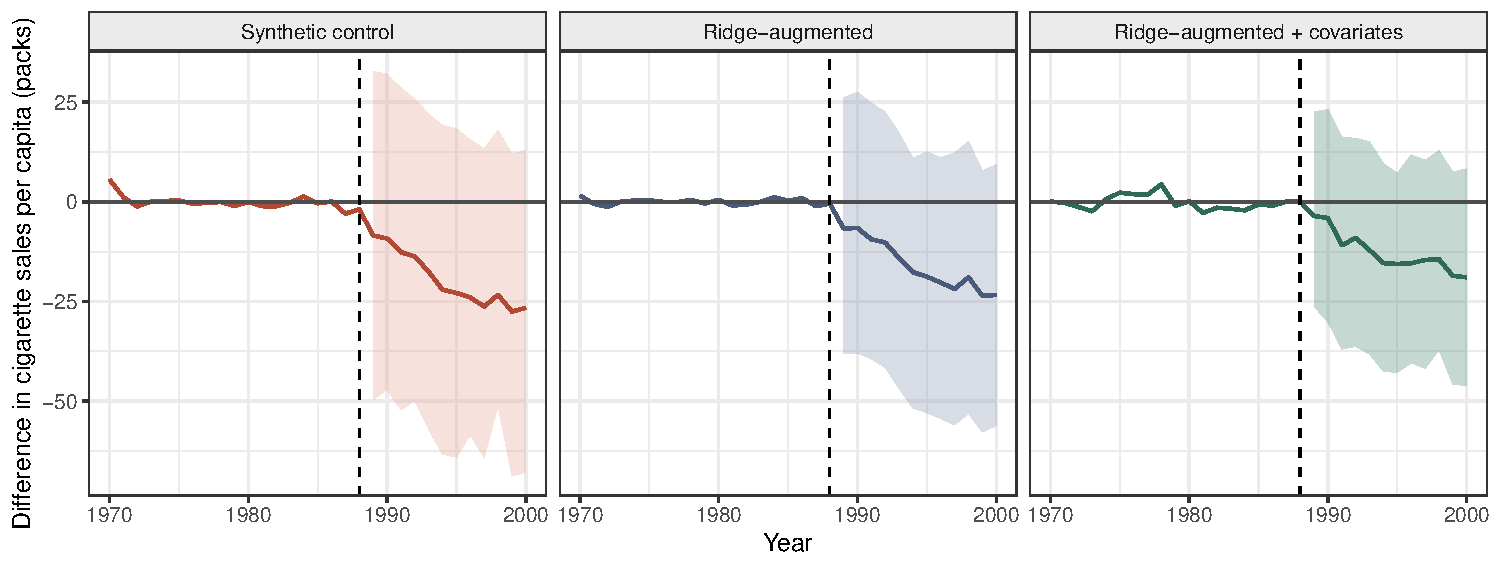
\includegraphics[width = 0.95\textwidth]{augsynth_prop99_2026.pdf}
\end{center}
\slidesource{Own estimates with the \texttt{augsynth} package on the \textcite{abadie2010synthetic} data; bands are jackknife+ intervals (\texttt{augsynth\_prop99\_2026.R}).}
}


\begin{frame}
  \frametitle{Synthetic DID {\parencite{arkhangelsky2021synthetic}}}
  \begin{itemize}
  \item Key insight: weight not only control units, but also pretreatment periods
  \item[] {\footnotesize Notation: the time weights $\lambda_t$ in what follows are unrelated to the factor loadings $\lambda_i$ of the previous section.}
  \end{itemize}\pause
  \begin{figure}[H] 
  \centering 
  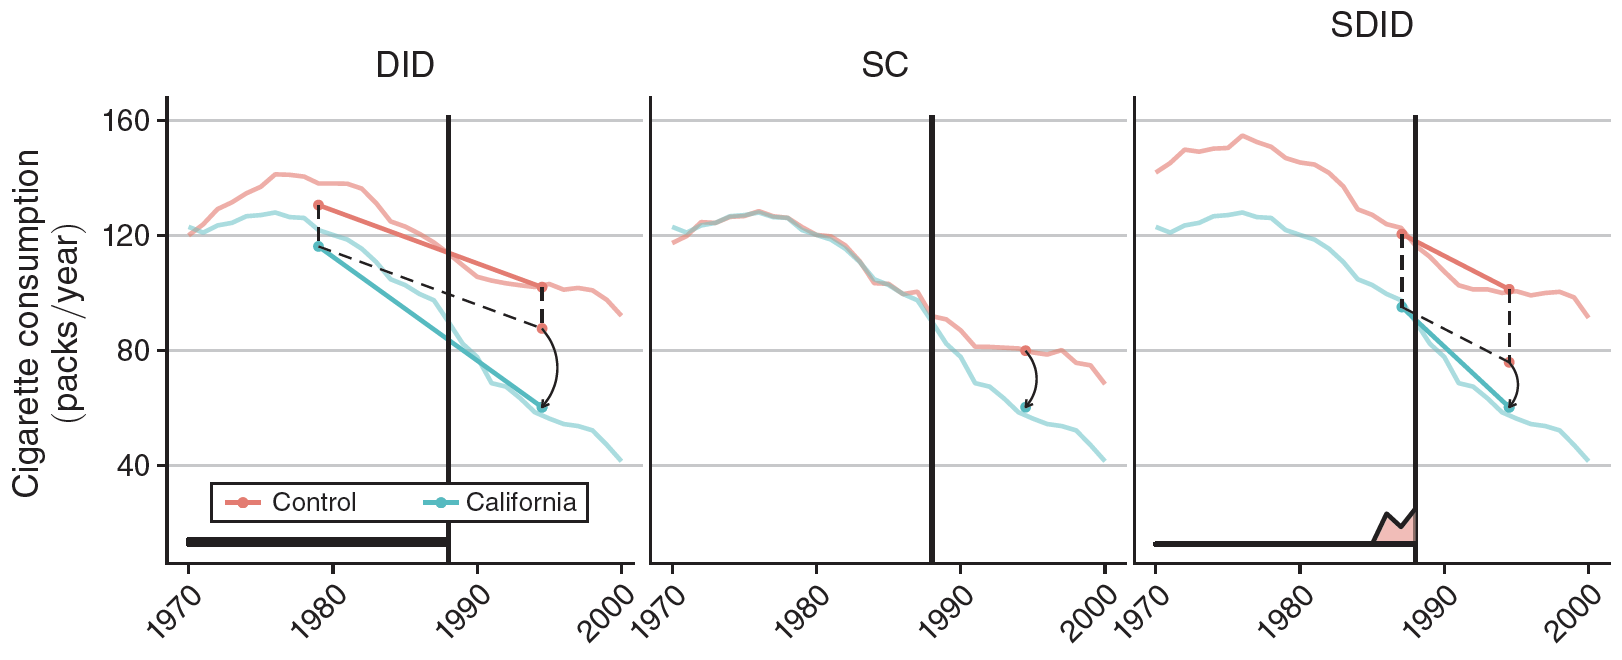
\includegraphics[width=0.9\textwidth]{sdid2.png} 
  \end{figure}
  \slidesource{Figures on the SDID frames are from the authors' slides; see \textcite{arkhangelsky2021synthetic}.}
\end{frame}
  
  
  \begin{frame}
  \frametitle{Unit and Time Weights}
  \begin{itemize}
      \item SC:
      \begin{itemize}
          \item Using \textcolor{blue}{pre-treatment data}, we learn an average of controls that's predictive of California.
          \item Assuming this relationship remains valid post-treatment, we use the \textcolor{red}{same average of controls} to impute treatment-free observations for California
      \end{itemize}\pause
      \item Forecasting:
      \begin{itemize}
          \item Using \textcolor{blue}{controls}, we learn an average of periods forecasting what we see post-treatment
          \item Assuming this relationship remains valid for the treated, we use the \textcolor{red}{same average of periods} to impute treatment-free observations for California
      \end{itemize}\pause
  \end{itemize}
  \begin{figure}[H] 
  \centering 
  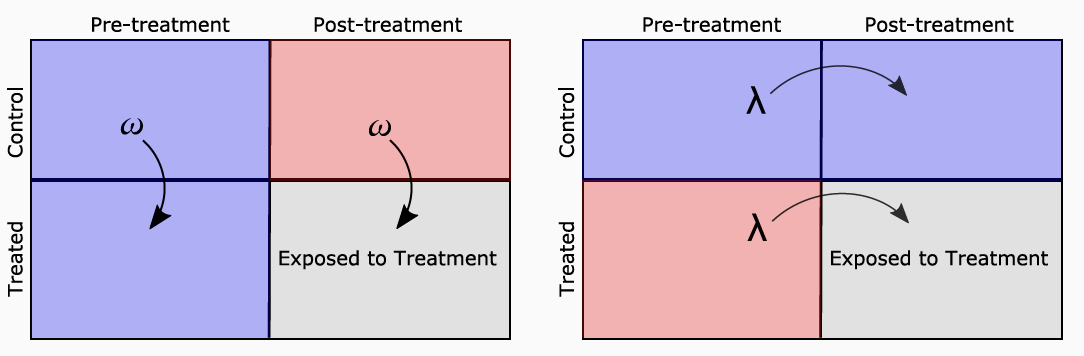
\includegraphics[width=0.7\textwidth]{sdid1.png} 
  \end{figure}
  \slidesource{The authors' slides; see \textcite{arkhangelsky2021synthetic}.}
  \end{frame}
  
  
  \begin{frame}
  \frametitle{Unit and Time Weights}
  \begin{itemize}
      \item Synthetic Diff-in-Diff (SDID)
      \begin{itemize}
          \item Do both synthetic control and forecasting and combine via diff-in-diff
          \item Only one of these relationships has to remain valid (double robustness)
          \item Our synthetic control can be parallel to California
      \end{itemize}
  \end{itemize}
  \begin{figure}[H] 
  \centering 
  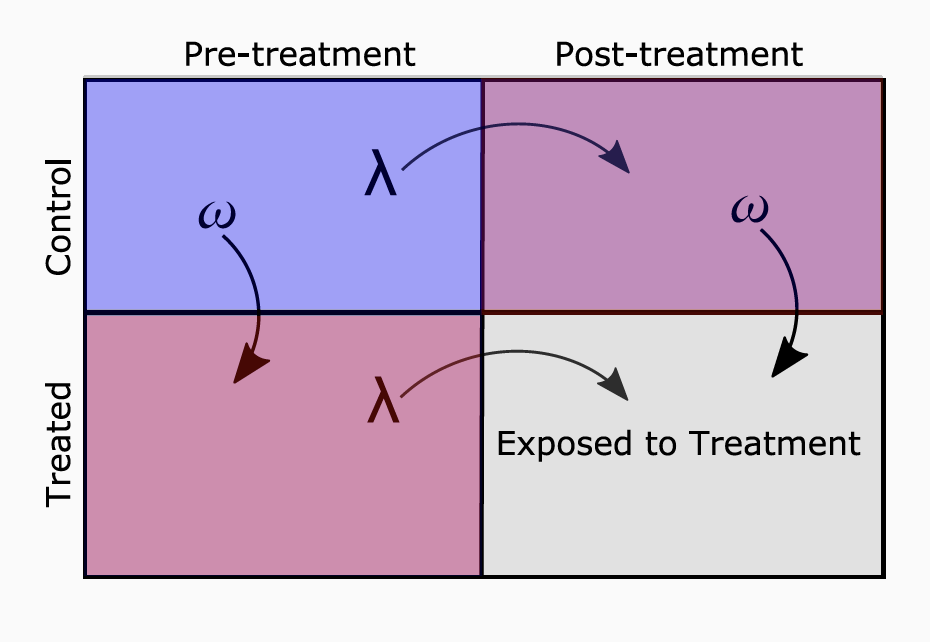
\includegraphics[width=0.55\textwidth]{sdid3.png} 
  \end{figure}
  \slidesource{The authors' slides; see \textcite{arkhangelsky2021synthetic}.}
  \end{frame}
  
  
  \begin{frame}
  \frametitle{SDID}
  \begin{itemize}\itemsep0em\small
  \item[1.] Estimate unit weights $\hat{\omega}$ from pre-treatment data $\Rightarrow$ a synthetic control unit: $
  \hat{\omega}_{0}+\hat{\omega}^{T} Y_{c o, p r e} \approx Y_{\overline{t r}, p r e}.$
  \item[2.] Estimate time weights $\hat{\lambda}$ from control data $\Rightarrow$ a synthetic pre-treatment period: $\hat{\lambda}_{0}+Y_{c o, p r e} \hat{\lambda} \approx Y_{c o, \overline{p o s t}}.$
  \item[3.] Apply diff-in-diff to the resulting synthetic $2 \times 2$ panel by minimizing:
      \[\sum_{i=1}^{N}\sum_{t=1}^{T} (Y_{it} - \mu - \alpha_{i} - \beta_{t} - X_{it}\gamma - D_{it}\tau)^{2}\hat{\omega}_{i}\hat{\lambda}_{t}\]\pause
  \end{itemize}\vspace{-1em}
  \begin{figure}[H] 
  \centering 
  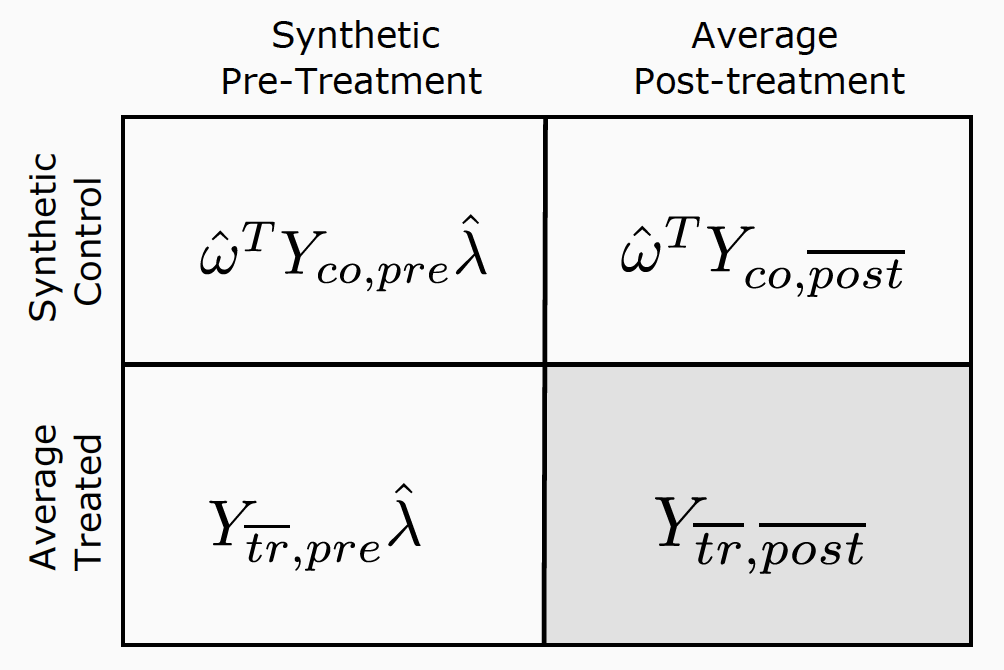
\includegraphics[width=0.32\textwidth]{sdid4.png} 
  \end{figure}\pause
  * Inference via jackknife
  \slidesource{The authors' slides; see \textcite{arkhangelsky2021synthetic}.}
  \end{frame}

\begin{frame}
\frametitle{Triply Robust Panel Estimator {\parenciteall{athey2026triply}}}
\begin{itemize}\itemsep0.7em
  \item SDID weights units and periods around a two-way fixed effects model. TROP adds the third ingredient from the previous section, a \red{low-rank factor component}, and lets the data tune all three\pause
  \item Working model for the untreated outcome: $Y_{it}(0) = \alpha_i + \beta_t + L_{it} + \varepsilon_{it}$, with $L$ low rank\pause
  \item Three components, one tuning parameter each:
  \begin{enumerate}\itemsep0.4em
    \item \textbf{Regression adjustment}: estimate $L$ by nuclear-norm penalized least squares (penalty $\lambda_{nn}$; $\lambda_{nn} = \infty$ switches the factor component off)
    \item \textbf{Unit weights} $\omega_j = \exp(-\lambda_{unit}\, d_{unit}(j, i))$: decay with the mean squared outcome gap between control $j$ and the treated unit over their shared untreated periods
    \item \textbf{Time weights} $\theta_s = \exp(-\lambda_{time}\, |s - t|)$: decay with the distance to the treated period, so the recent past counts most
  \end{enumerate}\pause
  \item Fit the weighted, penalized model on the untreated cells, impute $\hat{Y}_{it}(0) = \hat\alpha_i + \hat\beta_t + \hat{L}_{it}$, and take $\hat\tau_{it} = Y_{it} - \hat{Y}_{it}(0)$; the weights are specific to the treated cell, so any assignment pattern works
\end{itemize}
\end{frame}

\begin{frame}
\frametitle{TROP: Tuning by Leave-One-Out, and Why ``Triply'' Robust}
\begin{itemize}\itemsep0.35em
  \item Choosing $(\lambda_{unit}, \lambda_{time}, \lambda_{nn})$: pretend each untreated cell is treated, impute it from the other untreated cells, and pick the triple whose pseudo-effects are closest to zero,
  \[ Q(\lambda) = \sum_{i,t} (1 - W_{it})\, \hat\tau_{it}(\lambda)^2, \]
  the placebo idea from the synthetic control section, turned into a loss function\pause
  \item The grid nests the menu: flat weights and no factor is DID/TWFE; flat weights with a factor is matrix completion; no factor with particular unit and time weights is synthetic control or SDID\pause
  \item \red{Triple robustness}: with fixed weights the bias is bounded by a \red{product},
  \[ \bigl|\E[\hat\tau - \tau \mid L]\bigr| \;\le\; \underbrace{\|\Delta_u(\omega)\|}_{\text{unit imbalance}} \times \underbrace{\|\Delta_t(\theta)\|}_{\text{time imbalance}} \times \underbrace{\|B\|}_{\text{bias of } \hat{L}} \]
  so it vanishes if the weighted controls match the treated unit's loadings, or the weighted pre-periods match the treated period's factors, or the factor fit is unbiased\pause
  \item ASCM and SDID need one of two things to hold; TROP needs one of three
\end{itemize}
\end{frame}

\begin{frame}
\frametitle{TROP against the Alternatives: RMSE Relative to the Best Estimator}
\begin{center}
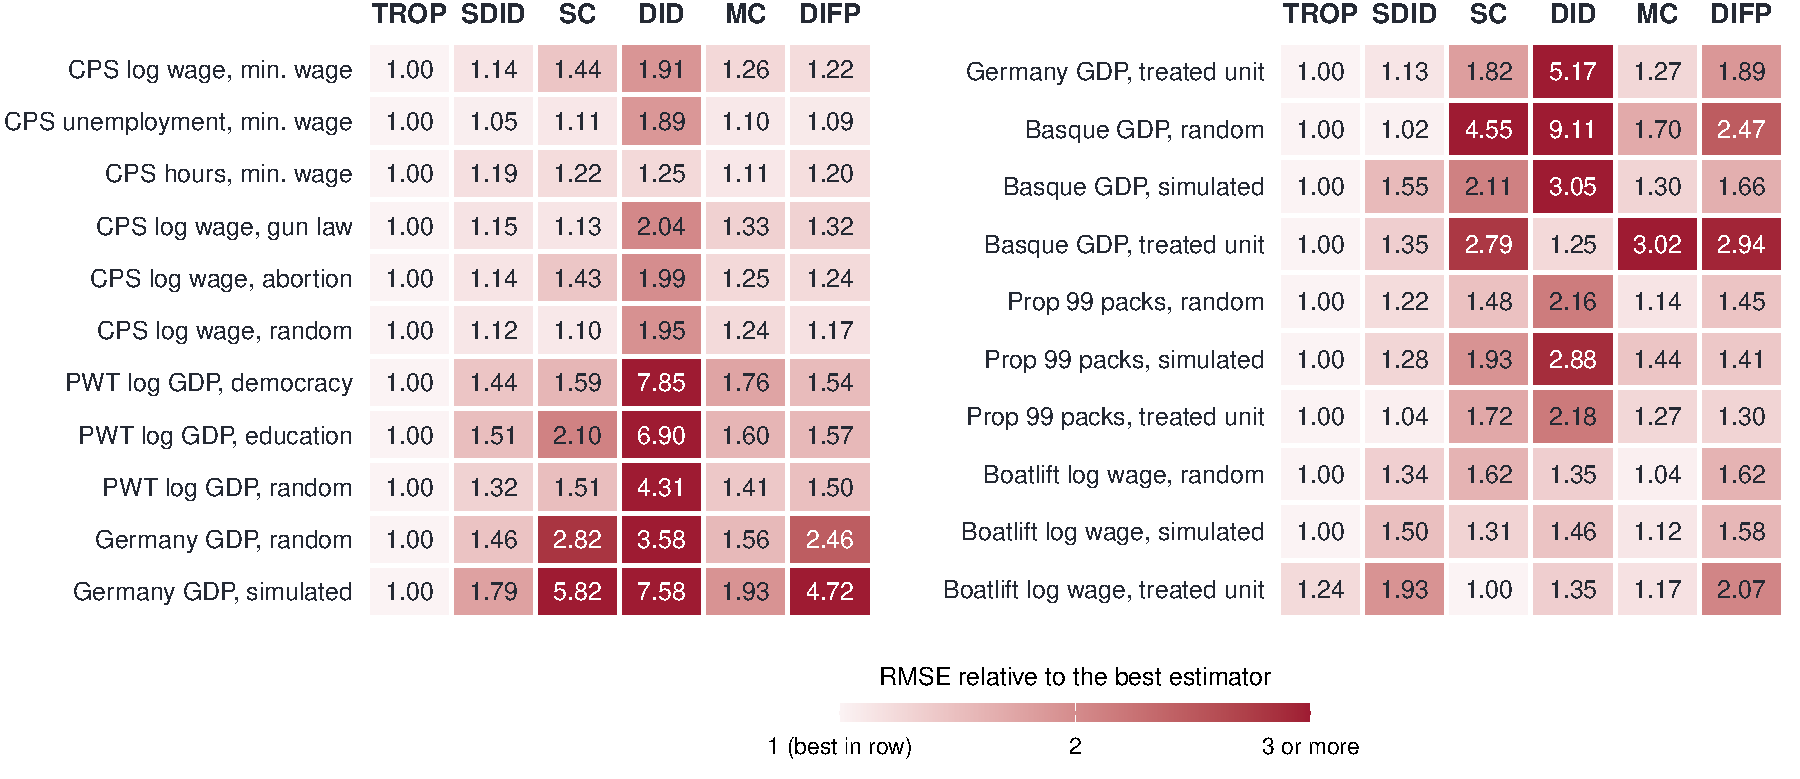
\includegraphics[width=\textwidth, height=0.66\textheight, keepaspectratio]{trop_rmse_2026.pdf}
\end{center}
\vspace{-0.6em}
{\footnotesize Out-of-sample RMSE divided by the smallest RMSE in the row; 21 designs calibrated to real panels, 10 treated units and 10 post periods. DIFP: synthetic control with an intercept. Source: \textciteall{athey2026triply}, Table 1.}
\end{frame}

\begin{frame}
\frametitle{TROP: What the Calibrated Simulations Show}
\begin{itemize}\itemsep0.7em
  \item Semi-synthetic designs: keep a real panel's factor structure and serial correlation, assign treatment as in the application, add a known effect. Panels: CPS wages and unemployment (minimum wage), Penn World Table (democracy), German reunification, the Basque Country, Prop 99, the Mariel boatlift; 21 designs with 10 treated units and 10 post periods\pause
  \item TROP has the lowest RMSE in 20 of the 21. Relative to the best estimator in each design, DID's RMSE reaches 9 times the best (Basque), synthetic control 5.8 times, matrix completion 3 times, SDID 1.9 times\pause
  \item Which ingredient matters: dropping the factor adjustment or the time weights raises RMSE by up to 85--91\%; dropping the unit weights costs at most 10\%; dropping time weights and the factor together can multiply it by five. \red{The recent past matters most}\pause
  \item Their advice: simulate from your own panel and see which estimator wins there; failing that, prefer SDID or TROP to TWFE/DID
\end{itemize}
\end{frame}
  

%%%%%%%%%%%%%%%%%%%%%%%%%%%%%%%%%%%%%%%%%%%%%%%%%%%%%%%%%%%%%
%%%%%%%%%%%%%%%%%%%%%%%%%%%%%%%%%%%%%%%%%%%%%%%%%%%%%%%%%%%%%
%%%%%%%%%%%%%%%%%%%%%%%%%%%%%%%%%%%%%%%%%%%%%%%%%%%%%%%%%%%%%
%%%%%%%%%%%%%%%%%%%%%%%%%%%%%%%%%%%%%%%%%%%%%%%%%%%%%%%%%%%%%

\section{Conclusions}


\begin{frame}
\frametitle{Concluding Remarks}
\begin{itemize}\itemsep0.8em
\item SCM makes the counterfactual construction visible: donor pool, weights, pre-fit, and post-treatment gap.\pause
\item All of these methods learn from the pre-treatment period. The learned relation between treated and donor outcomes must remain useful after treatment.\pause
\item Choose the method after examining the treatment pattern, the number of treated units, and the length of the pre-treatment period.\pause
\item Defend the donor pool, then report placebo and sensitivity checks.
\end{itemize}
\end{frame}


\begin{frame}
\frametitle{Practical Recommendations}

\begin{itemize}\itemsep1em
\item Plot the raw paths and treatment timing before fitting a model.\pause
\item Defend the donor pool using subject knowledge; do not let software choose the comparison set by default.\pause
\item Report pre-fit, gaps, donor weights, and placebo results together.\pause
\item After fixing the research design, use alternative estimators to check sensitivity.
\end{itemize}
\end{frame}

% NOTE (placement, not a disabled slide -- the frame below is live):
% keep this frame ABOVE \appendix. Every frame after \appendix loses the footline, and
% this is a closing slide rather than appendix material. The two References frames are
% still inside the appendix and so still have no footline; move them up here too if
% that is wanted.
\begin{frame}
\frametitle{Where to Read Next}
\begin{itemize}\itemsep0.85em
\item \textcite{abadie2020using}: synthetic controls in comparative case studies.
\item \textcite{benmichael2021augmented}: augmented synthetic control.
\item \textcite{arkhangelsky2021synthetic}: synthetic difference-in-differences.
\item \textciteall{athey2026triply}: the triply robust panel estimator, with simulations calibrated to real panels.
\item \textcite{arkhangelsky2024causal}: DID, fixed effects, factor models, and synthetic controls in a common framework.
\item \textcite{cunningham2021causal}: worked Texas prison example with R code.
\end{itemize}
\end{frame}

\appendix


\setbeamertemplate{frametitle continuation}[from second][(cont.)]
\begin{frame}[t,allowframebreaks=1.0]
  \frametitle{References}
  \referencelist
\end{frame}


\end{document}
